\documentclass[11pt]{article}
\usepackage{debulletin,times,epsfig,subfigure,wrapfig,algorithmic,color,boxedminipage,graphicx,url}

% this is the template for an issue of the Data Engineering Bulletin

% all packages used by any paper must be listed here
%\usepackage{hyperref}
%\usepackage{authblk}
%\setlength{\affilsep}{0em}
%\usepackage{inputenc}
%\usepackage{debulletin}
%\usepackage{times}
%\usepackage{graphicx}
%\usepackage{array}
%\usepackage{wrapfig}
%\usepackage[table]{xcolor}
%\usepackage{tcolorbox}
%\usepackage{amssymb}
%%\usepackage[labelfont=bf,labelsep=space,list=true]{subcaption}
%\usepackage{url}
%\usepackage{mathtools, bm}
%\usepackage{float}
%\usepackage{multirow}
%\usepackage{multicol}
%\usepackage{algorithm}
%\usepackage{subfig}
%\usepackage{algpseudocode}
%\setlength{\intextsep}{10pt plus 2pt minus 2pt}
%\hyphenation{finally}
\usepackage[utf8]{inputenc}

\usepackage{amsmath, amssymb, amsfonts}

\usepackage{hyperref}
\usepackage{enumitem}
\usepackage{xspace} 
%\usepackage{xcolor}
\usepackage{tikz}
\usepackage[T1]{fontenc}
\usepackage{beramono}
\usepackage{listings}
\usepackage{xcolor}

% Prov paper
\usepackage{array}
\usepackage{multirow}
\usepackage{multicol}
\usepackage{hhline}
\usepackage{mathrsfs}  
\usepackage[linesnumbered,ruled]{algorithm2e}
%

% strm privacy
\usepackage[english]{babel}
%

% manos
\usepackage{booktabs} 
\usepackage{epstopdf}
\usepackage{verbatimbox}
\usepackage{multirow} 
%

\usepackage{wrapfig}

\usepackage{graphics}
\usepackage{pifont}
%\usepackage{subcaption} % for subtable
%\usepackage{threeparttable} % for tablenotes




\usepackage[numbers]{natbib}
% \documentclass{article}
% Recommended, but optional, packages for figures and better typesetting:
\usepackage{microtype}
\usepackage{graphicx}
% \usepackage{subfigure}
\usepackage{booktabs} % for professional tables
%\usepackage[table,dvipsnames]{xcolor}
\usepackage{epsfig}
\usepackage{pgfplotstable}
\usepackage{pgfplots}
\usepgfplotslibrary{groupplots}
\usepackage{bbm}
\usepackage{booktabs}
\usepackage{verbatim}
\usepackage[T1]{fontenc}
\usepackage{caption}
\usepackage{siunitx}
\usepackage{xspace}
%\usepackage[colorinlistoftodos,textsize=footnotesize]{todonotes}
%\usepackage[utf8]{inputenc}
\usepackage[autostyle, english=american]{csquotes}
\usepackage{breakurl}




\begin{document}


% please enter real date, vol no, issue no
\bulletindate{March 2022}
\bulletinvolume{45}
\bulletinnumber{1}
\bulletinyear{2022}

% these are files that I have- but your part of the issue can be done without
% them
\IEEElogo{cs.pdf}
\insidefrontcover{incvA19.pdf}
%\insidebackcover[ICDE Conference]{./calls/icde-new-a.ps}

\begin{bulletin}

% the above samples assume the issue is generated from a directory structure of the following sort
% major directory name is month and year of issue
% there are sub-directorys for
% letters: directory name is "letters"
% technical articles: a directory per paper, named for an "author"
% news articles: directory name is "news"
% calls: directory name is "calls

%
%  Editor letters section.  Use the lettersection environment.
%  Each letter is contained in a letter environment, where the two required
%  options to \begin{letter} are the author and the address of the author.
%

\begin{lettersection}

% there will be other letters- and a blank page will appear in your document
% but the special issue part will be fine

\begin{letter}{Letter from the Editor-in-Chief}
{Haixun Wang}{Instacart}
\documentclass[11pt]{article} 

\usepackage{deauthor,times,graphicx}
%\usepackage{url}
\usepackage{hyperref}

\begin{document}
Around the time we published our last issue in March, the nation went
into a lockdown. Life in the last 3 months has been unprecedented in
many ways. As governments around the world scrambled to fight
coronavirus, people in the scientific community, especially those on
the frontline -- doctors, healthcare professionals, medical staff and
researchers -- made heroic efforts and sacrifices to curb the pandemic
and save lives. The data management and data science communities also
sprang to action immediately. Globally, it is the first time that data
driven approaches are being used at such a large scale toward solving
a common problem. Under this backdrop, in this special issue of the
Data Engineering Bulletin edited by Joseph Gonzalez, we feature 8
papers on the topic of {\it digital contact tracing}, a technique that
may prove crucial in the fight against Covid-19.

This issue also features two opinion pieces. Divyakant Agrawal and Amr
El Abbadi's wake-up call on managing data in an untrusted environment
takes us to the fascinating world of cryptocurrencies and
blockchains. It shows what the database community, which was
responsible for creating and perfecting transaction management and
distributed systems, can learn from the blockchain approach when it
comes to handling untrusted behaviours from the underlying
infrastructure. The second opinion piece, written by Jeffrey
D. Ullman, addresses a question on the mind of every data management
person: What is our role in the machine learning and AI revolution?
Have we missed the boat again and become irrelevant? Ullman's
perspective, illustrated by his remake of the well known Conway Venn
Diagram that illustrates the relationship between computer science,
mathematics \& statistics, and domain knowledge is incisive,
thought-provoking, and entertaining at the same time.
\end{document}


\end{letter}
%
\newpage
%
%% your introductory letter goes here
%
%\begin{letter}{Letter from the Special Issue Editor}
\begin{letter}{Letter from the Special Issue Editor} %JF: made it editors, plural
{Sebastian Schelter}{University of Amsterdam \& Ahold Delhaize Research, The Netherlands}
\documentclass[11pt]{article} 

\usepackage{deauthor,times,graphicx}
%\usepackage{url}

\begin{document}

Software applications that learn from data using machine learning (ML) are being deployed in increasing numbers in the real world. Designing and operating such applications introduces novel challenges, which are very different from the challenges encountered in traditional data processing scenarios. ML applications in the real world exhibit a much higher complexity than ``text book'' ML scenarios (e.g., training a classifier on a pre-existing dataset). They do not only have to learn a model, but must define and execute a whole ML pipeline, which includes data preprocessing operations such as data cleaning, standardisation and feature extraction in addition to learning the model, as well as methods for hyperparameter selection and model evaluation. Such ML pipelines are typically deployed in systems for end-to-end machine learning, which require the integration and validation of raw input data from various input sources, as well as infrastructure for deploying and serving the trained models. The system must also manage the lifecycle of data and models in such scenarios, as new (and potentially changing) input data has to be continuously processed, and the corresponding ML models have to be retrained and managed accordingly. The majority of these challenges have only recently begun to attract the attention of the data management community. 
%
A major obstacle is that the behavior of ML-based systems heavily depends on the consumed input data, which can rapidly change, for example due to changed user behavior or due to errors in external sources that produce the inputs. This area represents a gap between the data management and ML communities: research in ML mostly focuses on learning algorithms, and research in data management is mostly concerned with data processing and integration. In this issue, we focus on this gap in data validation for machine learning, and provide perspectives from both the academic and industrial research communities to learn about the state of the art, open problems and to uncover interesting research directions for the future.

The first paper presents \textit{A Data Quality-Driven View of MLOps} and demonstrates how different aspects of data quality propagate through various stages of machine learning development. It connects data quality to the downstream machine learning process, an approach that is also taken by our second paper, which argues that we should move \textit{From Cleaning before ML to Cleaning for ML}. The authors propose an end-to-end approach to take the entire application's semantics and user goals into account when cleaning data, instead of performing the cleaning operations in an isolated manner beforehand.

The next two papers on \textit{Validating Data and Models in Continuous ML pipelines} and \textit{Automated Data Validation in Machine Learning Systems} from Google and Amazon provide us with an industry perspective on the area in the focus of this issue. The first paper describes tools developed at Google for the analysis and validation of two of the most important types of artifacts: Datasets and Models. These tools (which are part of the Tensorflow Extended Platform) are currently deployed in production at Google and other large organizations, and are heavily inspired by well-known principles of data-management systems. The second paper from Amazon reviews some of the solutions developed to validate data at the various stages of a data pipeline in modern ML applications, discusses to what extent these solutions are being used in practice, and outlines research directions for the automation of data validation.

The subsequent paper on \textit{Enhancing the Interactivity of Dataframe Queries by Leveraging Think Time} focuses on the highly exploratory and iterative nature of data validation in the early stages of an ML application, where data scientists start with a limited understanding of the data content and quality, and perform data validation through incremental trial-and-error. The final paper of this issue on \textit{Responsible AI Challenges in End-to-end Machine Learning} completes the view on data validation for machine learning by connecting it with pressing issues from the area of responsible data management.\\ 

Working on this issue has been a privilege for me, and I would like to thank the authors for their  contributions.


\end{document}

\end{letter}

\end{lettersection}

% put the name of your special issue below

\begin{opinionsection}
\begin{opinion}{Data Errors:  Symptoms,  Causes and  Origins}
{Ihab F. Ilyas, Felix  Naumann}{University  of  Waterloo, University of Potsdam}
\documentclass[11pt]{article}
\usepackage{deauthor,graphicx,times}
\usepackage{cite}

% COMMANDS GO HERE
%please list all commands used in your paper, eliminating duplicates

\newtheorem{Example}{\textbf{Example}}


% Your paper submission must be in a folder named with the
% contact author name.

\graphicspath{{author-name/}}

\begin{document}


%\title{Data Errors: Symptoms, Causes and Origins}

%% \author{
%% Ihab F. Ilyas \\
%% University of Waterloo\\ Canada  \\
%%  ilyas@cs.uwaterloo.ca\\
%% \and Felix Naumann\\
%%  Hasso Plattner Institute, University of Potsdam\\Germany \\
%%  felix.naumann@hpi.de
%% }

%% \maketitle

%\begin{abstract}
%\end{abstract}

%%!TEX root = paper.tex
\section{Introduction: Data Errors and their Root Causes}
\label{sec:intro}

With the recent move towards data-centric AI, data quality is now playing an even bigger role in producing sound and reliable insights, predictions and analytics. While the data management community has been working on the problem of data cleaning for decades, the problem remains very much present. Most efforts have focused on error detection~\cite{DBLP:books/acm/IlyasC19}, attempting to leverage symptoms and the manifestations of these errors in data sets to locate and possibly repair them. 
Indeed, the last few years witnessed significant advances in automating error detection and repairing~\cite{holoclean,holodetect,raha,yeye-unidetect} by probabilistically modelling dirty data sets, and reasoning about error detection and repair as structured prediction problems~\cite{puds,uai_heidari}. In this opinion piece, we present our views on how to further advance the field of data cleaning, and go beyond treating the symptoms of the problem and understand what it takes to treat the causes and the sources of these anomalies and errors.

Tracking errors to their sources is not a new quest of the research community~\cite{DBLP:conf/sigmod/ChalamallaIOP14, DBLP:conf/sigmod/WangM017, DBLP:journals/ftdb/GlavicMR21}. So why are we revisiting it now? %The main observation that motivates this discussion is 
The way current research currently reasons about the root causes of data errors is still, in our opinion, limited. \emph{Tracking errors to sources} has often been framed as  ``computational'' provenance that represents \emph{what} was involved in computing a final data product and possibly \emph{how} this product was computed. The main goal of these provenance-based error tracking systems is projecting errors detected in downstream applications all the way to upstream data sources, where they should be fixed~\cite{DBLP:conf/sigmod/ChalamallaIOP14}.  While the principle is sound, multiple issues often complicate this approach. First, as data processing pipelines become more complex, with cascades of complex machine learning models, capturing this rich provenance information becomes harder, as most if not all of the input is involved in producing the output. Recent progress, however, has been made in tracking responsibility of training data, for example, in the predictions of complex models~\cite{DBLP:journals/corr/abs-2002-08484,pmlr-koh-Liang,DBLP:journals/corr/abs-2202-00622}. Second, even with advances in modelling the responsibility of input sources in the observations in output analytics reports, fixing the sources does not mean that errors have been fixed at their true ``roots'' -- their point of creation; these raw data sources are often the results of other processes not modelled at all in the computational data pipelines, such as grading tasks of humans, sensor readings, and extraction scripts from logs and documents.  

Hence, we argue that effective management of data errors and the next-generation data cleaning systems require a more profound understanding of the root causes data errors. These systems should: (1)~distinguish between \emph{why} errors occur and the processes that generated them in the first place, and \emph{how}  these errors manifest themselves as bad data symptoms (e.g., violations of integrity constraints and appearing as outlying values), and (2)~explicitly model these data generation processes to allow for new process repair actions that go beyond fixing raw data sources. 

% NEED TO INTEGRATE THE FOLLOWING SOMEHOW 
%
%In the absence of any context, a data element\footnote{For now, we formulate our definitions in the most general way by referring to ``data elements'', which can manifest as individual values, rows, columns, objects, graphs, tables or entire datasets. Later, we supply details on this ``what'' question.} cannot constitute an error -- it just ``is''. However, data elements do not exist outside some context: they were somehow produced and shall somehow be consumed. Only this context allows us to identify a data element as erroneous. We can ask \emph{how} the element is an error: how do we notice it as erroneous, what symptoms does it hold? These symptoms exist only in the context of the consumption of the data element. For instance, data might violate some external constraint or assumption. It might be an outlier, compared to other data elements. A relation might be missing some tuples or have some duplicated tuples.

%Given such identified errors, we can ask the obvious next question: \emph{Why} do we observe the error, how did it appear in the data? Possible answers to these questions are the provenance of the data, and the mode in which the data was originally created. For instance, human data entry can create such errors, or faulty sensors produce erroneous data.



%!TEX root = paper.tex
\section{Introduction: Data Errors and their Root Causes}
\label{sec:intro}

With the recent move towards data-centric AI, data quality is now playing an even bigger role in producing sound and reliable insights, predictions and analytics. While the data management community has been working on the problem of data cleaning for decades, the problem remains very much present. Most efforts have focused on error detection~\cite{DBLP:books/acm/IlyasC19}, attempting to leverage symptoms and the manifestations of these errors in data sets to locate and possibly repair them. 
Indeed, the last few years witnessed significant advances in automating error detection and repairing~\cite{holoclean,holodetect,raha,yeye-unidetect} by probabilistically modelling dirty data sets, and reasoning about error detection and repair as structured prediction problems~\cite{puds,uai_heidari}. In this opinion piece, we present our views on how to further advance the field of data cleaning, and go beyond treating the symptoms of the problem and understand what it takes to treat the causes and the sources of these anomalies and errors.

Tracking errors to their sources is not a new quest of the research community~\cite{DBLP:conf/sigmod/ChalamallaIOP14, DBLP:conf/sigmod/WangM017, DBLP:journals/ftdb/GlavicMR21}. So why are we revisiting it now? %The main observation that motivates this discussion is 
The way current research currently reasons about the root causes of data errors is still, in our opinion, limited. \emph{Tracking errors to sources} has often been framed as  ``computational'' provenance that represents \emph{what} was involved in computing a final data product and possibly \emph{how} this product was computed. The main goal of these provenance-based error tracking systems is projecting errors detected in downstream applications all the way to upstream data sources, where they should be fixed~\cite{DBLP:conf/sigmod/ChalamallaIOP14}.  While the principle is sound, multiple issues often complicate this approach. First, as data processing pipelines become more complex, with cascades of complex machine learning models, capturing this rich provenance information becomes harder, as most if not all of the input is involved in producing the output. Recent progress, however, has been made in tracking responsibility of training data, for example, in the predictions of complex models~\cite{DBLP:journals/corr/abs-2002-08484,pmlr-koh-Liang,DBLP:journals/corr/abs-2202-00622}. Second, even with advances in modelling the responsibility of input sources in the observations in output analytics reports, fixing the sources does not mean that errors have been fixed at their true ``roots'' -- their point of creation; these raw data sources are often the results of other processes not modelled at all in the computational data pipelines, such as grading tasks of humans, sensor readings, and extraction scripts from logs and documents.  

Hence, we argue that effective management of data errors and the next-generation data cleaning systems require a more profound understanding of the root causes data errors. These systems should: (1)~distinguish between \emph{why} errors occur and the processes that generated them in the first place, and \emph{how}  these errors manifest themselves as bad data symptoms (e.g., violations of integrity constraints and appearing as outlying values), and (2)~explicitly model these data generation processes to allow for new process repair actions that go beyond fixing raw data sources. 

% NEED TO INTEGRATE THE FOLLOWING SOMEHOW 
%
%In the absence of any context, a data element\footnote{For now, we formulate our definitions in the most general way by referring to ``data elements'', which can manifest as individual values, rows, columns, objects, graphs, tables or entire datasets. Later, we supply details on this ``what'' question.} cannot constitute an error -- it just ``is''. However, data elements do not exist outside some context: they were somehow produced and shall somehow be consumed. Only this context allows us to identify a data element as erroneous. We can ask \emph{how} the element is an error: how do we notice it as erroneous, what symptoms does it hold? These symptoms exist only in the context of the consumption of the data element. For instance, data might violate some external constraint or assumption. It might be an outlier, compared to other data elements. A relation might be missing some tuples or have some duplicated tuples.

%Given such identified errors, we can ask the obvious next question: \emph{Why} do we observe the error, how did it appear in the data? Possible answers to these questions are the provenance of the data, and the mode in which the data was originally created. For instance, human data entry can create such errors, or faulty sensors produce erroneous data.


%%!TEX root = paper.tex
\section{Reasoning about the How: The Symptoms of Errors}
\label{sec:how}

In its most general form, information quality is defined as ``fitness for use''~\cite{Strong96}, i.e., its definition focuses on the use case, the application, the \emph{context} of the data at hand. Most, if not all, error detection methods make heavy use of this context. They search for and focus on the \emph{symptoms} of poor data quality and ask the question \emph{how} a particular data element is an error.
We exemplify this insight with selected examples of traditional error detection problems and their solutions.
\begin{description}
  \item[Outliers] Already by definition, outliers can be recognized only in the context of other data elements -- only these ``inliers'' make some other value an outlier. Typical outlier detection methods create a model to represent normal/typical values and mark as outliers all those values that do not fit the model~\cite{Aggarwal2013}. Whether an outlier is, in fact, an error is application-dependent and user-defined.
  
  \emph{How} is an outlier a data error? It is very different from all \emph{other} data elements, suggesting it is not the intended value for this data item.
  
  \item[Constraint violations] Constraints, such as key-constraints, dependencies, or denial constraints can be used to express the validity of a data instance. These rules are specified by experts or discovered with data profiling methods~\cite{Abedjan2018}. Rarely do they refer to individual data elements; rather they forbid the existence of some elements in the presence of others, such as a key-constraint denying any other record with the same key value. Discovering and cleaning such violations is an active research area~\cite{IlyasC15}.
  
  \emph{How} does a data element violate a constraint? It exists in the presence of some \emph{other} data element. While this is not an error on its own, the collection of these values cannot be part of the intended correct data instance. %, together with which it violates the constraint.
  
  \item[Duplicates] Within a dataset, duplicate records are multiple different representations of the same real-world entity~\cite{Naumann10}. To clean a dataset, such erroneous duplicates must be detected and then merged or eliminated. Identifying a duplicated record is, by definition, possible only by regarding other records, i.e., only in the context of the entire relation. Typical approaches intelligently create duplicate candidate pairs and then determine their similarity to decide whether they are indeed duplicates~\cite{Papadakis21}.
  
  \emph{How} is a duplicate an error? It represents the same real-world object as some \emph{other} data element, with possibly other types of errors causing a different representation.
  
  \item[Missing values] Missing values are easy to detect when they appear as null values in databases or empty strings in files. In more complex cases, ``disguised missing values'' can be recognized only by regarding their context, which usually comprises the other values in the column~\cite{FAHES_18}. 
  The typical means to ``clean'' missing values is to impute their value, again based on their context, usually the non-missing values in a column.
  
  \emph{How} is a missing value an error? It is explicitly represented to indicate an error. However, the difficulty in the case of missing value relates to the interpretation of ``null'' as {\em we don't know the value, but we should} as opposed to schema issues, for example, a relational employees table with some employees who do not have middle names.
\end{description}

Data cleaning, as a means to alleviate the symptoms of poor data quality, is an established and important research and development field, relying heavily on the context of data and its use in applications. Next, we move backwards along the data processing pipeline to explore not these symptoms, but their causes.
%!TEX root = paper.tex
\section{Reasoning about the How: The Symptoms of Errors}
\label{sec:how}

In its most general form, information quality is defined as ``fitness for use''~\cite{Strong96}, i.e., its definition focuses on the use case, the application, the \emph{context} of the data at hand. Most, if not all, error detection methods make heavy use of this context. They search for and focus on the \emph{symptoms} of poor data quality and ask the question \emph{how} a particular data element is an error.
We exemplify this insight with selected examples of traditional error detection problems and their solutions.
\begin{description}
  \item[Outliers] Already by definition, outliers can be recognized only in the context of other data elements -- only these ``inliers'' make some other value an outlier. Typical outlier detection methods create a model to represent normal/typical values and mark as outliers all those values that do not fit the model~\cite{Aggarwal2013}. Whether an outlier is, in fact, an error is application-dependent and user-defined.
  
  \emph{How} is an outlier a data error? It is very different from all \emph{other} data elements, suggesting it is not the intended value for this data item.
  
  \item[Constraint violations] Constraints, such as key-constraints, dependencies, or denial constraints can be used to express the validity of a data instance. These rules are specified by experts or discovered with data profiling methods~\cite{Abedjan2018}. Rarely do they refer to individual data elements; rather they forbid the existence of some elements in the presence of others, such as a key-constraint denying any other record with the same key value. Discovering and cleaning such violations is an active research area~\cite{IlyasC15}.
  
  \emph{How} does a data element violate a constraint? It exists in the presence of some \emph{other} data element. While this is not an error on its own, the collection of these values cannot be part of the intended correct data instance. %, together with which it violates the constraint.
  
  \item[Duplicates] Within a dataset, duplicate records are multiple different representations of the same real-world entity~\cite{Naumann10}. To clean a dataset, such erroneous duplicates must be detected and then merged or eliminated. Identifying a duplicated record is, by definition, possible only by regarding other records, i.e., only in the context of the entire relation. Typical approaches intelligently create duplicate candidate pairs and then determine their similarity to decide whether they are indeed duplicates~\cite{Papadakis21}.
  
  \emph{How} is a duplicate an error? It represents the same real-world object as some \emph{other} data element, with possibly other types of errors causing a different representation.
  
  \item[Missing values] Missing values are easy to detect when they appear as null values in databases or empty strings in files. In more complex cases, ``disguised missing values'' can be recognized only by regarding their context, which usually comprises the other values in the column~\cite{FAHES_18}. 
  The typical means to ``clean'' missing values is to impute their value, again based on their context, usually the non-missing values in a column.
  
  \emph{How} is a missing value an error? It is explicitly represented to indicate an error. However, the difficulty in the case of missing value relates to the interpretation of ``null'' as {\em we don't know the value, but we should} as opposed to schema issues, for example, a relational employees table with some employees who do not have middle names.
\end{description}

Data cleaning, as a means to alleviate the symptoms of poor data quality, is an established and important research and development field, relying heavily on the context of data and its use in applications. Next, we move backwards along the data processing pipeline to explore not these symptoms, but their causes.

%%!TEX root = paper.tex
\section{Reasoning about the Why: The Causes of Errors}
\label{sec:why}

It is time to ask (and answer) the \emph{why} question!
Existing work in the area of data quality, error detection and data cleaning almost exclusively focuses on alleviating the symptoms, rather than removing the cause of the error.
None of the methods asks \emph{why} a particular value is missing, why duplicates exist in the data, why violations occur. Answers as to ``why'' include: faulty (human) data entry, such as missing entries, misplaced values, typos, and vandalism; faulty reading from sensors; missed or not-propagated updates; faulty computations; and misconfigured data pipelines. 

While researchers and practitioners (and medical doctors) will acknowledge the truism that problems are best addressed at their source rather than treating their symptoms, the research community has not adequately addressed this opportunity possibly for several reasons:
\begin{itemize}
    \item In some scenarios, once errors are detected, it is too late -- fixing their cause is futile because the data was intended for a one-time use.
    \item Often, the creation of data is out of the control of the data engineers or data consumers: the data stems from an external source and the data creation can be influenced only through human intervention, such as communicating with the data owners or creators.
    \item Modifying or improving the data creation process is difficult or impossible, for instance due to technical or human limitations: sensors have an inherent error margin; humans are not infallible, etc.
    \item Data processing pipelines have become so complex, that treating the symptoms is the easier short-term goal with quick rewards.
\end{itemize}

Knowledge of the cause of an error and not only its symptom can improve cleaning methods and can help avoid such errors in the first place. To seize this opportunity, multiple challenges must be overcome:
\begin{itemize}
    \item \emph{Modelling} the processes and data generators (including humans) in the system, instead of modelling only the data and errors.

    \item \emph{Detection} of data errors without context and detection of erroneous data processes.
    
    \item Extending the notion of \emph{provenance} to include (possibly faulty) processes, computation (internal provenance), and data generation steps (external provenance). More on this in Section\ref{sec:provenance}.
    
    \item Designing of algorithms and systems to efficiently and effectively trace such extended provenance.
    
    \item Designing \emph{repair} operations for such errors and processes, which need to reach beyond the mere deletion or replacement of data instances that is the currently common approach.

%    \item Algorithms that can point to these new things
\end{itemize}

These challenges can be summarized as creating a more holistic view of data creation and consumption than is currently practiced. Especially the extended notion of provenance deserves a closer look in the next section.

%existing work: Modelling the process or Cleaning actions at the source

%Definition of cause of error: SOME TEXT. Understanding the cause of an error asks ``Why do we observe this error?''

%Raw-data generative process (link to ICDT paper by Ihab, and others)


%``So I'll remove the cause. But not. The symptom!'' Dr.\ Frank N.\ Furter, Rocky Horror Picture Show
%!TEX root = paper.tex
\section{Reasoning about the Why: The Causes of Errors}
\label{sec:why}

It is time to ask (and answer) the \emph{why} question!
Existing work in the area of data quality, error detection and data cleaning almost exclusively focuses on alleviating the symptoms, rather than removing the cause of the error.
None of the methods asks \emph{why} a particular value is missing, why duplicates exist in the data, why violations occur. Answers as to ``why'' include: faulty (human) data entry, such as missing entries, misplaced values, typos, and vandalism; faulty reading from sensors; missed or not-propagated updates; faulty computations; and misconfigured data pipelines. 

While researchers and practitioners (and medical doctors) will acknowledge the truism that problems are best addressed at their source rather than treating their symptoms, the research community has not adequately addressed this opportunity possibly for several reasons:
\begin{itemize}
    \item In some scenarios, once errors are detected, it is too late -- fixing their cause is futile because the data was intended for a one-time use.
    \item Often, the creation of data is out of the control of the data engineers or data consumers: the data stems from an external source and the data creation can be influenced only through human intervention, such as communicating with the data owners or creators.
    \item Modifying or improving the data creation process is difficult or impossible, for instance due to technical or human limitations: sensors have an inherent error margin; humans are not infallible, etc.
    \item Data processing pipelines have become so complex, that treating the symptoms is the easier short-term goal with quick rewards.
\end{itemize}

Knowledge of the cause of an error and not only its symptom can improve cleaning methods and can help avoid such errors in the first place. To seize this opportunity, multiple challenges must be overcome:
\begin{itemize}
    \item \emph{Modelling} the processes and data generators (including humans) in the system, instead of modelling only the data and errors.

    \item \emph{Detection} of data errors without context and detection of erroneous data processes.
    
    \item Extending the notion of \emph{provenance} to include (possibly faulty) processes, computation (internal provenance), and data generation steps (external provenance). More on this in Section\ref{sec:provenance}.
    
    \item Designing of algorithms and systems to efficiently and effectively trace such extended provenance.
    
    \item Designing \emph{repair} operations for such errors and processes, which need to reach beyond the mere deletion or replacement of data instances that is the currently common approach.

%    \item Algorithms that can point to these new things
\end{itemize}

These challenges can be summarized as creating a more holistic view of data creation and consumption than is currently practiced. Especially the extended notion of provenance deserves a closer look in the next section.

%existing work: Modelling the process or Cleaning actions at the source

%Definition of cause of error: SOME TEXT. Understanding the cause of an error asks ``Why do we observe this error?''

%Raw-data generative process (link to ICDT paper by Ihab, and others)


%``So I'll remove the cause. But not. The symptom!'' Dr.\ Frank N.\ Furter, Rocky Horror Picture Show
%%!TEX root = paper.tex
\section{True Data Provenance}
\label{sec:provenance}

Provenance is powerful tool for {\em tracking} data artifacts. In the context of this paper, one might think of it as a way to identify the \emph{where} of the data error's story. Most practical and effective cleaning solutions follow a clean-and-evaluate lifecycle~\cite{Ilyas16DE}, which leverages the computational provenance of data analytics to track data errors to their sources, and attempts to provide explanations that lead to cleaning actions. This typical lifecycle is depicted in Figure~\ref{fig:lifecycle}. 
\begin{figure*}[ht]
  \centering
  \includegraphics[width=0.6\textwidth]{lifecycle}
  \caption{Clean-and-Evaluate Loop~\cite{Ilyas16DE}}
  \label{fig:lifecycle}
\end{figure*}

Provenance and lineage systems focus on describing how the analytical {\em report views} are computed from the sources. For example, Scorpion~\cite{DBLP:journals/pvldb/0002M13}, DBRx~\cite{DBLP:conf/sigmod/ChalamallaIOP14} and QFix~\cite{DBLP:conf/sigmod/WangM017} (and many other followup work) are  solutions that trace back the tuples that contributed to the problems in the target to explain and help fix these errors at data sources. A recent survey summarizes the large body of work in debugging data-driven systems and explain what users see downstream from processing raw data~\cite{DBLP:journals/ftdb/GlavicMR21}. As these processing pipelines become more complex with cascades of large machine learning models, tracing errors in final predictions back to their causes can be very challenging. However, there is recent progress that can help us reason about observations in model predictions and track them back to errors in training data~\cite{DBLP:journals/corr/abs-2202-00622}.

The question becomes: \emph{is explaining errors in final analytics or predictions in terms of data sources enough?} What we refer to as ``raw data sources''  are often cut off the processes that generated these data, such as the human grader that input that data, the extraction script that generated this data from a webpage, or a presentation of the complex data pipeline that ran in a different software stack and generated this source data. From our discussions and involvement with large enterprises over the last decade, we argue that this decoupling is often due to two main reasons:
\begin{itemize}
\item \emph{Difficulty of integrating data processes in provenance systems:} Representing the process that generated the data might require expressive (and hence  complex) provenance systems. For example semiring-based  provenance systems have been extended  to capture information about external inputs (e.g., user choices), and  to capture process executions~\cite{DBLP:journals/vldb/DeutchMT15}; and in the context of scientific workflows,  the need for a control-flow driven workflow provenance model in contrast to the traditional  data-driven execution provenance paradigm has been explored~\cite{DBLP:journals/dke/ButtF21}.

\item \emph{Loss of provenance continuity across systems:}  We might be very careful in collecting and adequately presenting provenance information in the data pipelines we control. However, as the final data product (e.g., predictions, views, aggregates, or transformed data sets) get pushed to the downstream tasks, they are often treated as ``source data'' and downstream pipelines fail to  consume the associated provenance information.
\end{itemize}

Understandably, these are hard problems to tackle and part of the challenge is not even technical and it involves standardizing data provenance representation across business units and different software stacks. However, this might suggest new research directions; for example, we might prefer developing simpler and less expressive provenance models that target interoperability and ease of propagation over representation power of the underlying computations. Another example is that propagating standard meta-data that ties data sources to central data governance and catalogs can be part of the integrity constraints and sanity checks. We suggest also extending meta-data representation of data sources to include {\em repair actions} that reference a controlled vocabulary or a {\em repairing ontology} tapping into the large body of work in work flow and business processes management.





%!TEX root = paper.tex
\section{True Data Provenance}
\label{sec:provenance}

Provenance is powerful tool for {\em tracking} data artifacts. In the context of this paper, one might think of it as a way to identify the \emph{where} of the data error's story. Most practical and effective cleaning solutions follow a clean-and-evaluate lifecycle~\cite{Ilyas16DE}, which leverages the computational provenance of data analytics to track data errors to their sources, and attempts to provide explanations that lead to cleaning actions. This typical lifecycle is depicted in Figure~\ref{fig:lifecycle}. 
\begin{figure*}[ht]
  \centering
  \includegraphics[width=0.6\textwidth]{letters/lifecycle}
  \caption{Clean-and-Evaluate Loop~\cite{Ilyas16DE}}
  \label{fig:lifecycle}
\end{figure*}

Provenance and lineage systems focus on describing how the analytical {\em report views} are computed from the sources. For example, Scorpion~\cite{DBLP:journals/pvldb/0002M13}, DBRx~\cite{DBLP:conf/sigmod/ChalamallaIOP14} and QFix~\cite{DBLP:conf/sigmod/WangM017} (and many other followup work) are  solutions that trace back the tuples that contributed to the problems in the target to explain and help fix these errors at data sources. A recent survey summarizes the large body of work in debugging data-driven systems and explain what users see downstream from processing raw data~\cite{DBLP:journals/ftdb/GlavicMR21}. As these processing pipelines become more complex with cascades of large machine learning models, tracing errors in final predictions back to their causes can be very challenging. However, there is recent progress that can help us reason about observations in model predictions and track them back to errors in training data~\cite{DBLP:journals/corr/abs-2202-00622}.

The question becomes: \emph{is explaining errors in final analytics or predictions in terms of data sources enough?} What we refer to as ``raw data sources''  are often cut off the processes that generated these data, such as the human grader that input that data, the extraction script that generated this data from a webpage, or a presentation of the complex data pipeline that ran in a different software stack and generated this source data. From our discussions and involvement with large enterprises over the last decade, we argue that this decoupling is often due to two main reasons:
\begin{itemize}
\item \emph{Difficulty of integrating data processes in provenance systems:} Representing the process that generated the data might require expressive (and hence  complex) provenance systems. For example semiring-based  provenance systems have been extended  to capture information about external inputs (e.g., user choices), and  to capture process executions~\cite{DBLP:journals/vldb/DeutchMT15}; and in the context of scientific workflows,  the need for a control-flow driven workflow provenance model in contrast to the traditional  data-driven execution provenance paradigm has been explored~\cite{DBLP:journals/dke/ButtF21}.

\item \emph{Loss of provenance continuity across systems:}  We might be very careful in collecting and adequately presenting provenance information in the data pipelines we control. However, as the final data product (e.g., predictions, views, aggregates, or transformed data sets) get pushed to the downstream tasks, they are often treated as ``source data'' and downstream pipelines fail to  consume the associated provenance information.
\end{itemize}

Understandably, these are hard problems to tackle and part of the challenge is not even technical and it involves standardizing data provenance representation across business units and different software stacks. However, this might suggest new research directions; for example, we might prefer developing simpler and less expressive provenance models that target interoperability and ease of propagation over representation power of the underlying computations. Another example is that propagating standard meta-data that ties data sources to central data governance and catalogs can be part of the integrity constraints and sanity checks. We suggest also extending meta-data representation of data sources to include {\em repair actions} that reference a controlled vocabulary or a {\em repairing ontology} tapping into the large body of work in work flow and business processes management.






%\input{5_otherquestions}
%\section{Conclusion}
\label{sec:conc}

To conclude, we suggest opening a new chapter of data quality and data cleaning that understands the entire data processing pipeline, in particular tracing it to the very beginning -- the genesis of the raw data. We have pointed out the challenges, with a focus on a new view of data provenance. 

Having discussed the \emph{how} (symptom), the \emph{why} (cause), and the \emph{where} (via provenance), other questions about errors remain. We have only glossed over the question \emph{what} is erroneous: an individual value, a row, a column, a table, or a process? Our general discussion allows these questions for data model beyond the relational, including tree or graph data, or even images, sound and video. When regarding data as it is created over time, we can ask \emph{when} the data error was introduced, and use data versions to understand the nature of the error~\cite{bleifuss2018exploringchange}. The final question of \emph{who} to blame, we leave to the management sciences.

%Definition of location of error (optional): “Where…?”
%{Reasoning about Where: The }
%WHERE (where in the process/pipeline)

%Ingestion, transformations, predictions, etc 

%Provenance is more relevant (tracking): DBRx, Data Xray, find errors at derivatives 

%relating prediction errors to faulty training data

\section{Conclusion}
\label{sec:conc}

To conclude, we suggest opening a new chapter of data quality and data cleaning that understands the entire data processing pipeline, in particular tracing it to the very beginning -- the genesis of the raw data. We have pointed out the challenges, with a focus on a new view of data provenance. 

Having discussed the \emph{how} (symptom), the \emph{why} (cause), and the \emph{where} (via provenance), other questions about errors remain. We have only glossed over the question \emph{what} is erroneous: an individual value, a row, a column, a table, or a process? Our general discussion allows these questions for data model beyond the relational, including tree or graph data, or even images, sound and video. When regarding data as it is created over time, we can ask \emph{when} the data error was introduced, and use data versions to understand the nature of the error~\cite{bleifuss2018exploringchange}. The final question of \emph{who} to blame, we leave to the management sciences.

%Definition of location of error (optional): “Where…?”
%{Reasoning about Where: The }
%WHERE (where in the process/pipeline)

%Ingestion, transformations, predictions, etc 

%Provenance is more relevant (tracking): DBRx, Data Xray, find errors at derivatives 

%relating prediction errors to faulty training data



\bibliographystyle{plain}
\providecommand{\noopsort}[1]{}
\begin{thebibliography}{10}

\bibitem{Abedjan2018}
Ziawasch Abedjan, Lukasz Golab, Felix Naumann, and Thorsten Papenbrock.
\newblock {\em Data Profiling}.
\newblock Synthesis Lectures on Data Management. Morgan {\&} Claypool
  Publishers, 2018.

\bibitem{Aggarwal2013}
Charu~C. Aggarwal.
\newblock {\em Outlier Analysis}.
\newblock Springer, 2013.

\bibitem{bleifuss2018exploringchange}
Tobias Bleifu\ss, Leon Bornemann, Theodore Johnson, Dmitri~V. Kalashnikov,
  Felix Naumann, and Divesh Srivastava.
\newblock Exploring change - a new dimension of data analytics.
\newblock {\em PVLDB}, 12(2):85--98, 2018.

\bibitem{DBLP:journals/dke/ButtF21}
Anila~Sahar Butt and Peter Fitch.
\newblock A provenance model for control-flow driven scientific workflows.
\newblock {\em Data Knowl. Eng.}, 131-132:101877, 2021.

\bibitem{DBLP:conf/sigmod/ChalamallaIOP14}
Anup Chalamalla, Ihab~F Ilyas, Mourad Ouzzani, and Paolo Papotti.
\newblock Descriptive and prescriptive data cleaning.
\newblock In {\em Proceedings of the International Conference on Management of
  Data (SIGMOD)}, pages 445--456, 2014.

\bibitem{DBLP:journals/vldb/DeutchMT15}
Daniel Deutch, Yuval Moskovitch, and Val Tannen.
\newblock Provenance-based analysis of data-centric processes.
\newblock {\em VLDB Journal}, 24(4):583--607, 2015.

\bibitem{DBLP:journals/ftdb/GlavicMR21}
Boris Glavic, Alexandra Meliou, and Sudeepa Roy.
\newblock Trends in explanations: Understanding and debugging data-driven
  systems.
\newblock {\em Found. Trends Databases}, 11(3):226--318, 2021.

\bibitem{uai_heidari}
Alireza Heidari, Ihab~F. Ilyas, and Theodoros Rekatsinas.
\newblock Approximate inference in structured instances with noisy categorical
  observations.
\newblock In {\em Proceedings of the Conference on Uncertainty in Artificial
  Intelligence (UAI)}, volume 115 of {\em Proceedings of Machine Learning
  Research}, pages 412--421. {AUAI} Press, 2019.

\bibitem{holodetect}
Alireza Heidari, Joshua McGrath, Ihab~F. Ilyas, and Theodoros Rekatsinas.
\newblock Holodetect: Few-shot learning for error detection.
\newblock In {\em Proceedings of the International Conference on Management of
  Data (SIGMOD)}, page 829–846, 2019.

\bibitem{DBLP:journals/corr/abs-2202-00622}
Andrew Ilyas, Sung~Min Park, Logan Engstrom, Guillaume Leclerc, and Aleksander
  Madry.
\newblock Datamodels: Predicting predictions from training data.
\newblock {\em CoRR}, abs/2202.00622, 2022.

\bibitem{Ilyas16DE}
Ihab~F. Ilyas.
\newblock Effective data cleaning with continuous evaluation.
\newblock {\em {IEEE} Data Eng. Bull.}, 39(2):38--46, 2016.

\bibitem{IlyasC15}
Ihab~F. Ilyas and Xu~Chu.
\newblock Trends in cleaning relational data: Consistency and deduplication.
\newblock {\em Found. Trends Databases}, 5(4):281--393, 2015.

\bibitem{DBLP:books/acm/IlyasC19}
Ihab~F. Ilyas and Xu~Chu.
\newblock {\em Data Cleaning}.
\newblock {ACM}, 2019.

\bibitem{pmlr-koh-Liang}
Pang~Wei Koh and Percy Liang.
\newblock Understanding black-box predictions via influence functions.
\newblock In Doina Precup and Yee~Whye Teh, editors, {\em {Proceedings of the
  International Conference on Machine Learning}}, volume~70, pages 1885--1894.
  PMLR, 2017.

\bibitem{raha}
Mohammad Mahdavi, Ziawasch Abedjan, Raul Castro~Fernandez, Samuel Madden,
  Mourad Ouzzani, Michael Stonebraker, and Nan Tang.
\newblock Raha: A configuration-free error detection system.
\newblock In {\em Proceedings of the International Conference on Management of
  Data (SIGMOD)}, page 865–882, 2019.

\bibitem{Naumann10}
Felix Naumann and Melanie Herschel.
\newblock {\em An Introduction to Duplicate Detection}.
\newblock Morgan \& Claypool Publishers, 2010.

\bibitem{Papadakis21}
George Papadakis, Ekaterini Ioannou, Emanouil Thanos, and Themis Palpanas.
\newblock {\em The Four Generations of Entity Resolution}.
\newblock Synthesis Lectures on Data Management. Morgan {\&} Claypool
  Publishers, 2021.

\bibitem{DBLP:journals/corr/abs-2002-08484}
Garima Pruthi, Frederick Liu, Mukund Sundararajan, and Satyen Kale.
\newblock Estimating training data influence by tracking gradient descent.
\newblock {\em CoRR}, abs/2002.08484, 2020.

\bibitem{FAHES_18}
Abdulhakim~A. Qahtan, Ahmed Elmagarmid, Raul Castro~Fernandez, Mourad Ouzzani,
  and Nan Tang.
\newblock {FAHES}: A robust disguised missing values detector.
\newblock In {\em Proceedings of the International Conference on Knowledge
  Discovery and Data Mining (SIGKDD)}, page 2100–2109, 2018.

\bibitem{holoclean}
Theodoros Rekatsinas, Xu~Chu, Ihab~F. Ilyas, and Christopher R\'{e}.
\newblock Holoclean: Holistic data repairs with probabilistic inference.
\newblock {\em PVLDB}, 10(11):1190–1201, August 2017.

\bibitem{puds}
Christopher~De Sa, Ihab~F. Ilyas, Benny Kimelfeld, Christopher R{\'e}, and
  Theodoros Rekatsinas.
\newblock A formal framework for probabilistic unclean databases.
\newblock In {\em Proceedings of the International Conference on Database
  Theory (ICDT)}, pages 6:1--6:18, 2019.

\bibitem{yeye-unidetect}
Pei Wang and Yeye He.
\newblock Uni-detect: {A} unified approach to automated error detection in
  tables.
\newblock In {\em Proceedings of the International Conference on Management of
  Data (SIGMOD)}, pages 811--828. {ACM}, 2019.

\bibitem{Strong96}
Richard~Y.\ Wang and Diane~M.\ Strong.
\newblock Beyond accuracy: What data quality means to data consumers.
\newblock {\em Management of Information Systems}, 12(4):5--34, 1996.

\bibitem{DBLP:conf/sigmod/WangM017}
Xiaolan Wang, Alexandra Meliou, and Eugene Wu.
\newblock Qfix: Diagnosing errors through query histories.
\newblock In {\em Proceedings of the International Conference on Management of
  Data (SIGMOD)}, pages 1369--1384. {ACM}, 2017.

\bibitem{DBLP:journals/pvldb/0002M13}
Eugene Wu and Samuel Madden.
\newblock Scorpion: Explaining away outliers in aggregate queries.
\newblock {\em PVLDB}, 6(8):553--564, 2013.

\end{thebibliography}
%\bibliography{ihab-letter}

%\begin{thebibliography}{10}
%\itemsep=1pt
%\begin{small}
%
%\bibitem{Ilyas2015}
%Ihab F. Ilyas and Xu Chu
%Trends in Cleaning Relational Data
%% publication
%\end{small}
%\end{thebibliography}

\end{document}

\end{opinion}
\end{opinionsection}

\begin{articlesection}{Directions Towards GDPR-Compliant Data Systems and Applications}
%
%  Contributed articles section.  Use the articlesection environment.
%  Each article is contained in an article environment, where the two required
%  options to \begin{article} are the title and author of the article
%

%\makeatletter
%\renewcommand{\AB@affillist}{}
%\renewcommand{\AB@authlist}{}
%\setcounter{authors}{0}
%\makeatother

\begin{article}
{Disposal by Design}
{Susan B. Davidson, Shay Gershtein, Tova Milo, Slava Novgorodov}
\graphicspath{{submissions/disposal-by-design/}}
\pdfminorversion=5
\documentclass[11pt]{article}
\usepackage{deauthor,times,graphicx,caption,microtype}
\usepackage{hyperref}
\usepackage{listings}
\usepackage{booktabs}

\begin{document}

\title{Optimistic Lock Coupling: A Scalable and Efficient General-Purpose Synchronization Method}

\author{Viktor Leis, Michael Haubenschild\raisebox{0.9ex}{$\ast$}, Thomas Neumann\\ Technische Universit{\"a}t M{\"u}nchen \hspace{0.7cm} Tableau Software\raisebox{0.9ex}{$\ast$} \\ {\{leis,neumann\}{@}in.tum.de} \hspace{0.7cm} {mhaubenschild{@}tableau.com\raisebox{0.9ex}{$\ast$}}}

\maketitle

\begin{abstract}
As the number of cores on commodity processors continues to increase, scalability becomes more and more crucial for overall performance.
Scalable and efficient concurrent data structures are particularly important, as these are often the building blocks of parallel algorithms.
Unfortunately, traditional synchronization techniques based on fine-grained locking have been shown to be unscalable on modern multi-core CPUs.
Lock-free data structures, on the other hand, are extremely difficult to design and often incur significant overhead.

In this work, we make the case for Optimistic Lock Coupling as a practical alternative to both traditional locking and the lock-free approach.
We show that Optimistic Lock Coupling is highly scalable and almost as simple to implement as traditional lock coupling.
Another important advantage is that it is easily applicable to most tree-like data structures.
We therefore argue that Optimistic Lock Coupling, rather than a complex and error-prone custom synchronization protocol, should be the default choice for performance-critical data structures.
\end{abstract}

\section{Introduction}

% more and more cores
Today, Intel's commodity server processors have up to 28 cores and its upcoming microarchitecture will have up to 48 cores per socket~\cite{intel}.
Similarly, AMD currently stands at 32 cores and this number is expected to double in the next generation~\cite{amd}.
Since both platforms support simultaneous multithreading (also known as hyperthreading), affordable commodity servers (with up to two sockets) will soon routinely have between 100 and 200 hardware threads.

% data structure scalability is important
With such a high degree of hardware parallelism, efficient data processing crucially depends on how well concurrent data structures scale.
Internally, database systems use a plethora of data structures like table heaps, internal work queues, and, most importantly, index structures.
Any of these can easily become a scalability (and therefore overall performance) bottleneck on many-core CPUs.

% traditional synchronization: fine-grained locks, slow, cache invalidation
Traditionally, database systems synchronize internal data structures using fine-grained reader/writer locks\footnote{In this work, we focus on data structure synchronization rather than high-level transaction semantics and therefore use the term {\em lock} for what would typically be called {\em latch} in the database literature. We thus follow common computer science (rather than database) terminology.}.
Unfortunately, while fine-grained locking makes lock contention unlikely, it still results in bad scalability because lock acquisition and release require writing to shared memory.
Due to the way cache coherency is implemented on modern multi-core CPUs, these writes cause additional cache misses\footnote{The cache coherency protocol ensures that all copies of a cache line on other cores are invalidated before the write can proceed.} and the cache line containing the lock's internal data becomes a point of physical contention.
As a result, any frequently-accessed lock (e.g., the lock of the root node of a B-tree) severely limits scalability.

% lock-free bw-tree: no more latches, but indirections, extremely complex
Lock-free data structures like the Bw-tree~\cite{DBLP:conf/icde/LevandoskiLS13a} (a lock-free B-tree variant) or the Split-Ordered List~\cite{DBLP:journals/jacm/ShalevS06} (a lock-free hash table) do not acquire any locks and therefore generally scale much better than locking-based approaches (in particular for read-mostly workloads).
However, lock-free synchronization has other downsides:
First, it is very difficult and results in extremely complex and error-prone code (when compared to locking).
Second, because the functionality of atomic primitives provided by the hardware (e.g., atomically compare-and-swap 8 bytes) is limited, complex operations require additional indirections within the data structure.
For example, the Bw-tree requires an indirection table and the Split-Ordered List requires ``dummy nodes'', resulting in overhead due to additional cache misses.

% OLC for the win
In this paper we make the case for {\em Optimistic Lock Coupling (OLC)}, a synchronization method that combines some of the best properties of lock-based and lock-free synchronization.
OLC utilizes a special lock type that can be used in two modes:
The first mode is similar to a traditional mutex and excludes other threads by physically acquiring the underlying lock.
In the second mode, reads can proceed optimistically by validating a version counter that is embedded in the lock (similar to optimistic concurrency control).
The first mode is typically used by writers and the second mode by readers.
Besides this special lock type, OLC is based on the observation that optimistic lock validations can be interleaved/coupled---similar to the pair-wise interleaved lock acquisition of traditional lock coupling.
Hence, the name Optimistic Lock Coupling.

OLC has a number of desirable features:
\begin{itemize}
\item By reducing the number of writes to shared memory locations and thereby avoiding cache invalidations, it {\bf scales well} for most workloads.
\item In comparison to unsynchronized code, it requires few additional CPU instructions making it {\bf efficient}.
\item OLC is {\bf widely applicable} to different data structures. It has already been successfully used for synchronizing binary search trees~\cite{DBLP:conf/ppopp/BronsonCCO10}, tries~\cite{artsync}, trie/B-tree hybrids~\cite{DBLP:dblp_conf/eurosys/MaoKM12}, and B-trees~\cite{buzzword}.
\item In comparison to the lock-free paradigm, it is also {\bf easy to use} and requires few modifications to existing, single-threaded data structures.
\end{itemize}
Despite these positive features and its simplicity, OLC is not yet widely known.
The goal of this paper is therefore to popularize this simple idea and to make a case for it.
We argue that OLC deserves to be widely known.
It is a good default synchronization paradigm---more complex, data structure-specific protocols are seldom beneficial.

The rest of the paper is organized as follows.
Section~\ref{sec:related} discusses related work, tracing the history of OLC and its underlying ideas in the literature.
The core of the paper is Section~\ref{sec:olc}, which describes the ideas behind OLC and how it can be used to synchronize complex data structures.
In Section~\ref{sec:evaluation} we experimentally show that OLC has low overhead and scales well when used to synchronize an in-memory B-tree.
We summarize the paper in Section~\ref{sec:conc}.

\newpage
\section{Related Work}\label{sec:related}

Lock coupling has been proposed as a method for allowing concurrent operations on B-trees in 1977~\cite{DBLP:journals/acta/BayerS77}.
This traditional and still widely-used method, described in detail in Graefe's B-tree survey~\cite{DBLP:journals/ftdb/Graefe11}, is also called ``latch coupling'', ``hand-over-hand locking'', and ``crabbing''.
Because at most two locks are held at-a-time during tree traversal, this technique seemingly allows for a high degree of parallelism---in particular if read/write locks are used to enable inner nodes to be locked in shared mode.
However, as we show in Section~\ref{sec:evaluation}, on modern hardware lock acquisition (even in shared mode) results in suboptimal scalability.

An early alternative from 1981 is a B-tree variant called B-link tree~\cite{DBLP:journals/tods/LehmanY81}, which only holds a single lock at a time.
It is based on the observation that between the release of the parent lock and the acquisition of the child lock, the only ``dangerous'' thing that could have happened is the split of a child node (assuming one does not implement merge operations).
Thus, when a split happens, the key being searched might end up on a neighboring node to the right of the current child node.
A B-link tree traversal therefore detects this condition and, if needed, transparently proceeds to the neighboring node.
Releasing the parent lock early is highly beneficial when the child node needs to be fetched from disk.
For in-memory workloads, however, the B-link tree has the same scalability issues as lock coupling (it acquires just as many locks).

The next major advance, Optimistic Latch-Free Index Traversal (OLFIT)~\cite{DBLP:conf/vldb/ChaHKK01}, was proposed in 2001.
OLFIT introduced the idea of a combined lock/update counter, which we call {\em optimistic lock}. % , for lack of a better name,
Based on these per-node optimistic locks and the synchronization protocol of the B-link tree, OLFIT finally achieves good scalability on parallel processors.
The OLFIT protocol is fairly complex, as it requires both the non-trivial B-link protocol and optimistic locks.
Furthermore, like the B-link tree protocol, it does not support merging nodes, and is specific to B-trees (cannot easily be applied to other data structures).

In the following two decades, the growth of main-memory capacity led to much research into other data structures besides the venerable B-tree.
Particularly relevant for our discussion is Bronson et al.'s~\cite{DBLP:conf/ppopp/BronsonCCO10} concurrent binary search tree, which is based on optimistic version validation and has a sophisticated, data structure-specific synchronization protocol.
To the best of our knowledge, this 2010 paper is the first that, as part of its protocol, interleaves version validation across nodes---rather than validating each node separately like OLFIT.
In that paper, this idea is called ``hand-over-hand, optimistic validation'', while we prefer the term Optimistic Lock Coupling to highlight the close resemblance to traditional lock coupling.
Similarly, Mao et al.'s~\cite{DBLP:dblp_conf/eurosys/MaoKM12} Masstree (a concurrent hybrid trie/B-tree) is also based on the same ideas, but again uses them as part of a more complex protocol.

The Adaptive Radix Tree (ART)~\cite{art} is another recent in-memory data structure, which we proposed in 2013.
In contrast to the two data structures just mentioned, it was originally designed with single-threaded performance in mind without supporting concurrency.
To add support for concurrency, we initially started designing a custom protocol called Read-Optimized Write Exclusion (ROWEX)~\cite{artsync}, which turned out to be non-trivial and requires modifications of the underlying data structure\footnote{Note that ROWEX is already easier to apply to existing data structures than the lock-free approach. The difficulty depends on the data structure. Applying ROWEX is hard for B-trees with sorted keys and fairly easy for copy-on-write data structures like the Height Optimized Trie~\cite{hot}---with ART being somewhere in the middle.}.
However, fairly late in the project, we also realized, that OLC {\em alone} (rather than as part of a more complex protocol) is sufficient to synchronize ART.
No other changes to the data structure were necessary.
Both approaches were published and experimentally evaluated in a followup paper~\cite{artsync}, which shows that, despite its simplicity, OLC is efficient, scalable, and generally outperforms ROWEX.

Similar results were recently published regarding B-trees~\cite{buzzword}.
In this experimental study a simple OLC-based synchronization outperformed the Bw-tree~\cite{DBLP:conf/icde/LevandoskiLS13a}, a complex lock-free synchronization approach.
Another recent paper shows that for write-intensive workloads, locking often performs better than lock-free synchronization~\cite{DBLP:conf/cidr/FaleiroA17}.
These experiences indicate that OLC is a general-purpose synchronization paradigm and motivate the current paper.

%foster b-tree\cite{DBLP:journals/tods/GraefeKK12}
%Shasha theory~\cite{DBLP:journals/tods/ShashaG88}

\section{Optimistic Lock Coupling}\label{sec:olc}

% locks suck
The standard technique for inter-thread synchronization is mutual exclusion using fine-grained locks.
In a B-tree, for example, every node usually has its own associated lock, which is acquired before accessing that node.
The problem of locking on modern multi- and many-core processors is that lock acquisition and release require writing to the shared memory location that implements the lock.
This write causes exclusive ownership of the underlying cache line and invalidates copies of it on all other processor cores.
For hierarchical, tree-like data structures, the lock of the root node becomes a point of physical contention---even in read-only workloads and even when read/write locks are used.
Depending on the specific data structure, number of cores, cache coherency protocol implementation, cache topology, whether Non-Uniform Memory Access (NUMA) is used, locking can even result in multi-threaded performance that is worse than single-threaded execution.

% in b-trees this happens very much
The inherent pessimism of locking is particularly unfortunate for B-trees:
Despite the fact that logical modifications of the root node are very infrequent, every B-tree operation must lock the root node during tree traversal\footnote{To a lesser extent this obviously applies to all inner nodes, not just the root.}.
Even the vast majority of update operations (with the exception of splits and merges), only modify a single leaf node.
These observations indicate that a more optimistic approach, which does not require locking inner nodes, would be very beneficial for B-trees.

\subsection{Optimistic Locks}

% optimism to the rescue
As the name indicates, optimistic locks try to solve the scalability issues of traditional locks using an optimistic approach.
Instead of always physically acquiring locks, even for nodes that are unlikely to be modified simultaneously, after-the-fact validation is used to detect conflicts.
This is done by augmenting each lock with a version/update counter that is incremented on every modification.
Using this version counter, readers can optimistically proceed before validating that the version did not change to ensure that the read was safe.
If validation fails, the operation is restarted.

% details on opt locks
Using optimistic locks, a read-only node access (i.e., the majority of all operations in a B-tree) does not acquire the lock and does not increment the version counter.
Instead, it performs the following steps:
\begin{enumerate}
\item read lock version (restart if lock is not free)
\item access node
\item read the version again and validate that it has not changed in the meantime
\end{enumerate}
If the last step (the validation) fails, the operation has to be restarted.
Write operations, on the other hand, are more similar to traditional locking:
\begin{enumerate}
\item acquire lock (wait if necessary)
\item access/write to node
\item increment version and unlock node
\end{enumerate}
Writes can therefore protect a node from other writes.

% similar to locks
As we observed in an earlier paper~\cite{artsync}, because of similar semantics, optimistic locks can be hidden behind an API very similar to traditional read/write locks.
Both approaches have an exclusive lock mode, and acquiring a traditional lock in shared mode is analogous to optimistic version validation.
Furthermore, like with some implementations of traditional read/write locks, optimistic locks allow upgrading a shared lock to an exclusive lock.
Lock upgrades are, for example, used to avoid most B-tree update operations from having to lock inner nodes.
In our experience, the close resemblance of optimistic and traditional locks simplifies the reasoning about optimistic locks;
one can apply similar thinking as in traditional lock-based protocols.

\subsection{Lock Coupling with Optimistic Locks}

\begin{figure}
  \centering
  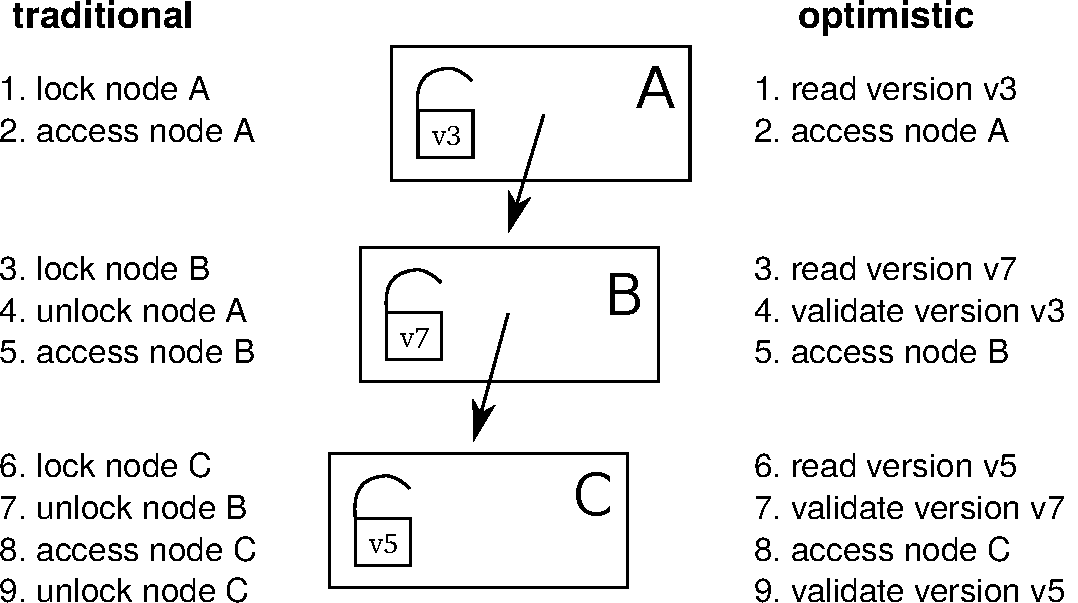
\includegraphics[width=0.65\linewidth]{olcall.pdf}
  \vspace{0.2cm}
  \caption{Comparison of a lookup operation in a 3-level tree using traditional lock coupling (left-hand side) vs.~optimistic lock coupling (right-hand side).}
  \label{fig:olc}
\end{figure}

The traditional and most common lock-based synchronization protocol for B-trees is lock coupling, which interleaves lock acquisitions while holding at most two locks at a time.
If, as we observed earlier, optimistic locks have similar semantics as traditional locks, it is natural to ask whether lock coupling can be combined with optimistic locks.
And indeed the answer is yes: One can almost mechanically translate traditional lock coupling code to optimistic lock coupling code.
This is illustrated in Figure~\ref{fig:olc}, which compares the traversal in a tree of height 3 using traditional and optimistic locks.
As the figure shows, the main difference is that locking is translated to reading the version and that unlocking becomes validation of the previously read version.
This simple change provides efficient lock-free tree traversal without the need to design a complex synchronization protocol.

It is important to emphasize the conceptual simplicity of OLC in comparison to data structures that use custom protocols like the Bw-tree~\cite{DBLP:conf/icde/LevandoskiLS13a}.
To implement lock-free access, the Bw-tree requires an indirection table, delta nodes, complex splitting and merging logic, retry logic, etc.
OLC, on the other hand, can directly be applied to B-trees mostly by adding the appropriate optimistic locking code and without modifying the node layout itself.
Therefore, OpenBw-Tree, an open source implementation of the Bw-tree, requires an order of magnitude more code than a B-tree based on OLC\footnote{Both implementations are available on GitHub: \url{https://github.com/wangziqi2016/index-microbench}}.
Given how difficult it is to develop, validate, and debug lock-free code, simplicity is obviously a major advantage.

\subsection{Correctness Aspects}

\begin{figure}
  % \centering
  %[basicstyle=\normalsize\ttfamily,showstringspaces=false,columns=fullflexible,breaklines=false,breakatwhitespace=true,numbers=none,numberstyle=\small,style=C,keepspaces=true]
\begin{lstlisting}[basicstyle=\ttfamily,language=C++,numbers=left,numberstyle=\small]
std::atomic<BTreeNode*> root;

// search for key in B+tree, returns payload in resultOut
bool lookup(Key key, Value& resultOut) {
   BTreeNode* node = root.load();
   uint64_t nodeVersion = node->readLockOrRestart();
   if (node != root.load()) // make sure the root is still the root
      restart();

   BTreeInner<Key>* parent = nullptr;
   uint64_t parentVersion = 0;

   while (node->isInner()) {
      auto inner = (BTreeInner*)node;

      // unlock parent and make current node the parent
      if (parent)
         parent->readUnlockOrRestart(parentVersion);
      parent = inner;
      parentVersion = nodeVersion;

      // search for next node
      node = inner->findChild(key);
      // validate 'inner' to ensure that 'node' pointer is valid
      inner->checkOrRestart(nodeVersion);
      // now it safe to dereference 'node' pointer (read its version)
      nodeVersion = node->readLockOrRestart();
   }

   // search in leaf and retrieve payload
   auto leaf = (BTreeLeaf*)node;
   bool success = leaf->findValue(key, resultOut);

   // unlock everything
   if (parent)
      parent->readUnlockOrRestart(parentVersion);
   node->readUnlockOrRestart(nodeVersion);

   return success;
}
\end{lstlisting}
  \vspace{0.2cm}
  \caption{B-tree lookup code using OLC. For simplicity, the restart logic is not shown.}
  \label{fig:lookup}
\end{figure}

So far, we have introduced the high-level ideas behind OLC and have stressed its similarity to traditional lock coupling.
Let us now discuss some cases where the close similarity between lock coupling and OLC breaks down.
To make this more concrete, we show the B-tree lookup code in Figure~\ref{fig:lookup}.
In the code, \texttt{readLockOrRestart} reads the lock version and \texttt{readUnlockOrRestart} validates that the read was correct.

One issue with OLC is that any pointer speculatively read from a node may point to invalid memory (if that node is modified concurrently).
Dereferencing such a pointer (e.g., to read its optimistic lock), may cause a segmentation fault or undefined behavior.
In the code shown in Figure~\ref{fig:lookup}, this problem is prevented by the extra check in line 25, which ensures that the read from the node containing the pointer was correct.
Without this additional validation, the code would in line 27 dereference the pointer speculatively read in line 23.
Note that the implementation of \texttt{checkOrRestart} is actually identical to \texttt{readUnlockOrRestart}.
We chose to give it a different name to highlight the fact that this extra check would not be necessary with read/write locks.

Another potential issue with optimistic locks is code that does not terminate.
Code that speculatively accesses a node, like an intra-node binary search, should be written in a way such that it always terminates---even in the presence of concurrent writes.
Otherwise, the validation code that detects the concurrent write will never run.
The binary search of a B-tree, for example, needs to be written in such a way that each comparison makes progress.
For some data structures that do not require loops in the traversal code (like ART) termination is trivially true.

\subsection{Implementation Details}

% implementation, efficiency
To implement an optimistic lock, one can combine the lock and the version counter into a single 64-bit\footnote{Even after subtracting one bit for the lock status, a back-of-the-envelope calculation can show that 63 bits are large enough to never overflow in practice.} word~\cite{artsync}.
A typical read operation will therefore merely consist of reading this version counter atomically.
In C++11 this can be implemented using the \texttt{std::atomic} type.

On x86, atomic reads are cheap because of x86's strong memory order guarantees.
No memory fences are required for sequentially-consistent loads, which are translated (by both GCC and clang) into standard \texttt{MOV} instructions.
Hence, the only effect of \texttt{std::atomic} for loads is preventing instruction re-ordering.
This makes version access and validation cheap.
Acquiring and releasing an optimistic lock in exclusive mode has comparable cost to a traditional lock:
A fairly expensive sequentially-consistent store is needed for acquiring a lock, while a standard \texttt{MOV} suffices for releasing it.
A simple sinlock-based implementation of optimistic locks can be found in the appendix of an earlier paper~\cite{artsync}.

OLC code must be able to handle restarts since validation or lock upgrade can fail due to concurrent writers.
Restarts can easily be implemented by wrapping the data structure operation in a loop (for simplicity not shown in Figure~\ref{fig:lookup}).
Such a loop also enables limiting the number of optimistic retry operations and falling back to pessimistic locking in cases of very heavy contention.
The ability to fall back to traditional locking is a major advantage of OLC in terms of robustness over lock-free approaches, which do not have this option.

In addition to the optimistic shared mode and the exclusive mode, optimistic locks also support a ``shared pessimistic'' mode, which physically acquires the lock in shared mode (allowing multiple concurrent readers but no writers).
This mode is useful for table (or range) scans that touch many tuples on a leaf page (which would otherwise easily abort).
Finally, let us mention that large range scans and table scans, should be broken up into several per-node traversals as is done in the LeanStore~\cite{leanstore} system.

Like all lock-free data structures, but unlike traditional locking and Hardware Transactional Memory~\cite{DBLP:conf/hpca/KarnagelDRLLSL14,DBLP:journals/pvldb/MakreshanskiLS15,htmtkde}, OLC requires care when deleting (and reusing) nodes.
The reason is that a deleting thread can never be sure that a node can be reclaimed because other threads might still be optimistically reading from that node.
Therefore, standard solutions like epoch-based reclamation~\cite{DBLP:conf/sosp/TuZKLM13}, hazard pointers~\cite{DBLP:journals/tpds/Michael04}, or optimized hazard pointers~\cite{DBLP:conf/spaa/BalmauGHZ16} need to be used.
These memory reclamation techniques are, however, largely orthogonal to the synchronization protocol itself.

%-lock-free is not a strong guarantee

\newpage
\section{Evaluation}\label{sec:evaluation}

Let us now experimentally evaluate the overhead and scalability of OLC.
For the experiments, we use an in-memory B+tree implemented in C++11 using templates, which is configured to use nodes of 4096 bytes, random 8 byte keys, and 8 byte payloads.
Based on this B-tree, we compare the following synchronization approaches:
\begin{itemize}
\item an OLC implementation\footnote{An almost identical OLC implementation is available on github: \url{https://github.com/wangziqi2016/index-microbench/tree/master/BTreeOLC}}
\item a variant based on traditional lock coupling and read/write locks
\item the unsynchronized B-tree, which obviously is only correct for read-only workloads but allows measuring the overhead of synchronization
\end{itemize}
Note that earlier work has compared the OLC implementation with a Bw-tree implementation~\cite{buzzword} and other state-of-the-art in-memory index structures.

We use a Haswell EP system with an Intel Xeon E5-2687W v3 CPU, which has 10 cores (20 ``Hyper-Threads'') and 25~MB of L3 cache.
The system is running Ubuntu 18.10 and we use GCC 8.2.0 to compile our code.
The CPU counters are obtained using the Linux perf API\footnote{We use the following convenience wrapper: \url{https://github.com/viktorleis/perfevent}}.

\begin{table}
  \caption{Performance and CPU counters for lookup and insert operations in a B-tree with 100M keys. We perform 100M operations and normalize the CPU counters by that number.}
  \label{tab:overhead}
  \centering
  \begin{tabular}{lrrrrrrr}\toprule
                    &         &        &        & instruc-  & L1     & L3     & branch \\
                    & threads & M op/s & cycles & tions & misses & misses & misses \\\midrule
lookup (no sync.)   & 1       & 1.72   & 2028   & 283     & 39.1   & 14.9   & 16.1   \\
lookup (OLC)        & 1       & 1.65   & 2107   & 370     & 43.9   & 15.1   & 16.7   \\
lookup (lock coup.) & 1       & 1.72   & 2078   & 365     & 42.3   & 16.9   & 15.7   \\\midrule
insert (no sync.)   & 1       & 1.51   & 2286   & 530     & 59.8   & 31.1   & 17.3   \\
insert (OLC)        & 1       & 1.50   & 2303   & 629     & 61.2   & 31.1   & 16.5   \\
insert (lock coup.) & 1       & 1.41   & 2473   & 644     & 61.0   & 31.0   & 17.2   \\\midrule
lookup (no sync.)   & 10      & 15.48  & 2058   & 283     & 38.6   & 15.5   & 16.0   \\
lookup (OLC)        & 10      & 14.60  & 2187   & 370     & 43.8   & 15.8   & 16.8   \\
lookup (lock coup.) & 10      & 5.71   & 5591   & 379     & 54.2   & 17.0   & 14.8   \\\midrule
insert (no sync.)   & 10      & -      & -      & -       & -      & -      & -      \\
insert (OLC)        & 10      & 10.46  & 2940   & 656     & 62.0   & 32.5   & 16.8   \\
insert (lock coup.) & 10      & 7.55   & 4161   & 667     & 75.0   & 28.6   & 16.2   \\
    \bottomrule
\end{tabular}
\end{table}

Table~\ref{tab:overhead} compares the performance and CPU counters for lookup and insert operations in a B-tree with 100M keys.
With {\em single-threaded} execution, we observe that all three approaches have very similar performance.
Adding traditional or optimistic locks to unsynchronized B-tree code results in up to 30\% of additional instructions without affecting single-threaded performance much.

\begin{figure}
  \centering
  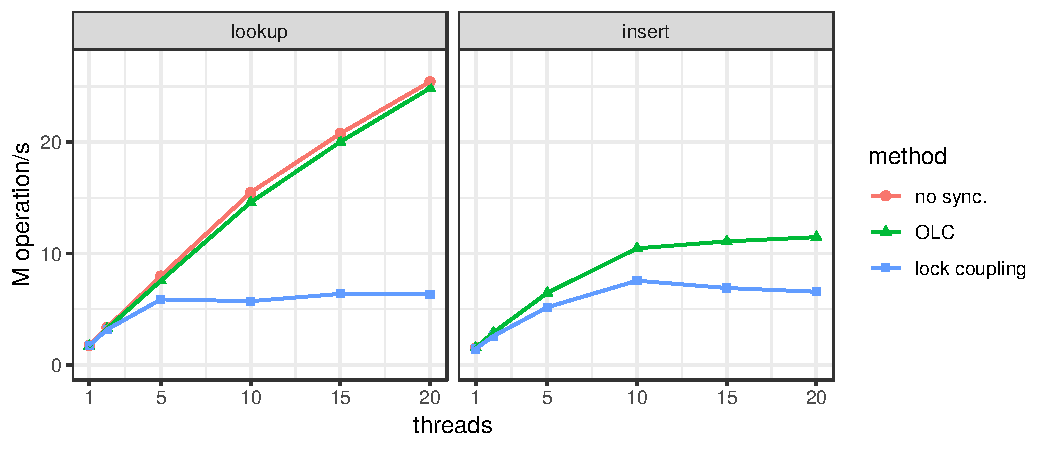
\includegraphics[width=\linewidth]{scale.pdf}
  \vspace{0.2cm}
  \caption{Scalability on 10-core system for B-tree operations (100M values).}
  \label{fig:scale}
\end{figure}

As Figure~\ref{fig:scale} shows, the results change dramatically once we use multiple threads.
For lookup, the scalability of OLC is near-linear up to 20 threads, even though the system has only 10 ``real cores''.
The OLC scalability for insert is also respectable (though not quite as linear because multi-threaded insertion approaches the memory bandwidth of our processor).
The figure also shows that the results of traditional lock coupling with read/write locks are significantly worse than OLC.
With 20 threads, lookup with OLC is 3.9$\times$ faster than traditional lock coupling.

\section{Summary}\label{sec:conc}

Optimistic Lock Coupling (OLC) is an effective synchronization method that combines the simplicity of traditional lock coupling with the superior scalability of lock-free approaches.
OLC is widely applicable and has already been successfully used to synchronize several data structures, including B-trees, binary search trees, and different trie variants.
These features make it highly attractive for modern database systems as well as performance-critical systems software in general.

\begin{thebibliography}{10}

\bibitem{DBLP:conf/spaa/BalmauGHZ16}
O.~Balmau, R.~Guerraoui, M.~Herlihy, and I.~Zablotchi.
\newblock Fast and robust memory reclamation for concurrent data structures.
\newblock In {\em SPAA}, 2016.

\bibitem{DBLP:journals/acta/BayerS77}
R.~Bayer and M.~Schkolnick.
\newblock Concurrency of operations on {B}-trees.
\newblock {\em Acta Informatica}, 9, 1977.

\bibitem{hot}
R.~Binna, E.~Zangerle, M.~Pichl, G.~Specht, and V.~Leis.
\newblock {HOT}: A height optimized trie index for main-memory database
  systems.
\newblock In {\em SIGMOD}, 2018.

\bibitem{DBLP:conf/ppopp/BronsonCCO10}
N.~G. Bronson, J.~Casper, H.~Chafi, and K.~Olukotun.
\newblock A practical concurrent binary search tree.
\newblock In {\em PPOPP}, 2010.

\bibitem{DBLP:conf/vldb/ChaHKK01}
S.~K. Cha, S.~Hwang, K.~Kim, and K.~Kwon.
\newblock Cache-conscious concurrency control of main-memory indexes on
  shared-memory multiprocessor systems.
\newblock In {\em VLDB}, 2001.

\bibitem{intel}
I.~Cutress.
\newblock {Intel} goes for 48-cores: {Cascade-AP} with multi-chip package
  coming soon.
\newblock
  \url{https://www.anandtech.com/show/13535/intel-goes-for-48cores-cascade-ap},
  2018 (accessed January, 2019).

\bibitem{DBLP:conf/cidr/FaleiroA17}
J.~M. Faleiro and D.~J. Abadi.
\newblock Latch-free synchronization in database systems: Silver bullet or
  fool's gold?
\newblock In {\em CIDR}, 2017.

\bibitem{DBLP:journals/ftdb/Graefe11}
G.~Graefe.
\newblock Modern {B}-tree techniques.
\newblock {\em Foundations and Trends in Databases}, 3(4), 2011.

\bibitem{DBLP:conf/hpca/KarnagelDRLLSL14}
T.~Karnagel, R.~Dementiev, R.~Rajwar, K.~Lai, T.~Legler, B.~Schlegel, and
  W.~Lehner.
\newblock Improving in-memory database index performance with
  {Intel}\({}^{\mbox{{\textregistered}}}\) transactional synchronization
  extensions.
\newblock In {\em HPCA}, 2014.

\bibitem{DBLP:journals/tods/LehmanY81}
P.~L. Lehman and S.~B. Yao.
\newblock Efficient locking for concurrent operations on {B}-trees.
\newblock {\em {ACM} Trans. Database Syst.}, 6(4), 1981.

\bibitem{leanstore}
V.~Leis, M.~Haubenschild, A.~Kemper, and T.~Neumann.
\newblock Leanstore: In-memory data management beyond main memory.
\newblock In {\em ICDE}, 2018.

\bibitem{art}
V.~Leis, A.~Kemper, and T.~Neumann.
\newblock The adaptive radix tree: {ARTful} indexing for main-memory databases.
\newblock In {\em ICDE}, 2013.

\bibitem{htmtkde}
V.~Leis, A.~Kemper, and T.~Neumann.
\newblock Scaling {HTM}-supported database transactions to many cores.
\newblock {\em {IEEE} Trans. Knowl. Data Eng.}, 28(2), 2016.

\bibitem{artsync}
V.~Leis, F.~Scheibner, A.~Kemper, and T.~Neumann.
\newblock The {ART} of practical synchronization.
\newblock In {\em DaMoN}, 2016.

\bibitem{DBLP:conf/icde/LevandoskiLS13a}
J.~J. Levandoski, D.~B. Lomet, and S.~Sengupta.
\newblock The {Bw}-tree: A {B}-tree for new hardware platforms.
\newblock In {\em ICDE}, 2013.

\bibitem{DBLP:journals/pvldb/MakreshanskiLS15}
D.~Makreshanski, J.~J. Levandoski, and R.~Stutsman.
\newblock To lock, swap, or elide: On the interplay of hardware transactional
  memory and lock-free indexing.
\newblock {\em {PVLDB}}, 8(11), 2015.

\bibitem{DBLP:dblp_conf/eurosys/MaoKM12}
Y.~Mao, E.~Kohler, and R.~T. Morris.
\newblock Cache craftiness for fast multicore key-value storage.
\newblock In {\em EuroSys}, 2012.

\bibitem{DBLP:journals/tpds/Michael04}
M.~M. Michael.
\newblock Hazard pointers: Safe memory reclamation for lock-free objects.
\newblock {\em {IEEE} Trans. Parallel Distrib. Syst.}, 15(6), 2004.

\bibitem{DBLP:journals/jacm/ShalevS06}
O.~Shalev and N.~Shavit.
\newblock Split-ordered lists: Lock-free extensible hash tables.
\newblock {\em J. {ACM}}, 53(3), 2006.

\bibitem{amd}
A.~Shilov.
\newblock {AMD} previews {EPYC} ‘{Rome}’ processor: Up to 64 {Zen} 2 cores.
\newblock
  \url{https://www.anandtech.com/show/13561/amd-previews-epyc-rome-processor-up-to-64-zen-2-cores},
  2018 (accessed January, 2019).

\bibitem{DBLP:conf/sosp/TuZKLM13}
S.~Tu, W.~Zheng, E.~Kohler, B.~Liskov, and S.~Madden.
\newblock Speedy transactions in multicore in-memory databases.
\newblock In {\em SOSP}, 2013.

\bibitem{buzzword}
Z.~Wang, A.~Pavlo, H.~Lim, V.~Leis, H.~Zhang, M.~Kaminsky, and D.~Andersen.
\newblock Building a {Bw}-tree takes more than just buzz words.
\newblock In {\em SIGMOD}, 2018.

\end{thebibliography}


%\bibliographystyle{abbrv}
%\bibliography{main}

\end{document}

\end{article}

\begin{article}
{Building Deletion-Compliant Data Systems}
{Manos Athanassoulis, Subhadeep Sarkar, Tarikul Islam Papon, Zichen Zhu, Dimitris Staratzis}
\graphicspath{{submissions/building-deletion-compliant-data-systems/}}
\documentclass[11pt,dvipdfmx]{article}


\usepackage{deauthor,times,graphicx}
\usepackage{booktabs} 
\usepackage{amsmath}
\usepackage{epstopdf}
\usepackage{verbatimbox}
\usepackage{multirow} 

%\graphicspath{{athanassoulis/}}


\newcommand\Paragraph[1]{\vspace{0.02in}  \noindent \textbf{#1.}}
\newcommand\Paragraphqit[1]{\vspace{0.02in}  \noindent \textit{#1?}}
\newcommand\Paragraphbit[1]{\vspace{0.02in}  \noindent \textbf{\textit{#1.}}}

\begin{document}



\title{Building Deletion-Compliant Data Systems}


\author{
Manos Athanassoulis, Subhadeep Sarkar, Tarikul Islam Papon, Zichen Zhu, Dimitris Staratzis
\medskip\\
Boston University
}



\maketitle


\begin{abstract}
Most modern data systems have been designed with two goals in mind -- fast ingestion and 
low-latency query processing. The first goal has led to the development of a plethora of 
write-optimized data stores that employ the \textit{out-of-place} paradigm. 
Due to their write-optimized design, out-of-place data systems perform deletes 
\textit{logically} via invalidation, and retain the invalid data for arbitrarily long. 
However, due to the recent enactment of new data privacy regulations, 
the requirement of \textit{timely deletion of user data} has become central. 
% One primary focus of privacy regulations is to establish the user's 
The \textit{right to be 
forgotten} (in EU's GDPR), \textit{right to delete} (in California's CCPA and CPRA), or 
\textit{deletion right} (in Virginia's VCDPA) mandates that service providers persistently delete a user's data within a pre-set time duration. 
Logical deletion in out-of-place data systems, however, does not offer guarantees for 
\textit{timely and persistent deletion}, and attempting to enforce it using existing tools 
leads to poor performance and increased operational costs. 

\hspace{0.02in} In this paper, we present a new framework for building \textit{deletion-compliant
data systems} from a holistic perspective. We analyze the new regulations and the 
requirements derived from the new policies, and we propose changes in the application and
the system layer of data management. We outline the new types of deletion requests that need to be supported, the query language
modifications needed to be able to request for timely persistent data deletion, and the system-level 
changes needed to realize timely and persistent deletes. 
The proposed framework for deletion compliance lays the groundwork for a new class of data 
systems that can offer system-level guarantees for user data privacy. We present recent results 
spanning all layers of the framework: the requirements and
the application layer target any database system, while the system layer discussion is geared 
towards out-of-place systems. Finally, we conclude with a discussion on next steps
and open challenges on building deletion-compliant data systems.

\end{abstract}





\section{Introduction}
\label{sec:introduction}


Data-intensive social and commercial applications and new advancements in domains like Internet-of-things, edge computing, 5G communications, and autonomous vehicles, generate a vast amount of \textit{personal data} processed by several data companies~\cite{Cisco2018,Gartner2017}. 
The increasing demand for efficient collection, storage, and processing of user data over the past two decades, has driven the development of data systems that can \textit{sustain high ingestion rates} without compromising the ability to \textit{access and analyze the data quickly}. 

\newpage
\Paragraph{Out-of-Place Systems}
The need for optimizing data ingestion while maintaining efficient data access has led
to the prominence of the \textit{out-of-place} paradigm, which fulfills these goals by
minimizing the interference between reads and writes. Today, several commercial relational and 
array-based data 
stores~\cite{Athanassoulis2011,Deng2020,Farber2012,Heman2010,Idreos2012,Kang2016,Lamb2012,Sadoghi2016,Stonebraker2005} and NoSQL data 
stores~\cite{ApacheAccumulo,ApacheCassandra,ApacheHBase,DeCandia2007,FacebookRocksDB,Golan-Gueta2015,Huang2019,Sears2012} have adopted the out-of-place paradigm. 

\textit{Relational and Array-based Systems}. 
Relational systems that buffer updates before applying them lazily on the base data, essentially, follow the out-of-place paradigm. 
The columnar and array data stores implemented by Vertica~\cite{Lamb2012,Stonebraker2005}, 
SciDB~\cite{Paradigm4,Stonebraker2013}, and TileDB~\cite{Papadopoulos2016,TileDB} use an in-memory storage component that stores incoming inserts, updates, and deletes out of place, and 
applies the changes lazily on the disk-resident data. Similarly, the state-of-the-art column-store system
MonetDB~\cite{Idreos2012} uses an in-memory positional index for incoming 
data~\cite{Heman2010}, and SAP HANA uses
a delta store per table to facilitate fast ingestion without affecting its 
read-optimized data layout~\cite{Farber2012}. 
Finally, several research-prototype systems
use a separate delta store on faster storage (e.g., SSDs/NVM) to 
offer efficient access to incoming 
data \cite{Athanassoulis2011,Athanassoulis2015,Deng2020,Kang2016,Sadoghi2016}.

\textit{NoSQL Systems}.
More than relational systems, production-grade NoSQL key-value stores predominantly employ the 
out-of-place paradigm, frequently based on the log-structured merge (LSM) paradigm.
An LSM-tree is a heavily write-optimized out-of-place data structure that maintains several on-disk components, which can be viewed as several out-of-place delta stores~\cite{ONeil1996,Dayan2017,Idreos2019,Luo2020b,Sarkar2022b,Zheng2018}.
Key-value stores such as RocksDB~\cite{Dong2017,FacebookRocksDB} and  LevelDB~\cite{GoogleLevelDB} at Facebook, BigTable~\cite{Chang2006} at Google, X-Engine~\cite{Huang2019,Yang2020} at Alibaba, Voldemort~\cite{LinkedInVoldemort} at LinkedIn, DynamoDB~\cite{DeCandia2007} at Amazon, Cassandra~\cite{ApacheCassandra}, HBase~\cite{ApacheHBase}, and Accumulo~\cite{ApacheAccumulo} at Apache, and bLSM~\cite{Sears2012} and cLSM~\cite{Golan-Gueta2015} at Yahoo are based on the log-structured merge (LSM) paradigm. 
Other out-of-place architectures employed by NoSQL systems are B$^+$-tree, B$^\epsilon$-tree, and fractal tree-based storage engines with \emph{buffering support}, such as COLA~\cite{Bender2000}, TokuDB~\cite{Kuszmaul2014}, and 
B\textit{e}rtFS~\cite{Bender2015,Jannen2015}. 

\textit{Cloud-based Systems}.
Cloud-based systems naturally employ the out-of-place paradigm as they rely on the 
immutability of cloud storage. Hence, systems like Amazon 
Redshift~\cite{AmazonRedshift,Gupta2015}, Cloud Data Platform~\cite{Dageville2016} at 
Snowflake, and Delta Lake~\cite{Databricks,Databricks2021} at Databricks employ variations
of the out-of-place paradigm in the interest of performance. 
Deletes and updates are initially performed logically and are gradually propagated to 
persistent media through periodic merging with base data. 

\Paragraph{Deletes in Out-of-Place Systems}
A key property of out-of-place systems is that they treat deletes (and updates) similarly to 
inserts, i.e., instead of deleting (updating) entries in-place, they insert a new version of 
the entry to be deleted that \textit{logically invalidates} the target entries. 
These special entries that are responsible for logical deletes are termed \textit{delete 
markers}~\cite{Lamb2012} or \textit{tombstones}~\cite{Dong2017,Sarkar2020}. 

Logical data deletion is a quintessential out-of-place operation, but it does not guarantee 
\emph{purging} of the data under deletion within a definite timeframe. Rather, the data is marked as
invalid; essentially, \emph{not accessible} to external users. In practice, logically 
deleted entries are kept for arbitrarily long in the system, since the time to definitively 
delete the data (termed \emph{persistent deletion}) depends on the state of the system, 
and not on when the user request expects the data to be deleted~\cite{Sarkar2020}.
In fact, most out-of-place data stores are built with the underlying assumption of 
\textit{perpetual data retention} in order to gain more insights from the user and 
organizational data~\cite{Whittaker2019}, hence \emph{timely persistent deletion} has not
been part of their design goals. In addition to deletes, logical updates in out-of-place 
systems are applied lazily too, however, the implications of out-of-place deletes are 
critical in terms of the privacy regulations, and thus, are our focus. 

\subsection{Problem: The Privacy Concern}
\Paragraph{Cost of Logical Deletes} Logical deletes and updates in out-of-place systems boost ingestion performance, however, they come at a significant cost.  
In fact, when tasked with deleting user data persistently in a timely manner, out-of-place systems suffer both in terms of (a) data privacy protection and (b) the overall system performance. 
Such systems are designed to retain the logically invalidated data indefinitely, and the time required for persistent removal of the physical data entries depends on (i) the data layout, (ii) the data re-organization policy (e.g., node splitting/merging in B-trees, compaction in LSM-trees, consolidation in TileDB), (iii) the design of the storage engine (such as the fanout of a tree and the size of a database), and (iv) the composition and distribution of the workload -- factors that are \textit{beyond the control of the application and system developers or administrators}. 
Thus, most out-of-place systems are unable to provide any latency guarantees for persistent deletion of user data~\cite{Sarkar2020}. 


\Paragraph{The Legal Frontier}
In recent years, a number of government-driven efforts across the globe unfolded, 
aiming to protect the privacy of user data and give back to the users the control of their 
personal data. On the legal side, regulations such as the EU's GDPR~\cite{GDPR}, California's 
CCPA~\cite{CCPA2018} and CPRA~\cite{CPRA}, and Virginia's 
VCDPA~\cite{VCPDA} have been introduced, which mandate that data companies ensure \textit{privacy through deletion}~\cite{Shastri2019,Shastri2021}. 
GDPR's \textit{right to be forgotten}, CCPA and CPRA's \textit{right to delete}, and the \textit{deletion right} in VCDPA particularly focus on \textit{persistent deletion of user data on-demand and in a timely manner}~\cite{Ambrose2013,Deshpande2018,Goddard2017,Jones2012,Sarkar2018,Shastri2019,Schwarzkopf2019,Tsesis2014}. 

\Paragraph{The Technological Roadblock} Treating \emph{deletes} as \textit{first-class citizens} is new for the data systems community, and it would require a significant amount of work to transform classical systems to be efficient deletion-wise. 
Even today, it continues to be a critical technological challenge for the biggest of data companies using state-of-the-art storage engines to demonstrate compliance with the deletion regulations and to efficiently delete user data on-demand~\cite{Shah2019,Shastri2020,Shastri2021}. 
To translate this into numbers, between January 2020 and January 2022, the penalties under GDPR paid by data companies amounted to more than \$1B, which includes large contributions from companies such as Amazon (\$877M), WhatsApp (\$255M), Google Ireland (\$102M), and Facebook (\$68M), H\&M (\$41M), British Airways (\$26M), and Marriot (\$23M)~\cite{Piper2022,DLAPiper2020,Tessian2022}. 
Thus, to demonstrate compliance, many companies end up performing expensive database-wide consolidations periodically (e.g., every few weeks), to ensure timely persistent deletion of user data~\cite{Sarkar2020,Sarkar2021c}. 
Such operations are remarkably expensive in terms of time and money, cause undesirable latency spikes, and hence, should be avoided. 

\begin{figure*}[tb]
    \centering
        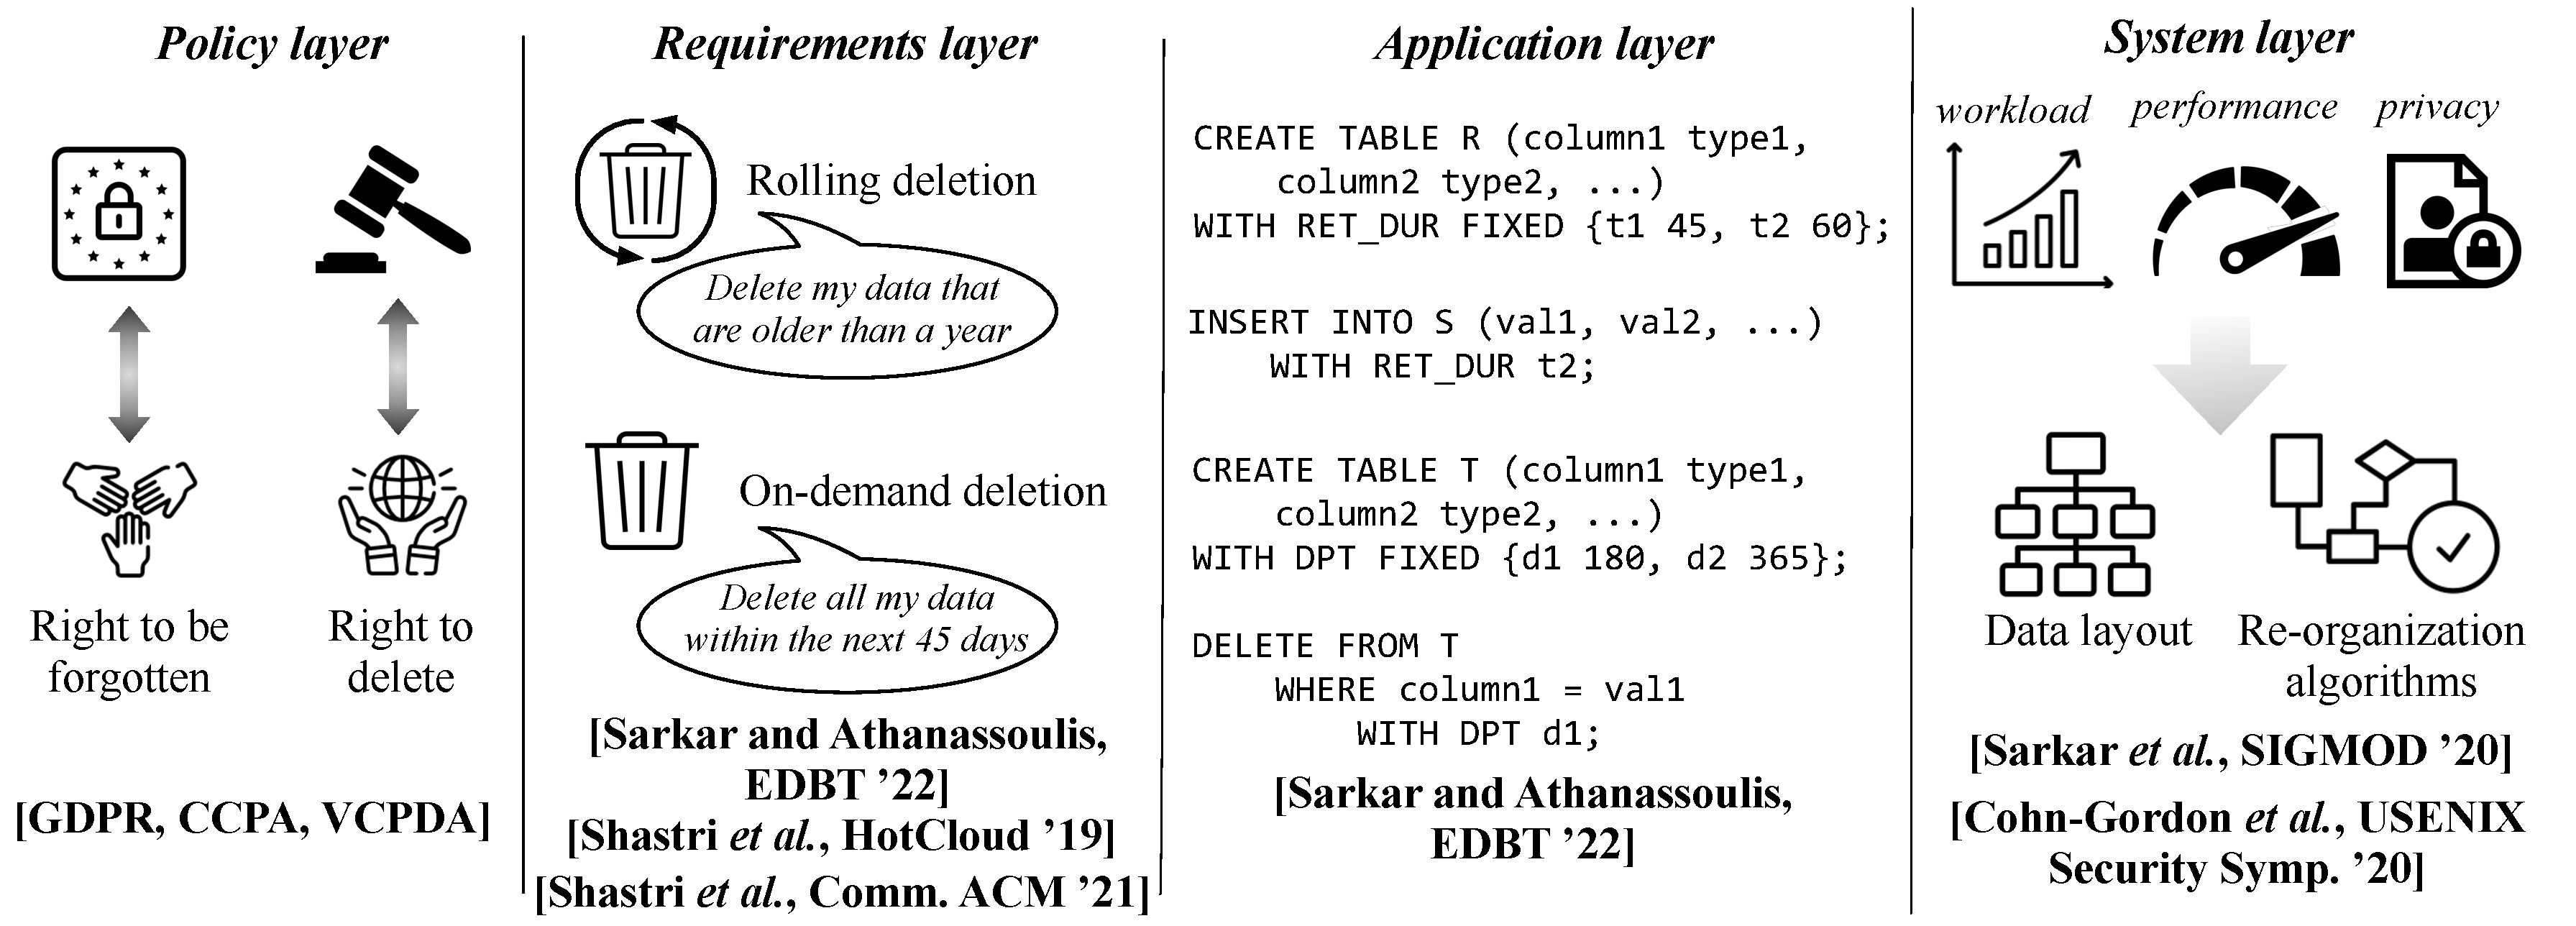
\includegraphics[scale=0.29]{figs/layered_problem_scenario.pdf}
    \vspace{-0.25in} 
    \caption{The four layers of deletion-compliant data systems.}
     \vspace{-0.1in}
    \label{fig: vision}
\end{figure*}

 
\subsection{Deletion-Compliant Data Systems}
In this paper, we present our vision and first results on designing data systems that ensure data privacy through timely and persistent deletion of user data. 
Existing efforts that attempt to delete user/application data on-demand suffer in terms of performance as the underlying data layout and data management mechanisms are ill-suited for the purpose. 
We identify the missing links, in terms of technological tools, both at the application level and the system level, and we propose a hierarchical framework that enables our vision of privacy through deletion in out-of-place data systems (Figure~\ref{fig: vision}).



\newpage
\Paragraph{Roadmap} 
The privacy through deletion framework is a roadmap toward building deletion-compliant data systems. 
We begin by outlining the challenges associated with each layer of our vision, i.e., in the context of (i)~translating the legal mandates to user requirements, (ii) expressing the user requirements through a declarative API, and (iii) realizing the application-level requirements at the system level.
Next, we identify and categorize the different classes of user requests for deletes in light of the legal regulations. 
Based on this, we present the challenges associated with transforming the classes of deletion requests into application-level specifications, and we propose an SQL extension as an example that can be extended to other query languages to support deletion of user data \textit{periodically} and \textit{on-demand}. 
Further, we outline the design and tools necessary at the system level to support the application-level requirements. 
Finally, we conclude with a discussion on how the proposed framework drives us toward building deletion-compliant data systems, and what further research challenges remain open to fully realize this vision.






%
 
\section{From Regulation to Practice}
\label{sec:legal}


The legal landscape for data privacy has changed drastically over the past few years, and governments across countries, as well as across different states in the US, have enforced acts and regulations to control the consumption of user data by service providers and give back to the users the control of their personal data. 
Translating the new regulations to new \emph{user-data privacy-compliant system behavior}
still faces significant challenges. In this section, we present in more detail the 
requirements from the regulation point of view, and we showcase through three realistic
scenarios the limitations of the state-of-the-art data systems when tasked to implement
these requirements. 


\subsection{Regulations on Timely Data Deletion}
While the new regulations propose an array of new requirements, we particularly focus on the legal 
policies concerning data retention and data deletion, with the objective of ensuring 
\textit{privacy through deletion}. 

\Paragraph{Right to be Forgotten, \textit{EU GDPR}}
The General Data Protection Regulation (GDPR) has revolutionized the data privacy and security landscape across the European Union countries~\cite{GDPR}. 
One of the fundamental changes introduced through the GDPR (over the older Data Protection Act (DPA) that it replaced), is the \textit{right to be forgotten}, which empowers the users with the \emph{right} to request a service provider to delete all their personal data persistently from its domain. 
Such deletion requests may be presented either up-front or on-demand. 
The service provider must comply with those requests, unless it has compelling reasons for acting otherwise (Art. 17(3)). 


\Paragraph{Right to Delete, \textit{CCPA}, \textit{CPRA}}
The California Customer Protection Act (CCPA), which will eventually be replaced by the California Privacy Rights Act (CPRA) in 2023, allows the users/consumers in California to request from service providers to permanently delete all data personal to the user~\cite{CCPA2018,CPRA}. 
Under CCPA and CPRA, the service providers must acknowledge such a user request within $10$ days, and respond to the request within $45$ business days~\cite{Brown2021}. 
Persistent deletion must be performed by removing the target data across all domains, barring archive and backup systems, along with data anonymization as required. 

\Paragraph{Right to Delete, \textit{VCDPA}}
Similarly to CCPA, the Virginia Consumer Data Protection Act (VCDPA) empowers users in Virginia to exercise their right to delete their personal data from a provider's domain~\cite{VCPDA}. 
VCDPA requires the service providers to serve a delete-request from a user within $45$ business days~\cite{Brown2021}. 


\Paragraph{Right to be Forgotten, \textit{UK GDPR, DPA}} 
The UK GDPR, along with the Data Protection Act (DPA) 2018 provides the country's citizens with similar rights about personal data deletion as the EU GDPR. 
The users are allowed to express their deletion preference verbally or in writing, to which the service providers must respond within $30$ days~\cite{UKGDPR,DPA2018}. 



\Paragraph{Other Efforts}  
Among other countries, Argentina~\cite{Carter2013,Pardo2020}, Singapore~\cite{Chik2013}, India~\cite{Kittane2021}, Canada~\cite{PIPEDA2019}, and South Korea~\cite{Brown2016} have some implementation of the right to deletion as a part of their respective privacy protection acts.



\subsection{Limitations of the State of the Art} 
In light of the deletion regulations, we now present three real-life scenarios to highlight why state-of-the-art data systems are ill-equipped to support deletes efficiently without hurting performance. 
We do so by identifying the missing links in different hierarchical levels of the proposed privacy-through-deletion framework.
Below, we illustrate (i) that the users are unable to express their preferences about deleting their personal data, (ii) why it is difficult for application developers to support the deletion requests from the users, and (iii) why it is difficult to realize persistent deletes in a timely manner in live production servers.


\textit{Scenario 1}: \textit{Alice} is a user of a smart-home ecosystem, \textit{HomeComp}, which provides real-time services including video surveillance, remote temperature, and illumination control. 
\textit{Alice} enjoys the services of \textit{HomeComp}, but concerned about her personal data privacy, she wants \textit{HomeComp} to permanently delete all her data older than $30$ days on a rolling basis.  

\Paragraphqit{The problem}
Like most service providers, \textit{HomeComp}'s data model is built around the assumption of perpetual data retention; deletion of user data needs a human-in-the-loop that performs the necessary actions.
Thus, \textit{HomeComp} does not allow its user to request for rolling timestamp-based data deletion. 

\textit{Scenario 2}: \textit{StreamEra} is a company that provides real-time insights for data streams, and allows its users to request on-demand deletion of their personal data, as it is bound by the \emph{right to be forgotten}.
\textit{StreamEra} uses an SQL-based wrapper on top of its storage layer.

\Paragraphqit{The problem} 
While \textit{StreamEra} wants to serve its users by ensuring timely persistent deletion of their personal data, SQL does not provide support for such an operation.
Instead, the backend engineers implement the user-requested deletion functionality at the application level in an ad-hoc manner as it is not native to SQL.

\textit{Scenario 3}: A cloud-based online data analysis company \textit{ClouData}, stores user data using immutable files within its HTAP data store. 
\textit{ClouData} is bound by the \emph{right to be forgotten}, and thus, has to delete all user data that are older than $D$ days.

\Paragraphqit{The problem} As the data organization on disk is not based on the ingestion timestamp and aims to accelerate read queries, it uses the most frequently
queried attribute to partition. Hence, the objects qualifying for a timestamp-based
deletion may be dispersed within the data store. 
As in-place deletion is not supported due to immutability, state-of-the-art data stores periodically consolidate the entire data set to delete all invalid entries. 
Ensuring privacy via this approach is costly in terms of disk writes and overall accesses, and causes latency spikes leading to performance unpredictability. 

\Paragraph{Other Challenges of Logical Deletes} In addition to not complying with regulatory requirements, 
logical deletes may cause more hurdles. Specifically,
by retaining invalidated data (that should not be used anymore), a data company:

\begin{enumerate}
	\item Wastes storage space and energy on data that cannot exploit in any way. Further, data maintenance results in additional write amplification that wears off the underlying storage devices \cite{Athanassoulis2016}.
	\item Risks that a security leak will reveal user data that users expect to be deleted~\cite{Piper2022}.
	\item Hurts read performance, as its data management layer uses metadata and indexes for all data regardless of whether they are invalidated~\cite{Sarkar2020}.
\end{enumerate}






\newpage 
\section{Privacy Through Timely Deletion}
\label{sec:vision}


We now outline our vision toward developing deletion-aware data systems, which by design, are capable of \emph{deleting user data persistently, and in an efficient and timely manner}. 
Toward this, we introduce a new set of application level and system level tools that capture, transform, and realize the user-requirements for deletes. 

Figure~\ref{fig: vision} shows our four-layered approach. The first step is the
\textit{policy layer}, implemented by the governments, that enact specific clauses to protect
data privacy through deletion. The second layer is the \emph{requirements layer} that 
translates the regulations into application requirements. Next, we have the \emph{application
layer} that proposes the necessary changes in query languages to allow applications to
easily express their constraints. Finally, the \emph{system
layer} implements efficient means for data deletion and demonstrates regulation compliance.


\subsection{Requirements Layer}
\vspace{-0.05in}

\Paragraph{Challenge} 
This layer analyzes the regulations from the policy layer and categorizes the various requests the
user \emph{should be} able to make on the application layer. The impact of the newly enacted policies
is on various aspects including accountability (audit), security (protect data access), and right of access
(efficient accessing) \cite{Shah2019,Shastri2021}. In this work, we focus on \emph{storage limitation} 
(``data should not be stored beyond its purpose''), the \emph{right to be forgotten} (``find and
delete groups of data'')~\cite{Shah2019}, and how to transform them into concrete requirements.



\Paragraph{Types of Deletion Requests} 
We codify the two types of data deletion requests as requirements for (a)~retention-driven \emph{rolling 
deletion} and (b)~\emph{on-demand deletion} both with a timely constraint~\cite{Sarkar2020}, as illustrated 
in the second part of Figure~\ref{fig: vision}.

\Paragraphbit{Retention-driven deletes} 
In cases that the purpose of storing the data has expired, a rolling deletion should take place, which
will ensure that the underlying data management solutions persistently delete this data, based on a
pre-set \textit{retention duration}. This duration can be governed by legislation, the specific application,
or even user preference, hence it has to be tunable. To abide by the policies, the data management
layer has to permanently delete expired items within a specific timeframe, provided by the service-level
agreement (SLA) between the user and the service providers.

\Paragraphbit{Deletion on-demand} 
The regulations for deletes also allow users to submit on-demand deletion requests for any personal data,
upon which the service provider has to delete user data persistently. 
On-demand deletion requests can be submitted through an API provided by the service provider, and upon 
submission, all data for a user are purged persistently within a threshold period. 
This threshold for persistent deletion is also set by the provider following the regulations and is 
agreed upon in the form of an SLA-clause. 


\subsection{Application Layer}
\vspace{-0.05in}

\Paragraph{Challenge} With the deletion-related regulations translated to deletion requirements, the next step 
is to transform them into a format that is interpretable by the application layer. The interface of
data stores is typically declarative query languages (e.g., SQL, GraphQL, DMX, LINQ, and N1QL) that support expressing complex queries as well as
inserting new data, updates, and deletes. The missing link here
is that state-of-the-art query languages do not have support for data deletion based on retention and
does not have a way to express the timely deletion requirements. 


\Paragraph{Extending SQL}
Hence, to implement the deletion requirements, we propose an extension to SQL~\cite{Sarkar2022} that includes
support for timely deletion both in the data definition (DDL) and the data 
manipulation (DML) parts of the language, as summarized in the third part of 
Figure~\ref{fig: vision}. 
The objective of the SQL extension is three-fold. 

\begin{itemize} \vspace*{-0.5mm}
	\item[1.] To support \textit{retention-driven deletion}, we augment both the \texttt{CREATE TABLE} and \texttt{INSERT INTO} statements so that a relational table can be associated with a number of options for specific time-to-live (TTL). Every data object is bound to a specific TTL according to the application SLA or to user preference. 
	\item[2.] To ensure \textit{timely persistence of on-demand deletion requests}, we augment the \texttt{CREATE TABLE} and \texttt{DELETE FROM} statements to allow a relational table to support a predetermined set of timely deletion guarantees, and each deletion to select the level of service to which it adheres.
	\item[3.] Finally, we extend the \texttt{CREATE TABLE}, \texttt{INSERT INTO} and \texttt{DELETE FROM} statements to support \emph{arbitrary delete thresholds} for retention duration and deletion persistence.
\end{itemize}

 


\Paragraphbit{Enabling retention-driven deletes}
To support retention-driven deletes, we extend \texttt{CREATE TABLE} to allow an
application developer to specify several levels of retention duration as a table property.

\begin{verbnobox}[\fontsize{9pt}{10pt}\selectfont]
    CREATE TABLE R (column1 type1, column2 type2, ...) 
    WITH RET_DUR FIXED (t1 <ret1>, t2 <ret2>, ...);
\end{verbnobox}
The above \texttt{CREATE TABLE} statement creates a table \texttt{R} that supports 
retention-based deletes with specific retention duration of \texttt{ret1}, 
\texttt{ret2}, etc, which are mapped to symbolic representations \texttt{t1}, 
\texttt{t2}, etc.
In general, the \texttt{WITH RET\_DUR} clause is an optional clause when creating
a new table, and will be necessary only for tables that need to support deletes with 
predefined retention duration values. In such cases, each \texttt{INSERT} statement can use 
(up to) one of the predefined retention duration values, say \texttt{t1} to classify the 
specific object as one to be deleted after \texttt{ret1} time.
For example, a table that is configured to support retention duration of 30 days and 60 days (\texttt{CREATE TABLE R (...) WITH RET\_DUR FIXED (t1 '30 days', t2 '60 days');}), 
can only receive inserts with retention duration \texttt{t1} or \texttt{t2}.
An ingestion without a retention period explicitly mentioned, is kept perpetually 
following the logic of a classical insert. 
The syntax of an insert, now, has the 
optional \texttt{WITH RET\_DUR} clause as follows.
\begin{verbnobox}[\fontsize{9pt}{10pt}\selectfont]
 INSERT INTO R (val1, val2, ...) WITH RET_DUR t<i>;
\end{verbnobox}


\Paragraphbit{Support for arbitrary retention duration}
To support arbitrary retention duration, we further add the \texttt{ARBITRARY} 
keyword to both the \texttt{CREATE TABLE} and \texttt{INSERT} statements.
The support for arbitrary retention duration is necessary particularly for systems
in a distributed setting that replicate data across physical data stores in different 
geolocations, each bound by different regulatory requirements. 
The full syntax of the proposed SQL extension for retention-based deletion is below.
\begin{verbnobox}[\fontsize{9pt}{10pt}\selectfont]
 CREATE TABLE R (column1 type1, column2 type2, ...) 
 WITH RET_DUR {ARBITRARY | FIXED (t1 <ret1>, t2 <ret2>, ...)};
\end{verbnobox}
\begin{verbnobox}[\fontsize{9pt}{10pt}\selectfont]
 INSERT INTO R (val1, val2, ...) WITH RET_DUR { <t> | t<i> } ;
\end{verbnobox} 
Note that having a \emph{pre-defined set of retention duration values} provides more 
information to the system compared to allowing arbitrary duration. As a result, it 
\emph{allows the system to better prepare} to offer efficient retention-driven 
deletes. Conversely, we expect that data stores that aim to support arbitrary 
retention duration will face increased system-level challenges.


\Paragraphbit{Enabling timely on-demand deletion}
We further propose to augment SQL to express timely on-demand deletion. To do so, 
we introduce the concept of \textit{delete persistence threshold} 
(DPT)~\cite{Sarkar2020}, which denotes the maximum delay between a logical delete and 
its persistence. Every relational table can be associated with several such thresholds
that are defined from the legal constraints or based on user preference.
Similarly to retention-driven deletes, we also extend SQL to support arbitrary DPTs 
when the DPTs are not specified \textit{a priori}. 
Below, we outline the modifications to the DDL and DML parts of SQL to support on-demand timely deletion requests.
\begin{verbnobox}[\fontsize{9pt}{10pt}\selectfont]
 CREATE TABLE S (column1 type1, column2 type2, ...) 
 WITH DPT {ARBITRARY | FIXED (d1 <dpt1>, d2 <dpt2>, ...)};
\end{verbnobox}
\begin{verbnobox}[\fontsize{9pt}{10pt}\selectfont]
 DELETE FROM S WHERE (...) WITH DPT { <d> | d<i> };
\end{verbnobox}
Table \texttt{S} can support several DPTs (e.g., \texttt{dpt1}, \texttt{dpt2}) as long 
as the DPTs are pre-determined. Applications can trigger on-demand deletion 
with any such DPT through the \texttt{DELETE} command. 
Similarly to retention-driven deletes, timely persistent deletion of data on-demand is easier to handle from a storage engine if the DPTs supported are known \textit{a priori} during the table creation.

\Paragraph{Putting everything together}
With the proposed SQL extensions, a relational table can now support multiple 
(pre-defined or arbitrary) thresholds for both retention-based and on-demand deletes, 
with the following \texttt{CREATE TABLE} statement. 
\begin{verbnobox}[\fontsize{9pt}{10pt}\selectfont]
 CREATE TABLE T (column1 type1, column2 type2, ...) 
 WITH RET_DUR {ARBITRARY | FIXED (t1 <ret1>, t2 <ret2>, ...)};
 WITH DPT {ARBITRARY | FIXED (d1 <dpt1>, d2 <dpt2>, ...)};
\end{verbnobox}
Note that typically retention-based deletes come from the \emph{application requirements},  and 
on-demand deletion requests are issued \emph{by the user}. However, in both cases,
the deletes have to happen \emph{timely} as per the regulatory requirements.
The proposed changes in SQL are not enough to guarantee that the system will deliver on the
need for timely and persistent data deletion. Rather, they create the interface for data systems so that
need for timely deletion. Rather, they create the interface for data systems so that
the users and applications can express the deletion requests which is enforced by the regulations. The data deletion \emph{per se} is realized at the \textit{system level}, and we will next discuss advances and challenges on that front.


\subsection{System Layer}
\label{subsec:system-level}

With the requirement analysis and the declarative interface in place, the users
and the applications can express all the mandated deletion requests and the
underlying system is now tasked with implementing them. Before discussing the 
challenges of implementing timely retention-based and on-demand deletes, we discuss
the taxonomy of system-level deletes the application layer may initiate. In other
words, we want to understand what delete patterns may be generated at the system
layer. 

\subsubsection{Taxonomy of Deletes at the System Layer}
The behavior of a low-level delete operation depends on (i) the logical organization 
and physical layout of the data, and (ii) the attribute based on which the deletion
requests are issued. To better understand this \emph{delete design space}, we
classify different delete operations across two dimensions: (a) deletes on 
\emph{primary} vs. \emph{secondary} attributes, and (b) deletes based
on a single value of the delete attribute, termed \emph{point deletes}, vs. 
deletes on a range of the delete attribute, termed \emph{range 
deletes}~\cite{Sarkar2020}.
Table \ref{tab:summary} summarizes the state of the art in out-of-place
systems for different delete operations, their performance impact, and their 
at-large implications.

\begin{table}[h]
    \centering
   {
   \scriptsize
        \begin{tabular}{c|cc|cc}
        \toprule
        \multicolumn{1}{c}{\multirow{2}{*}{\begin{tabular}[c]{@{}c@{}}\textbf{Delete Workloads} \end{tabular}}}  & \multicolumn{2}{c}{\textbf{Primary Deletes}}   & \multicolumn{2}{c}{\textbf{Secondary Deletes}}                    \\
        \multicolumn{1}{c}{}                                                                    & \multicolumn{1}{c}{Point}        & \multicolumn{1}{c}{Range}   & \multicolumn{1}{c}{Point}        & \multicolumn{1}{c}{Range}    \\
        \midrule        
        \multirow{1}{*}{State-of-the-art}     
            & \multirow{1}{*}{insert point tombstones}    
            & \multirow{1}{*}{insert range tombstones}        
            & \multirow{2}{*}{not supported}  
            & \multirow{2}{*}{full-tree compaction}         
        \\  implementation & (\textit{logical}) 
            & (\textit{logical}) 
            & 
            & \\
        \midrule        
        \multirow{1}{*}{Point query}     
            & \multirow{1}{*}{search for key; stop}    
            & \multirow{1}{*}{search for key; compare fetched key}        
            & \multirow{1}{*}{N/A}  
            & \multirow{1}{*}{N/A}         \\
            path
            & if a tombstone is found
            & with the histogram (discard if invalidated)
            &
            & \\
        \midrule        
        \multirow{1}{*}{Range query}     
            & \multirow{1}{*}{merge qualifying sorted runs;}    
            & \multirow{1}{*}{merge qualifying sorted runs;}        
            & \multirow{1}{*}{N/A}  
            & \multirow{1}{*}{N/A}         \\
            path
            & discard on the fly if TS exist
            & check each value against histogram
            & 
            & \\
        \midrule        
        \multirow{4}{*}{Implications}     
            & \multirow{1}{*}{unbounded persistence latency}    
            & \multirow{1}{*}{unbounded persistence latency}        
            & \multirow{1}{*}{}  
            & \multirow{1}{*}{huge latency spikes}         
        \\  & high space amplification 
            & high space amplification
            & N/A
            & high write amplification
        \\  & high write amplification
            & high write amplification
            & 
            & superfluous reads from disk
        \\  & 
            & severely affects read performance 
            & 
            & \\
        \bottomrule
        \end{tabular}
   }
   \vspace{-0.1in}
    \caption{Implications of logical deletes on performance in state-of-the-art out-of-place data stores.} \label{tab:summary}
    \vspace{-0.1in}
\end{table}

\Paragraph{Primary Deletes} In out-of-place systems, data is ultimately organized based on a so-called
\emph{sort key} (for example, the key of the key-value pairs in an LSM-tree). The
sort key often is the primary key of the database, hence, a majority of delete 
operations can be expressed as deletes based on the sort key, or \emph{primary
deletes}. Note that even deletes on other attributes may be preferable to be
converted to primary deletes if there is a secondary index. Both point and range
primary deletes use the notion of a \emph{delete marker} or a \emph{tombstone}
that is inserted in the data collection (on the deleted sort key) and invalidates 
prior version of the key(s), and they are very common in real workloads~\cite{Cao2020}. 
Primary deletes can be triggered either by user activity (i.e., on-demand) or by automated processes (e.g., data migration). 

\Paragraphbit{Implications and Challenges} When an out-of-place system has files that contain
tombstones, then both point and range query paths are affected. Specifically, since the system
accesses files with decreasing age (i.e., the most recent ones first) when 
looking for a key (\emph{point query}), it will also be looking for tombstones. If a 
tombstone is found,
the search will terminate because all other (older) instances of that key are 
invalid. 
In the presence of range deletes, the implementation is more complex as it is hard
to use per-file range delete tombstones~\cite{Madan2018}. Instead, a database-wide histogram
of deleted ranges is maintained and every query compares against this histogram before 
proceeding~\cite{Sarkar2020}.
When considering \emph{range queries}, all the sorted files have to be merged 
and the deleted entries are discarded on the fly by comparing against the
visited point and range tombstones~\cite{Callaghan2020}. 

The implications of primary deletes are multi-fold. First, while out-of-place 
systems support deletes, any deletion is logical, and there is no \emph{a priori}
bound on the delete persistence latency. Second, by maintaining both the tombstones
and the invalid entries for arbitrarily long time, the systems pay in terms of 
increased space amplification. Thirdly, by reorganizing data including invalid 
entries and tombstones, we further pay in terms of increased write amplification.
Note that space and write amplification \cite{Athanassoulis2016,Dong2017} are two 
fundamental sources of cost when deploying data system. Finally, while range 
tombstones are used to offer the range delete functionality, they are rather 
cumbersome and impact the read performance severely~\cite{Callaghan2020,Madan2018}.

\Paragraph{Secondary Deletes} In some other cases, we may need to organize data 
based on a sort key, but we have a majority of deletes on a different attribute.
Note that if we have individual deletes on a different attribute, the most 
prudent approach is to guarantee that we have a secondary index and transform a
secondary delete in one (or more) primary point delete, hence in
Table~\ref{tab:summary}, we see the lack of support for point secondary deletes.  
However, in some cases, we may have long range deletes on a secondary attribute. 
For example, when working on a window of the most recent data we can 
repetitively delete data based on a timestamp. A similar case is the 
retention-based deletes introduced earlier. 

\Paragraphbit{Implications and Challenges} Secondary range deletes are not 
native in out-of-place systems, since the underlying data is organized based on
the sort key. While converting them to a collection of point primary deletes might
work in several cases, it will overload the system with tombstones. Instead, 
several systems opt to perform a full-database merging and re-writing periodically
to fulfill any secondary range deletion constraints they might have to follow. This approach leads
to significant write amplification, superfluous data accesses, and a large 
penalty in terms of latency spikes on the workload during this merging.

\Paragraph{From Delete Requirements to Delete Types} The delete taxonomy at the
system level helps us map the delete requirements to low-level data operations. 
A retention-driven deletion is typically modeled as a secondary range delete, and
if the delete range has few objects (i.e., low selectivity), it can be implemented as a collection of
primary point deletes. On the other hand, on-demand deletion is typically 
implemented as a primary point or range delete and there are several performance 
challenges to be addressed.

\subsubsection{Realizing Timely Deletes}
Timely data deletion while respecting the retention SLAs without hurting the system 
performance is a key challenge. The efficiency of deletion depends on the schema and 
the physical data layout, the data re-organization strategy, the workload, and the 
design of the storage engine. The right-most part of Figure~\ref{fig: vision}
outlines the design changes needed and the input parameters used to co-optimize the 
performance of a storage engine while ensuring timely delete persistence. We
now discuss how both classes of deletes can be realized efficiently through 
modifications in the design of out-of-place storage engines, focusing on 
LSM-bases storage engines.

\Paragraph{Realizing Primary Deletes}
An LSM-based storage engine implements a primary delete by inserting a tombstone
on the desired key (or key-range) with a DPT associated. The application-provided
DPT is an indicator for how long a logical delete may live before its persistence,
that is, before purging any invalidated versions of the key(s) under deletion. The
tombstone representation is augmented with additional metadata, e.g., an extra byte 
to account for $128$ possible different DPTs in the same table. 
During its natural course of data re-organization the storage engine checks for any 
data blocks (i.e., pages, files, or sorted runs) with an expired TTL and 
consolidates them to ensure timely persistence. This data consolidation in LSM-based
data stores is called \emph{compaction}~\cite{Sarkar2022a,Sarkar2021c} and is the process of
selecting some components of the database (files, sorted runs) to merge and discard
invalid entries. At any point of time an LSM-based system has several files that 
may be compacted (it can be in the order of several thousands) so the decision which files to 
compact is a crucial decision. In general, the decision is based on read query 
metrics, however, in Lethe~\cite{Sarkar2020} we propose a new approach that 
prioritizes compactions of files depending on the age of the tombstones they contain.
Specifically, we assign different TTLs based on the level of the underlying LSM-tree 
and when there is a tombstone with an expired TTL we select the file that contains
it for compaction, as shown in Figure~\ref{fig:ec}. A key decision is how to ensure
that the multi-step merging of tombstones will always respect the 
application-defined DPT. This is ensured by assigning a different TTL to each 
tombstone after every compaction in a way that the sum of all its TTL amounts to the 
desired DPT. 


\begin{figure}[t]
    \centering  
        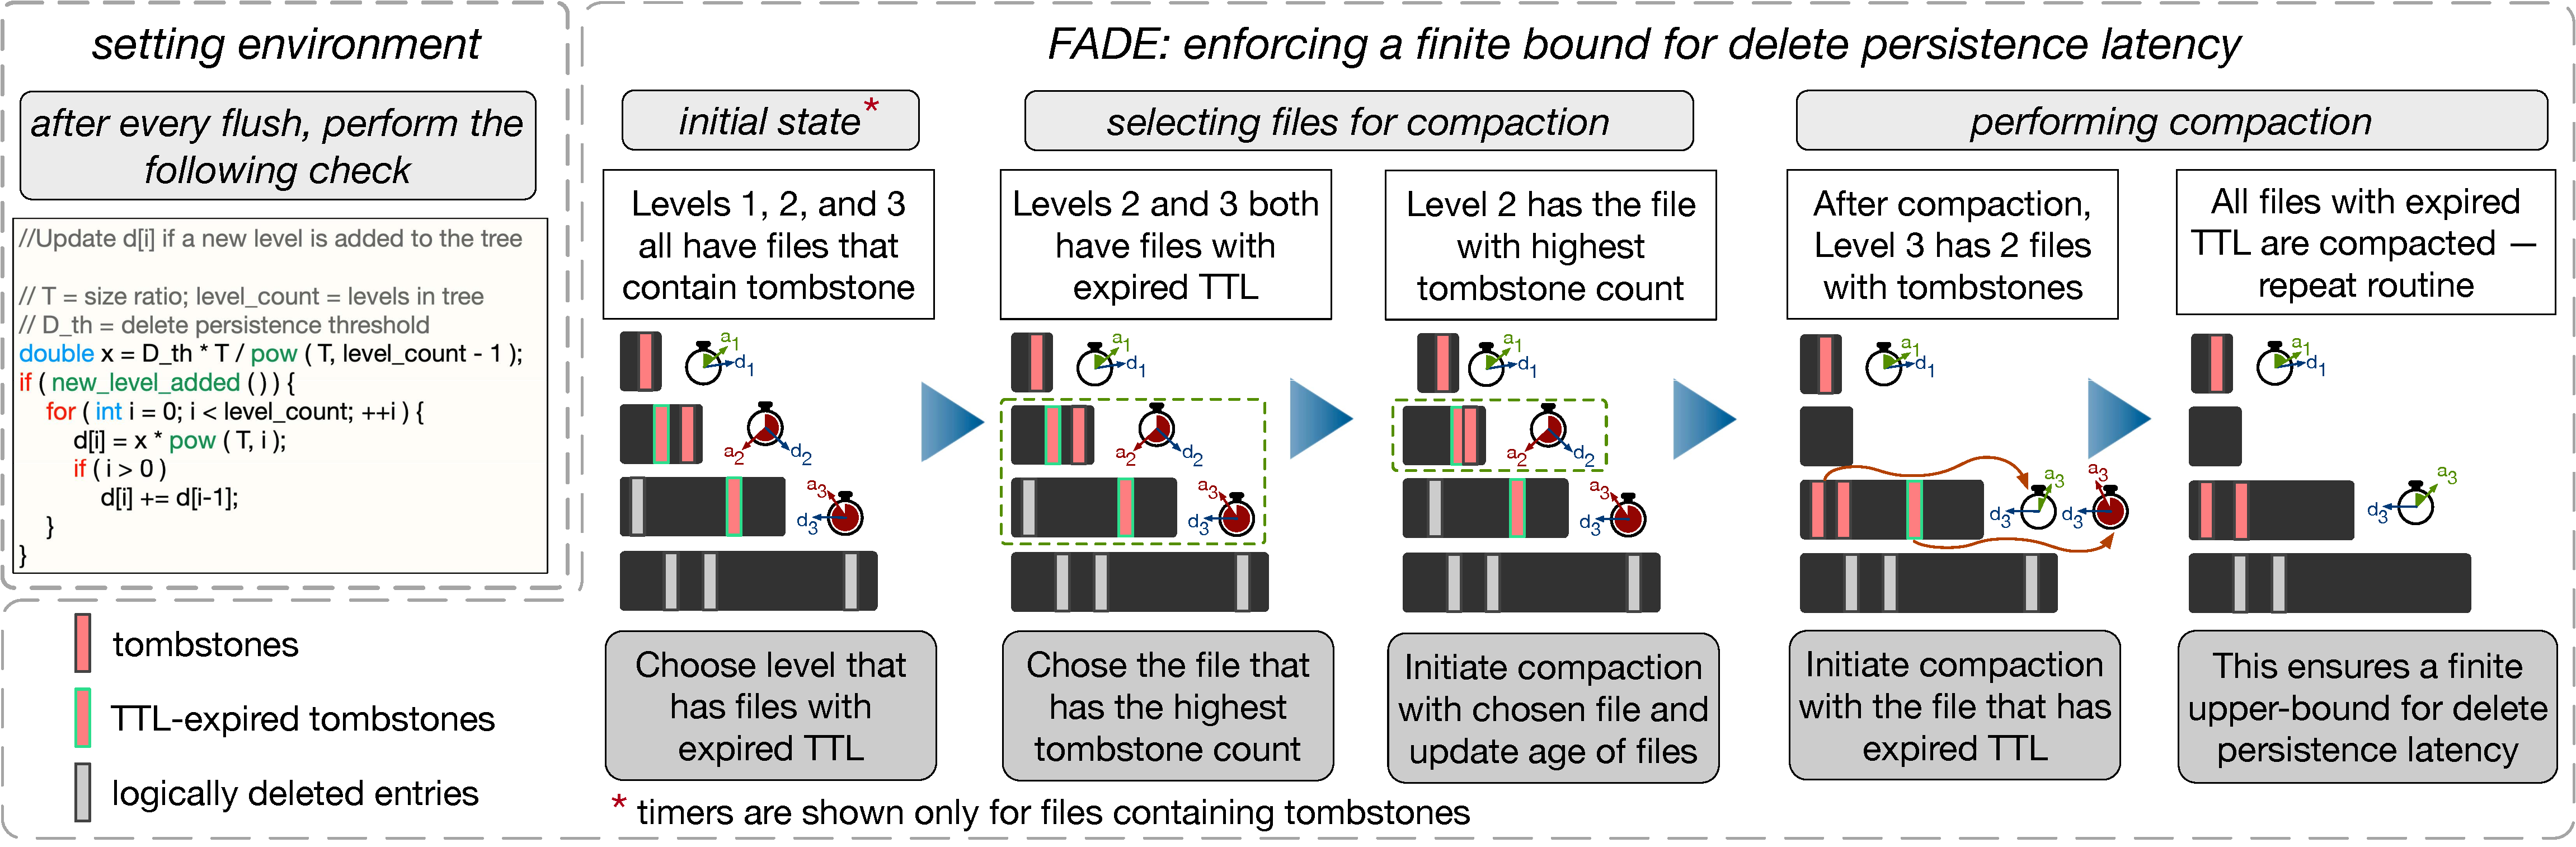
\includegraphics[width=\textwidth]{figs/effacingcompaction.pdf} 
        \vspace{-0.25in}        
    \caption{FADE persists tombstones within DPT, thus, improving overall performance.}
    \label{fig:ec} 
\vspace{0.2in}        
\end{figure} 

\begin{figure}[t]
    \centering  
        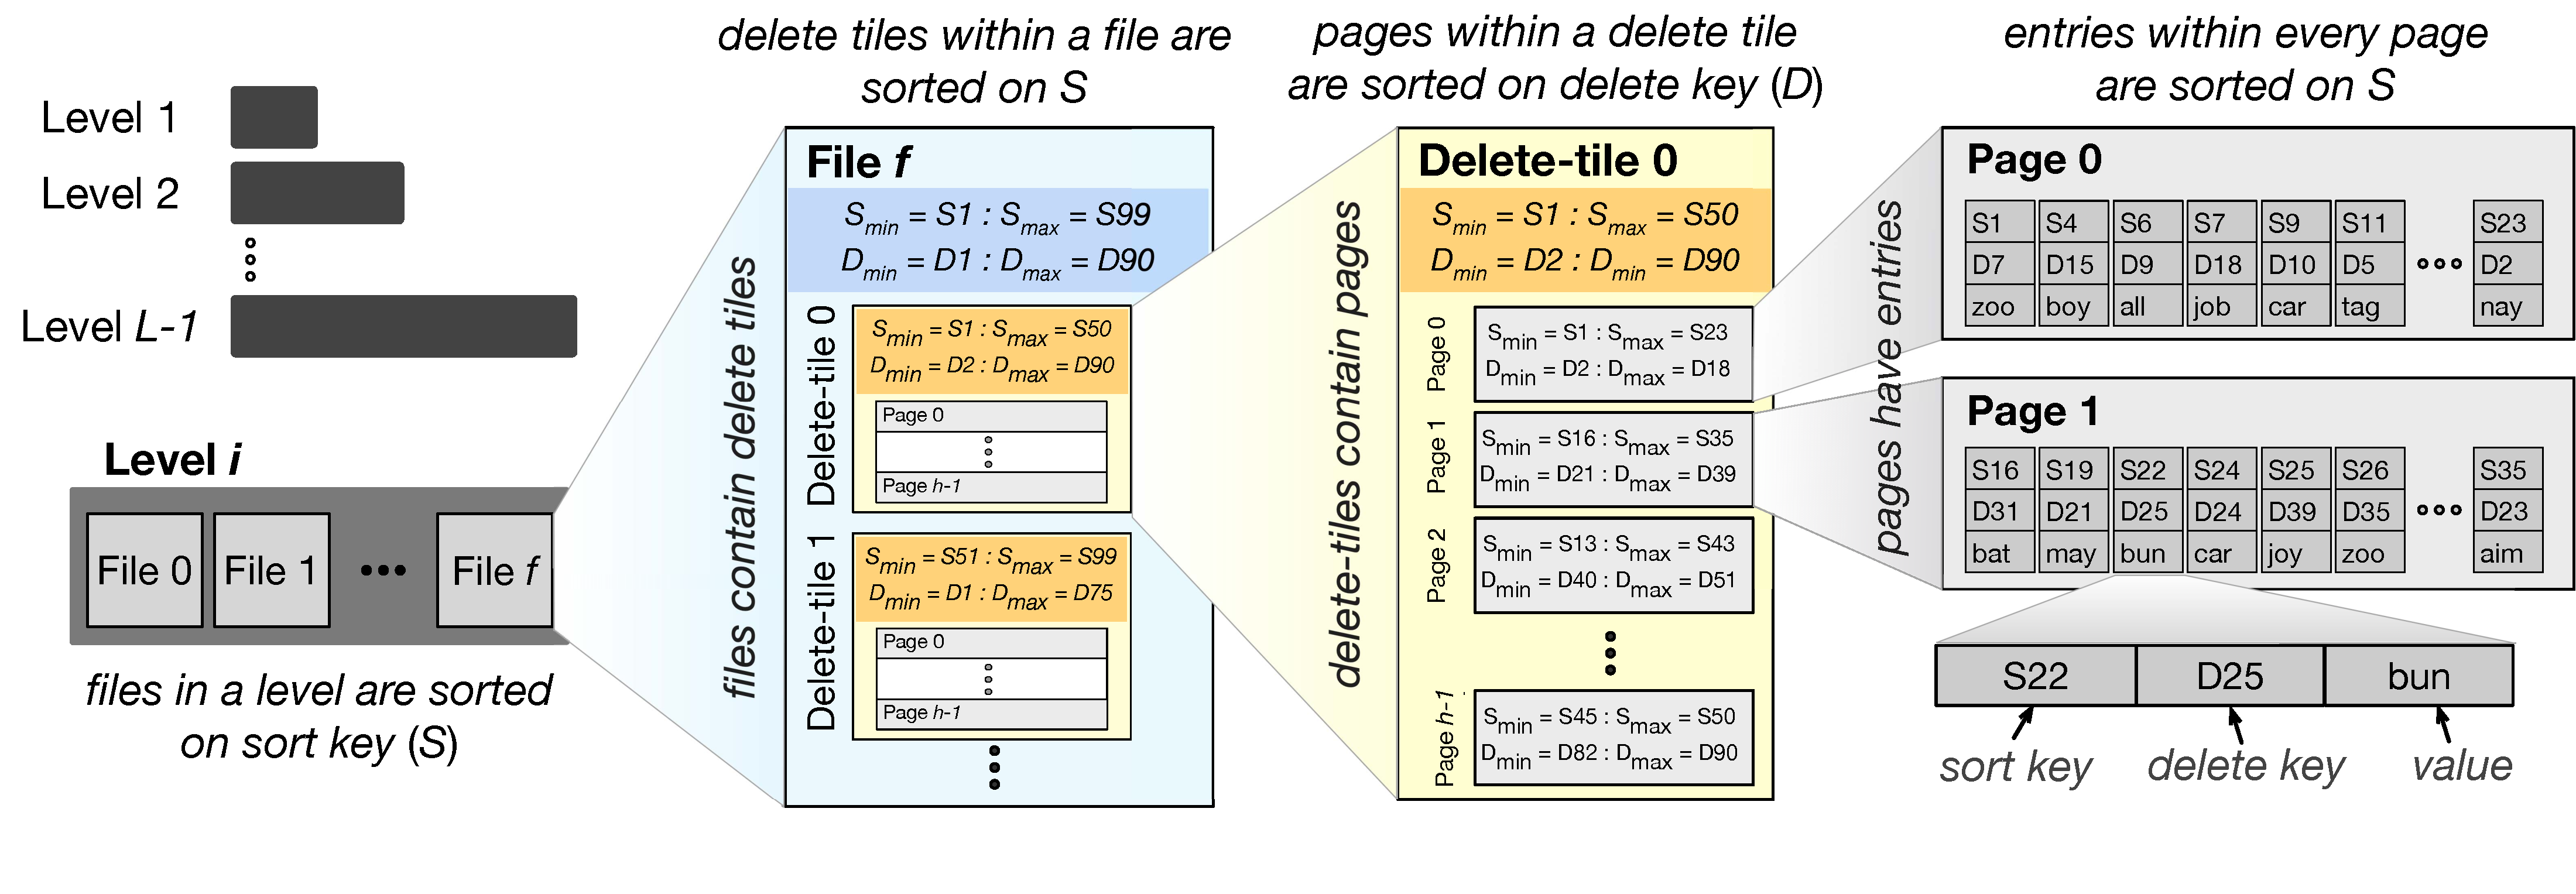
\includegraphics[width=\textwidth]{figs/storage_layout.pdf} 
   \vspace{-0.25in}        
    \caption{KiWi stores data in an interweaved fashion on the sort and delete key to facilitate efficient secondary range deletes while offering competitive  read performance.}
    \label{fig:layout} 
   \vspace{-0.15in}        
\end{figure} 


\Paragraph{Realizing Secondary Deletes}
As we discussed above, several instances of secondary deletes can be realized as
a collection of primary point deletes. However, when we are frequently tasked to
deleted a range of values based on a secondary attribute, we can achieve something
significantly better. In particular, a new weaved data layout between the original
sort key and the (secondary) delete key can offer much more efficient and timely
secondary range deletion while maintaining competitive read performance. The key idea is
to create a nested data organization that alternates between organizing data
based on the sort key (to facilitate good search performance) and based on the
delete key (to allow for consecutive chunks of data to be deleted at a time). 

This approach is implemented in the KiWi data layout~\cite{Sarkar2020} as shown in
Figure~\ref{fig:layout}. The core idea is that while the major components of the
database (files) are organized based on the sort key, every file is composed of
delete tiles that are internally organized based on the delete key,
partitioning the data accordingly. Lastly, each data page is again organized on
the search key to facilitate efficient in-memory search. The benefit for this
weaved data layout is that in the case of secondary range deletes, we can discard
entire groups of pages at a time, signaling the file system to reclaim this page
instantly, essentially converting the secondary delete to a page reclamation action
that has very low latency compared to a full database reorganization. In the 
worst case, we will have to in-place edit a few pages at the edge of the range, 
which is a tunable parameter that controls the maximum secondary deletion 
persistence latency as a tradeoff vs. read performance. 

\Paragraph{Evaluation} 
The approaches presented above for timely deletion were implemented as part of the
LSM-based system Lethe~\cite{Sarkar2020}, and achieved efficient timely
deletion respecting predetermined guarantees. The left hand-side of Figure~\ref{fig:results} shows the CDF of the 
tombstone age while varying the desired DPT to 16\%, 25\%, and 50\% of the duration
of the experiment. The colored areas correspond to the number of cumulative 
tombstones for the corresponding age on the x-axis, while the horizontal dotted-line
is the desired DPT. We observe that Lethe was able to always deliver the
requested DPT. The gray area corresponds to the age of tombstones of the state of
the art, where no DPT is imposed and deletes are not persisted timely. Notably, we also measured that enforcing the 
desired DPT shows benefits in terms of access time because the amount of invalid 
data was reduced. Similarly, we saw benefits in space amplification, and only marginal
cost increase in amortized write amplification.

The right hand-side of Figure~\ref{fig:results} shows the fraction of fully dropped
pages during a range delete as we vary the size of the delete tiles. We observe
that the fraction of pages fully dropped increases with the delete tile size, allowing
for efficient reclamation of the invalid data. Conversely, the read queries become
more expensive as we allow for more page drops, so the ideal delete tile size should
be tuned based on the workload. 


\begin{figure}[t]
    \centering  
        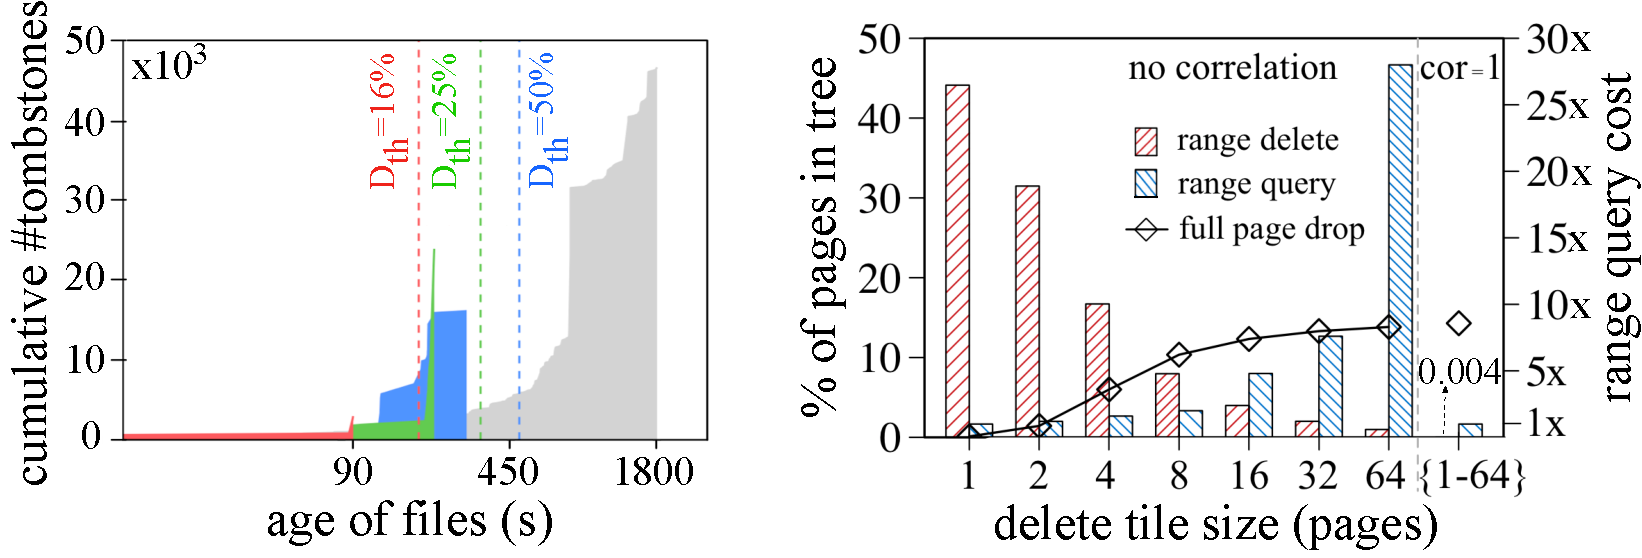
\includegraphics[width=\textwidth]{figs/lethe_figures.pdf} 
   \vspace{-0.25in}        
    \caption{Lethe ensures timely persistence of logically invalidated data within LSM-based out-of-place data systems for both primary and secondary classes of deletes.}
    \label{fig:results} 
   \vspace{-0.15in}        
\end{figure} 

\newpage
\Paragraph{Deletes in a Complex Data Model} The previous discussion focuses on
handling deletes in a per-instance manner without considering multiple copies of the
data in a more complex setting. Cohn-Gordon \textit{et al.}~\cite{Cohn-Gordon2020} proposed the deletion 
framework \textit{DELF} that ensures reliable data deletion from an online social 
network (OSN). 
\textit{DELF} enables detection of inconsistent data deletion in OSNs and also 
facilitates data recovery in cases where user data was incorrectly deleted. 
Minaei \textit{et al.}~\cite{Minaei2019} proposed a framework for persistently deleting all instances 
of user data in presence of observers, thereby, ensuring privacy through timely 
content concealment and removal. 





 
\section{Challenges and Opportunities}
\label{sec:challenges}
\vspace{-0.075in}



In Section~\ref{sec:vision}, we outlined the steps taken to realize the four-layered
vision of delete-compliant data systems presented in Figure~\ref{fig: vision}, 
however, there are still open questions and challenges for such systems which pose
opportunities for further innovative systems research.



\Paragraph{Device-level Deletion}
Data management solutions rely on storage devices and treat them as black boxes.
However, deleting data persistently at the device level and from data archives is an open 
technological challenge. Current endeavors in this direction are mainly focused on 
encryption-based solutions~\cite{Kissel2014,Koppel2013,Li2019a}.
Nevertheless, retention-based deletes entail persistent deletion of a ``quantum'' of data 
(e.g., the data ingested in a day) posing the following challenges for 
encryption-based solutions.
First, it is hard to \textit{determine the encryption granularity} while minimizing 
the encrypt/decrypt overhead. Second, with several data streams for different users/applications (and thus, bound by different SLAs), 
it is hard to \textit{manage the encryption keys efficiently and in a scalable manner}.
Third, efficient and scalable \textit{deletion from archives and backup stores on-demand} is hard to be supported by encryption-based deletion as the encrypt/decrypt cost and the fine encryption granularity adds prohibitive overheads.
Finally, from a legislation point-of-view it is not yet clear whether encrypting
and discarding the key is an accepted form of deletion.

When considering a system-level deletion similar approach to the one presented in 
Section~\ref{subsec:system-level} storage devices are essentially one more level of 
managing data at the physical layer and similar approaches have to be implemented
in the file system or the file and data systems have to be developed in tandem.

\Paragraph{Cloud-Level Deletion}
Further, operating on the cloud, data systems use virtualized devices and
object storage which is even more abstract hiding the details of how the 
low-level device and page management is taking place. Offering guarantees for
timely data deletion in virtualized storage will require a similar multi-layered
approach where the file system and the device firmware will expose knobs to allow
the application on top to request specific page reclamation properties. 





\Paragraph{Deletion in Distributed/Federated Computing Environment} 
With more and more data stores being transformed to cloud-based stores, user data 
may be collected, processed, and stored across multiple domains, spread across 
different geographic locations~\cite{Sarkar2018}. 
With different geographic locations being bound by different privacy regulations, we 
need to design \textit{solutions to ensure consistency for persistent deletion} of 
user data. 
Our intuition is that existing solutions for data stream-tainting~\cite{Enck2010}, 
cross-domain data tracing~\cite{Demsky2011,Herbster2016}, and related data 
provenance solutions~\cite{Buneman2018,Hasan2019} can be useful to address this 
problem.



\Paragraph{Compliance Demonstration} 
Last but certainly not least, data systems have to be able to prove compliance
when audited. The natural way to do so now is via log auditing, however, a more
light-weight algorithmic way for providing this will benefit both systems and users.
Inspecting logs and the underlying data is a time-consuming process and the 
long-term goal of the community should be to design system-level tools that can 
verifiably prove compliance with the privacy regulations. 
One interesting development in this direction is the evolution of security-driven 
operating systems, such as seL4~\cite{Klein2010,SeL4}. 
Another approach that can be taken is to show that the codebase of a data system
has the necessary code-paths for timely deletion via static and dynamic analysis.
An open challenge is to develop static and dynamic analysis tools that can prove
that a system deletes data respecting the timely deletion requirements set.









 
\section{Conclusion}
\label{sec:conclusion}
\vspace{-0.075in}

In this paper, we highlight that the recently enacted regulations  mandate
new data deletion requirements, requiring a new breed of data systems to support
them. We show that existing state-of-the-art out-of-place systems are ill-equipped
for this task, and we present a four-layered approach towards building the necessary
infrastructure. We present recent work on that front, and we conclude by discussing
several open research challenges.

\Paragraph{Acknowledgments} This work was partially funded by National
Science Foundation under Grant No. IIS-1850202 and a Facebook
Faculty Research Award.




 

\begin{thebibliography}{10}
\itemsep=1pt
\begin{small}


  \bibitem{UKGDPR}
  {Right to erasure}.
  \newblock {\em
    https://ico.org.uk/for-organisations/guide-to-data-protection/guide-to-the-general-data-protection-regulation-gdpr/individual-rights/right-to-erasure/}.
  
  \bibitem{GDPR}
  {Regulation (EU) 2016/679 of the European Parliament and of the council of 27
    April 2016 on the protection of natural persons with regard to the processing
    of personal data and on the free movement of such data, and repealing
    Directive 95/46/EC}.
  \newblock {\em Official Journal of the European Union (Legislative Acts)},
    pages L119/1 -- L119/88, 2016.
  
  \bibitem{CCPA2018}
  {California Consumer Privacy Act}.
  \newblock {\em Assembly Bill No. 375, Chapter 55}, 2018.
  
  \bibitem{DPA2018}
  {Data Protection Act 2018}.
  \newblock {\em
    https://www.legislation.gov.uk/ukpga/2018/12/pdfs/ukpga{\_}20180012{\_}en.pdf},
    2018.
  
  \bibitem{PIPEDA2019}
  {PIPEDA in brief}.
  \newblock {\em
    https://www.priv.gc.ca/en/privacy-topics/privacy-laws-in-canada/the-personal-information-protection-and-electronic-documents-act-pipeda/pipeda{\_}brief/},
    2019.
  
  \bibitem{CPRA}
  {The California Privacy Rights Act of 2020}.
  \newblock {\em https://thecpra.org/}, 2020.
  
  \bibitem{VCPDA}
  {Virginia Consumer Data Protection Act}.
  \newblock {\em
    https://www.sullcrom.com/files/upload/SC-Publication-Virginia-Second-State-Enact-Privacy-Legislation.pdf},
    2021.
  
  \bibitem{AmazonRedshift}
  Amazon.
  \newblock {Redshift}.
  \newblock {\em https://aws.amazon.com/redshift/}.
  
  \bibitem{Ambrose2013}
  M.~L. Ambrose and J.~Ausloos.
  \newblock {The Right to Be Forgotten Across the Pond}.
  \newblock {\em Journal of Information Policy}, 3:1--23, 2013.
  
  \bibitem{ApacheAccumulo}
  Apache.
  \newblock {Accumulo}.
  \newblock {\em https://accumulo.apache.org/}.
  
  \bibitem{ApacheHBase}
  Apache.
  \newblock {HBase}.
  \newblock {\em http://hbase.apache.org/}.
  
  \bibitem{ApacheCassandra}
  Apache.
  \newblock {Cassandra}.
  \newblock {\em http://cassandra.apache.org}, 2021.
  
  \bibitem{Athanassoulis2011}
  M.~Athanassoulis, S.~Chen, A.~Ailamaki, P.~B. Gibbons, and R.~Stoica.
  \newblock {MaSM: Efficient Online Updates in Data Warehouses}.
  \newblock In {\em Proceedings of the ACM SIGMOD International Conference on
    Management of Data}, pages 865--876, 2011.
  
  \bibitem{Athanassoulis2015}
  M.~Athanassoulis, S.~Chen, A.~Ailamaki, P.~B. Gibbons, and R.~Stoica.
  \newblock {Online Updates on Data Warehouses via Judicious Use of Solid-State
    Storage}.
  \newblock {\em ACM Transactions on Database Systems (TODS)}, 40(1), 2015.
  
  \bibitem{Athanassoulis2016}
  M.~Athanassoulis, M.~S. Kester, L.~M. Maas, R.~Stoica, S.~Idreos, A.~Ailamaki,
    and M.~Callaghan.
  \newblock {Designing Access Methods: The RUM Conjecture}.
  \newblock In {\em Proceedings of the International Conference on Extending
    Database Technology (EDBT)}, pages 461--466, 2016.
  
  \bibitem{Bender2000}
  M.~A. Bender, E.~D. Demaine, and M.~Farach-Colton.
  \newblock {Cache-Oblivious B-Trees}.
  \newblock In {\em Proceedings of the Annual Symposium on Foundations of
    Computer Science (FOCS)}, pages 399--409, 2000.
  
  \bibitem{Bender2015}
  M.~A. Bender, M.~Farach-Colton, W.~Jannen, R.~Johnson, B.~C. Kuszmaul, D.~E.
    Porter, J.~Yuan, and Y.~Zhan.
  \newblock {An Introduction to B$\epsilon$-trees and Write-Optimization}.
  \newblock {\em White Paper}, 2015.
  
  \bibitem{Brown2016}
  C.~T. Brown and T.~D. Manoranjan.
  \newblock {South Korea Releases Guidance on Right to Be Forgotten}.
  \newblock {\em
    https://www.lexology.com/library/detail.aspx?g=21be3837-0c43-4047-b8b5-9e863960b0b9},
    2016.
  
  \bibitem{Brown2021}
  G.~A. Brown.
  \newblock {Consumers' "Right to Delete" under US State Privacy Laws}.
  \newblock {\em
    https://www.securityprivacybytes.com/2021/03/consumers-right-to-delete-under-us-state-privacy-laws/},
    2021.
  
  \bibitem{Buneman2018}
  P.~Buneman and W.-C. Tan.
  \newblock {Data Provenance: What next?}
  \newblock {\em SIGMOD Rec.}, 47(3):5--16, 2018.
  
  \bibitem{Callaghan2020}
  M.~Callaghan.
  \newblock {Deletes are fast and slow in an LSM}.
  \newblock {\em
    http://smalldatum.blogspot.com/2020/01/deletes-are-fast-and-slow-in-lsm.html},
    2020.
  
  \bibitem{Cao2020}
  Z.~Cao, S.~Dong, S.~Vemuri, and D.~H.~C. Du.
  \newblock {Characterizing, Modeling, and Benchmarking RocksDB Key-Value
    Workloads at Facebook}.
  \newblock In {\em Proceedings of the USENIX Conference on File and Storage
    Technologies (FAST)}, pages 209--223, 2020.
  
  \bibitem{Carter2013}
  E.~L. Carter.
  \newblock {Argentina's Right to be Forgotten}.
  \newblock {\em Emory International Law Review}, 27(1), 2013.
  
  \bibitem{Chang2006}
  F.~Chang, J.~Dean, S.~Ghemawat, W.~C. Hsieh, D.~A. Wallach, M.~Burrows,
    T.~Chandra, A.~Fikes, and R.~E. Gruber.
  \newblock {Bigtable: A Distributed Storage System for Structured Data}.
  \newblock In {\em Proceedings of the USENIX Symposium on Operating Systems
    Design and Implementation (OSDI)}, pages 205--218, 2006.
  
  \bibitem{Chik2013}
  W.~B. Chik.
  \newblock {The Singapore Personal Data Protection Act and an assessment of
    future trends in data privacy reform}.
  \newblock {\em Comput. Law Secur. Rev.}, 29(5):554--575, 2013.
  
  \bibitem{Cisco2018}
  Cisco.
  \newblock {Cisco Global Cloud Index: Forecast and Methodology, 2016–2021}.
  \newblock {\em White Paper}, 2018.
  
  \bibitem{Cohn-Gordon2020}
  K.~Cohn-Gordon, G.~Damaskinos, D.~Neto, J.~Cordova, B.~Reitz, B.~Strahs,
    D.~Obenshain, P.~Pearce, I.~Papagiannis, and A.~Media.
  \newblock {DELF: Safeguarding deletion correctness in Online Social Networks}.
  \newblock In {\em 29th USENIX Security Symposium, USENIX Security 2020, August
    12-14, 2020}, 2020.
  
  \bibitem{Dageville2016}
  B.~Dageville, T.~Cruanes, M.~Zukowski, V.~Antonov, A.~Avanes, J.~Bock,
    J.~Claybaugh, D.~Engovatov, M.~Hentschel, J.~Huang, A.~W. Lee, A.~Motivala,
    A.~Q. Munir, S.~Pelley, P.~Povinec, G.~Rahn, S.~Triantafyllis, and
    P.~Unterbrunner.
  \newblock {The Snowflake Elastic Data Warehouse}.
  \newblock In {\em Proceedings of the ACM SIGMOD International Conference on
    Management of Data}, pages 215--226, 2016.
  
  \bibitem{Databricks}
  Databricks.
  \newblock {Online reference}.
  \newblock {\em https://databricks.com/}.
  
  \bibitem{Databricks2021}
  Databricks.
  \newblock {Table deletes, updates, and merges}.
  \newblock {\em
    https://docs.databricks.com/delta/delta-update.html{\#}delete-from-a-table},
    2021.
  
  \bibitem{Dayan2017}
  N.~Dayan, M.~Athanassoulis, and S.~Idreos.
  \newblock {Monkey: Optimal Navigable Key-Value Store}.
  \newblock In {\em Proceedings of the ACM SIGMOD International Conference on
    Management of Data}, pages 79--94, 2017.
  
  \bibitem{DeCandia2007}
  G.~DeCandia, D.~Hastorun, M.~Jampani, G.~Kakulapati, A.~Lakshman, A.~Pilchin,
    S.~Sivasubramanian, P.~Vosshall, and W.~Vogels.
  \newblock {Dynamo: Amazon's Highly Available Key-value Store}.
  \newblock {\em ACM SIGOPS Operating Systems Review}, 41(6):205--220, 2007.
  
  \bibitem{Demsky2011}
  B.~Demsky.
  \newblock {Cross-application data provenance and policy enforcement}.
  \newblock {\em ACM Transactions on Information Systems (TOIS)},
    14(1):6:1----6:22, 2011.
  
  \bibitem{Deng2020}
  F.~Deng, Q.~Cao, S.~Wang, S.~Liu, J.~Yao, Y.~Dong, and P.~Yang.
  \newblock {SeRW: Adaptively Separating Read and Write upon SSDs of Hybrid
    Storage Server in Clouds}.
  \newblock In {\em Proceedings of the International Conference on Parallel
    Processing (ICPP)}, pages 76:1----76:11, 2020.
  
  \bibitem{Deshpande2018}
  A.~Deshpande and A.~Machanavajjhala.
  \newblock {ACM SIGMOD Blog: Privacy Challenges in the Post-GDPR World: A Data
    Management Perspective}.
  \newblock {\em http://wp.sigmod.org/?p=2554}, 2018.
  
  \bibitem{Dong2017}
  S.~Dong, M.~Callaghan, L.~Galanis, D.~Borthakur, T.~Savor, and M.~Strum.
  \newblock {Optimizing Space Amplification in RocksDB}.
  \newblock In {\em Proceedings of the Biennial Conference on Innovative Data
    Systems Research (CIDR)}, 2017.
  
  \bibitem{Enck2010}
  W.~Enck, P.~Gilbert, B.-G. Chun, L.~P. Cox, J.~Jung, P.~D. McDaniel, and
    A.~Sheth.
  \newblock {TaintDroid: An Information-Flow Tracking System for Realtime Privacy
    Monitoring on Smartphones}.
  \newblock In {\em Proceedings of the USENIX Symposium on Operating Systems
    Design and Implementation (OSDI)}, pages 393--407, 2010.
  
  \bibitem{FacebookRocksDB}
  Facebook.
  \newblock {RocksDB}.
  \newblock {\em https://github.com/facebook/rocksdb}, 2021.
  
  \bibitem{Farber2012}
  F.~F{\"{a}}rber, N.~May, W.~Lehner, P.~Gro{\ss}e, I.~M{\"{u}}ller, H.~Rauhe,
    and J.~Dees.
  \newblock {The SAP HANA Database -- An Architecture Overview}.
  \newblock {\em IEEE Data Engineering Bulletin}, 35(1):28--33, 2012.
  
  \bibitem{Gartner2017}
  Gartner.
  \newblock {Gartner Says 8.4 Billion Connected ``Things" Will Be in Use in 2017,
    Up 31 Percent From 2016}.
  \newblock https://tinyurl.com/Gartner2020, 2017.
  
  \bibitem{Goddard2017}
  M.~Goddard.
  \newblock {The EU General Data Protection Regulation (GDPR): European
    Regulation that has a Global Impact}.
  \newblock {\em International Journal of Market Research}, 59(6):703--705, 2017.
  
  \bibitem{Golan-Gueta2015}
  G.~Golan-Gueta, E.~Bortnikov, E.~Hillel, and I.~Keidar.
  \newblock {Scaling Concurrent Log-Structured Data Stores}.
  \newblock In {\em Proceedings of the ACM European Conference on Computer
    Systems (EuroSys)}, pages 32:1--32:14, 2015.
  
  \bibitem{GoogleLevelDB}
  Google.
  \newblock {LevelDB}.
  \newblock {\em https://github.com/google/leveldb/}, 2021.
  
  \bibitem{Gupta2015}
  A.~Gupta, D.~Agarwal, D.~Tan, J.~Kulesza, R.~Pathak, S.~Stefani, and
    V.~Srinivasan.
  \newblock {Amazon Redshift and the Case for Simpler Data Warehouses}.
  \newblock In {\em Proceedings of the ACM SIGMOD International Conference on
    Management of Data}, pages 1917--1923, 2015.
  
  \bibitem{Hasan2019}
  S.~S. Hasan, N.~H. Sultan, and F.~A. Barbhuiya.
  \newblock {Cloud Data Provenance using IPFS and Blockchain Technology}.
  \newblock In {\em Proceedings of the International Workshop on Security in
    Cloud Computing (SCC)}, pages 5--12, 2019.
  
  \bibitem{Heman2010}
  S.~H{\'{e}}man, M.~Zukowski, and N.~J. Nes.
  \newblock {Positional Update Handling in Column Stores}.
  \newblock In {\em Proceedings of the ACM SIGMOD International Conference on
    Management of Data}, pages 543--554, 2010.
  
  \newpage
  \bibitem{Herbster2016}
  R.~Herbster, S.~DellaTorre, P.~Druschel, and B.~Bhattacharjee.
  \newblock {Privacy Capsules: Preventing Information Leaks by Mobile Apps}.
  \newblock In {\em Proceedings of the 14th Annual International Conference on
    Mobile Systems, Applications, and Services, MobiSys 2016, Singapore, June
    26-30, 2016}, pages 399--411, 2016.
  
  \bibitem{Huang2019}
  G.~Huang, X.~Cheng, J.~Wang, Y.~Wang, D.~He, T.~Zhang, F.~Li, S.~Wang, W.~Cao,
    and Q.~Li.
  \newblock {X-Engine: An Optimized Storage Engine for Large-scale E-commerce
    Transaction Processing}.
  \newblock In {\em Proceedings of the ACM SIGMOD International Conference on
    Management of Data}, pages 651--665, 2019.
  
  \bibitem{Idreos2019}
  S.~Idreos, N.~Dayan, W.~Qin, M.~Akmanalp, S.~Hilgard, A.~Ross, J.~Lennon,
    V.~Jain, H.~Gupta, D.~Li, and Z.~Zhu.
  \newblock {Design Continuums and the Path Toward Self-Designing Key-Value
    Stores that Know and Learn}.
  \newblock In {\em Proceedings of the Biennial Conference on Innovative Data
    Systems Research (CIDR)}, 2019.
  
  \bibitem{Idreos2012}
  S.~Idreos, F.~Groffen, N.~Nes, S.~Manegold, K.~S. Mullender, and M.~L. Kersten.
  \newblock {MonetDB: Two Decades of Research in Column-oriented Database
    Architectures}.
  \newblock {\em IEEE Data Engineering Bulletin}, 35(1):40--45, 2012.
  
  \bibitem{Jannen2015}
  W.~Jannen, J.~Yuan, Y.~Zhan, A.~Akshintala, J.~Esmet, Y.~Jiao, A.~Mittal,
    P.~Pandey, P.~Reddy, L.~Walsh, M.~A. Bender, M.~Farach-Colton, R.~Johnson,
    B.~C. Kuszmaul, and D.~E. Porter.
  \newblock {BetrFS: A Right-optimized Write-optimized File System}.
  \newblock In {\em Proceedings of the USENIX Conference on File and Storage
    Technologies (FAST)}, pages 301--315, 2015.
  
  \bibitem{Jones2012}
  M.~L. Jones.
  \newblock {It's About Time: Privacy, Information Lifecycles, and the Right to
    Be Forgotten}.
  \newblock {\em Stanford Technology Law Review}, 16(2):54, 2012.
  
  \bibitem{Kang2016}
  W.-H. Kang, S.-W. Lee, and B.~Moon.
  \newblock {Flash as cache extension for online transactional workloads}.
  \newblock {\em The VLDB Journal}, 25(5):673--694, 2016.
  
  \bibitem{Kissel2014}
  R.~Kissel, A.~Regenscheid, M.~Scholl, and K.~Stine.
  \newblock {Guidelines for Media Sanitization}.
  \newblock {\em NIST Special Publication 800-88}, 2014.
  
  \bibitem{Kittane2021}
  P.~Kittane, I.~S. Charles, A.~Kamath, and G.~Gokhale.
  \newblock {Privacy and Data Protection -- India Wrap 2020}.
  \newblock {\em The National Law Review}, XI(162), 2021.
  
  \bibitem{Klein2010}
  G.~Klein, J.~Andronick, K.~Elphinstone, G.~Heiser, D.~Cock, P.~Derrin,
    D.~Elkaduwe, K.~Engelhardt, R.~Kolanski, M.~Norrish, T.~Sewell, H.~Tuch, and
    S.~Winwood.
  \newblock {seL4: formal verification of an operating-system kernel}.
  \newblock {\em Communications of the ACM}, 53(6):107--115, 2010.
  
  \bibitem{Koppel2013}
  B.~K{\"{o}}ppel and S.~Neuhaus.
  \newblock {Analysis of a hardware security module's high-availability setting}.
  \newblock {\em IEEE Security Privacy}, 11(3):77--80, 2013.
  
  \bibitem{Kuszmaul2014}
  B.~C. Kuszmaul.
  \newblock {A Comparison of Fractal Trees to Log-Structured Merge (LSM) Trees}.
  \newblock {\em Tokutek White Paper}, 2014.
  
  \bibitem{Lamb2012}
  A.~Lamb, M.~Fuller, and R.~Varadarajan.
  \newblock {The Vertica Analytic Database: C-Store 7 Years Later}.
  \newblock {\em Proceedings of the VLDB Endowment}, 5(12):1790--1801, 2012.
  
  \bibitem{Li2019a}
  B.~Li and D.~H.~C. Du.
  \newblock {TASecure: Temperature-Aware Secure Deletion Scheme for Solid State
    Drives}.
  \newblock In {\em Proceedings of the Great Lakes Symposium on VLSI (GLSVLSI)},
    pages 275--278, 2019.
  
  \bibitem{LinkedInVoldemort}
  LinkedIn.
  \newblock {Voldemort}.
  \newblock {\em http://www.project-voldemort.com}.
  
  \bibitem{Luo2020b}
  C.~Luo and M.~J. Carey.
  \newblock {LSM-based Storage Techniques: A Survey}.
  \newblock {\em The VLDB Journal}, 29(1):393--418, 2020.
  
  \bibitem{Madan2018}
  A.~Madan and A.~Kryczka.
  \newblock {DeleteRange: A New Native RocksDB Operation}.
  \newblock {\em https://rocksdb.org/blog/2018/11/21/delete-range.html}, 2018.
  
  \bibitem{Piper2022}
  R.~McKean, E.~Kurowska-Tober, and H.~Waem.
  \newblock {DLA Piper GDPR fines and data breach survey: January 2022}.
  \newblock {\em
    https://www.dlapiper.com/en/us/insights/publications/2022/1/dla-piper-gdpr-fines-and-data-breach-survey-2022/},
    2022.
  
  \bibitem{Minaei2019}
  M.~Minaei, M.~Mondal, P.~Loiseau, K.~P. Gummadi, and A.~Kate.
  \newblock {Lethe: Conceal Content Deletion from Persistent Observers}.
  \newblock {\em Proceedings on Privacy Enhancing Technologies (PoPET)},
    2019(1):206--226, 2019.
  
  \bibitem{ONeil1996}
  P.~E. O'Neil, E.~Cheng, D.~Gawlick, and E.~J. O'Neil.
  \newblock {The log-structured merge-tree (LSM-tree)}.
  \newblock {\em Acta Informatica}, 33(4):351--385, 1996.
  
  \bibitem{Papadopoulos2016}
  S.~Papadopoulos, K.~Datta, S.~Madden, and T.~Mattson.
  \newblock {The TileDB Array Data Storage Manager}.
  \newblock {\em Proceedings of the VLDB Endowment}, 10(4):349--360, 2016.
  
  \bibitem{Paradigm4}
  Paradigm4.
  \newblock {Online reference}.
  \newblock {\em https://www.paradigm4.com/}.
  
  \bibitem{Pardo2020}
  D.~Pardo.
  \newblock {First Decision on the "Right to be Forgotten" in Argentina}.
  \newblock {\em
    https://scholarlycommons.law.emory.edu/cgi/viewcontent.cgi?article=1097{\&}context=eilr},
    2020.
  
  \bibitem{DLAPiper2020}
  D.~Piper.
  \newblock {GDPR Data Breach Survey 2020}.
  \newblock {\em
    https://www.dlapiper.com/en/us/insights/publications/2020/01/gdpr-data-breach-survey-2020/},
    2020.
  
  \bibitem{Sadoghi2016}
  M.~Sadoghi, K.~A. Ross, M.~Canim, and B.~Bhattacharjee.
  \newblock {Exploiting SSDs in operational multiversion databases}.
  \newblock {\em The VLDB Journal}, 25(5):651--672, 2016.
  
  \bibitem{Sarkar2022a}
  S.~Sarkar, K.~Chen, Z.~Zhu, and M.~Athanassoulis.
  \newblock {Compactionary: A Dictionary for LSM Compactions}.
  \newblock In {\em Proceedings of the ACM SIGMOD International Conference on
    Management of Data}, 2022.
  
  \bibitem{Sarkar2022b}
  S.~Sarkar and M.~Athanassoulis.
  \newblock {Dissecting, Designing, and Optimizing LSM-based Data Stores}.
  \newblock In {\em Proceedings of the ACM SIGMOD International Conference on
    Management of Data}, 2022.
  
  \bibitem{Sarkar2022}
  S.~Sarkar and M.~Athanassoulis.
  \newblock {Query Language Support for Timely Data Deletion}.
  \newblock In {\em Proceedings of the International Conference on Extending
    Database Technology (EDBT)}, 2022.
  
  \bibitem{Sarkar2018}
  S.~Sarkar, J.-P. Ban{\^{a}}tre, L.~Rilling, and C.~Morin.
  \newblock {Towards Enforcement of the EU GDPR: Enabling Data Erasure}.
  \newblock In {\em Proceedings of the IEEE International Conference of Internet
    of Things (iThings)}, pages 1--8, 2018.
  
  \bibitem{Sarkar2020}
  S.~Sarkar, T.~I. Papon, D.~Staratzis, and M.~Athanassoulis.
  \newblock {Lethe: A Tunable Delete-Aware LSM Engine}.
  \newblock In {\em Proceedings of the ACM SIGMOD International Conference on
    Management of Data}, pages 893--908, 2020.
  
  \bibitem{Sarkar2021c}
  S.~Sarkar, D.~Staratzis, Z.~Zhu, and M.~Athanassoulis.
  \newblock {Constructing and Analyzing the LSM Compaction Design Space}.
  \newblock {\em Proceedings of the VLDB Endowment}, 14(11):2216--2229, 2021.
  
  \bibitem{Schwarzkopf2019}
  M.~Schwarzkopf, E.~Kohler, M.~F. Kaashoek, and R.~T. Morris.
  \newblock {Position: GDPR Compliance by Construction}.
  \newblock In {\em Selected Papers from VLDB Workshop on Polystore Systems for
    Heterogeneous Data in Multiple Databases with Privacy and Security Assurances
    (POLY)}, volume 11721 of {\em Lecture Notes in Computer Science}, pages
    39--53, 2019.
  
  \bibitem{Sears2012}
  R.~Sears and R.~Ramakrishnan.
  \newblock {bLSM: A General Purpose Log Structured Merge Tree}.
  \newblock In {\em Proceedings of the ACM SIGMOD International Conference on
    Management of Data}, pages 217--228, 2012.
  
  \bibitem{SeL4}
  SeL4.
  \newblock {Online reference}.
  \newblock {\em https://sel4.systems}.
  
  \bibitem{Shah2019}
  A.~Shah, V.~Banakar, S.~Shastri, M.~Wasserman, and V.~Chidambaram.
  \newblock {Analyzing the Impact of GDPR on Storage Systems}.
  \newblock In {\em Proceedings of the USENIX Conference on Hot Topics in Storage
    and File Systems (HotStorage)}, 2019.
  
  \bibitem{Shastri2020}
  S.~Shastri, V.~Banakar, M.~Wasserman, A.~Kumar, and V.~Chidambaram.
  \newblock {Understanding and Benchmarking the Impact of GDPR on Database
    Systems}.
  \newblock {\em Proceedings of the VLDB Endowment}, 13(7):1064--1077, 2020.
  
  \bibitem{Shastri2019}
  S.~Shastri, M.~Wasserman, and V.~Chidambaram.
  \newblock {The Seven Sins of Personal-Data Processing Systems under GDPR}.
  \newblock In {\em Proceedings of USENIX Workshop on Hot Topics in Cloud
    Computing (HotCloud)}, 2019.
  
  \bibitem{Shastri2021}
  S.~Shastri, M.~Wasserman, and V.~Chidambaram.
  \newblock {GDPR anti-patterns}.
  \newblock {\em Communications of the ACM}, 64(2):59--65, 2021.
  
  \bibitem{Stonebraker2005}
  M.~Stonebraker, D.~J. Abadi, A.~Batkin, X.~Chen, M.~Cherniack, M.~Ferreira,
    E.~Lau, A.~Lin, S.~R. Madden, E.~J. O'Neil, P.~E. O'Neil, A.~Rasin, N.~Tran,
    and S.~Zdonik.
  \newblock {C-Store: A Column-oriented DBMS}.
  \newblock In {\em Proceedings of the International Conference on Very Large
    Data Bases (VLDB)}, pages 553--564, 2005.
  
  \bibitem{Stonebraker2013}
  M.~Stonebraker, J.~Duggan, L.~Battle, and O.~Papaemmanouil.
  \newblock {SciDB DBMS Research at M.I.T}.
  \newblock {\em IEEE Data Eng. Bull.}, 36(4):21--30, 2013.
  
  \bibitem{Tessian2022}
  Tessian.
  \newblock {25 Biggest GDPR Fines So Far (2019, 2020, 2021, 2022)}.
  \newblock {\em https://www.tessian.com/blog/biggest-gdpr-fines-2020/}, 2022.
  
  \bibitem{TileDB}
  TileDB.
  \newblock {Online reference}.
  \newblock {\em https://tiledb.io}.
  
  \bibitem{Tsesis2014}
  A.~Tsesis.
  \newblock {The Right to be Forgotten and Erasure: Privacy, Data Brokers, and
    the Indefinite Retention of Data}.
  \newblock {\em Wake Forest Law Review}, 48:51, 2014.
  
  \bibitem{Whittaker2019}
  Z.~Whittaker and N.~Lomas.
  \newblock {Even years later, Twitter doesn't delete your direct messages}.
  \newblock {\em https://techcrunch.com/2019/02/15/twitter-direct-messages/},
    2019.
  
  \bibitem{Yang2020}
  L.~Yang, H.~Wu, T.~Zhang, X.~Cheng, F.~Li, L.~Zou, Y.~Wang, R.~Chen, J.~Wang,
    and G.~Huang.
  \newblock {Leaper: A Learned Prefetcher for Cache Invalidation in LSM-tree
    based Storage Engines}.
  \newblock {\em Proceedings of the VLDB Endowment}, 13(11):1976--1989, 2020.
  
  \bibitem{Zheng2018}
  Q.~Zheng, C.~D. Cranor, D.~Guo, G.~R. Ganger, G.~Amvrosiadis, G.~A. Gibson,
    B.~W. Settlemyer, G.~Grider, and F.~Guo.
  \newblock {Scaling Embedded In-Situ Indexing with DeltaFS}.
  \newblock In {\em Proceedings of the ACM/IEEE International Conference for High
    Performance Computing, Networking, Storage and Analysis (SC)}, pages
    3:1--3:15, 2018.

\end{small}
\end{thebibliography}


\end{document}

\end{article}

\begin{article}
{Provenance-based Model Maintenance: Implications for Privacy}
{Yinjun Wu, Val Tannen, Susan B. Davidson}
\graphicspath{{submissions/provenance-based-model-maintenance-implications-for-privacy/}}
\pdfminorversion=5
\documentclass[11pt]{article}
\usepackage{deauthor,times,graphicx,caption,microtype}
\usepackage{hyperref}
\usepackage{listings}
\usepackage{booktabs}

\begin{document}

\title{Optimistic Lock Coupling: A Scalable and Efficient General-Purpose Synchronization Method}

\author{Viktor Leis, Michael Haubenschild\raisebox{0.9ex}{$\ast$}, Thomas Neumann\\ Technische Universit{\"a}t M{\"u}nchen \hspace{0.7cm} Tableau Software\raisebox{0.9ex}{$\ast$} \\ {\{leis,neumann\}{@}in.tum.de} \hspace{0.7cm} {mhaubenschild{@}tableau.com\raisebox{0.9ex}{$\ast$}}}

\maketitle

\begin{abstract}
As the number of cores on commodity processors continues to increase, scalability becomes more and more crucial for overall performance.
Scalable and efficient concurrent data structures are particularly important, as these are often the building blocks of parallel algorithms.
Unfortunately, traditional synchronization techniques based on fine-grained locking have been shown to be unscalable on modern multi-core CPUs.
Lock-free data structures, on the other hand, are extremely difficult to design and often incur significant overhead.

In this work, we make the case for Optimistic Lock Coupling as a practical alternative to both traditional locking and the lock-free approach.
We show that Optimistic Lock Coupling is highly scalable and almost as simple to implement as traditional lock coupling.
Another important advantage is that it is easily applicable to most tree-like data structures.
We therefore argue that Optimistic Lock Coupling, rather than a complex and error-prone custom synchronization protocol, should be the default choice for performance-critical data structures.
\end{abstract}

\section{Introduction}

% more and more cores
Today, Intel's commodity server processors have up to 28 cores and its upcoming microarchitecture will have up to 48 cores per socket~\cite{intel}.
Similarly, AMD currently stands at 32 cores and this number is expected to double in the next generation~\cite{amd}.
Since both platforms support simultaneous multithreading (also known as hyperthreading), affordable commodity servers (with up to two sockets) will soon routinely have between 100 and 200 hardware threads.

% data structure scalability is important
With such a high degree of hardware parallelism, efficient data processing crucially depends on how well concurrent data structures scale.
Internally, database systems use a plethora of data structures like table heaps, internal work queues, and, most importantly, index structures.
Any of these can easily become a scalability (and therefore overall performance) bottleneck on many-core CPUs.

% traditional synchronization: fine-grained locks, slow, cache invalidation
Traditionally, database systems synchronize internal data structures using fine-grained reader/writer locks\footnote{In this work, we focus on data structure synchronization rather than high-level transaction semantics and therefore use the term {\em lock} for what would typically be called {\em latch} in the database literature. We thus follow common computer science (rather than database) terminology.}.
Unfortunately, while fine-grained locking makes lock contention unlikely, it still results in bad scalability because lock acquisition and release require writing to shared memory.
Due to the way cache coherency is implemented on modern multi-core CPUs, these writes cause additional cache misses\footnote{The cache coherency protocol ensures that all copies of a cache line on other cores are invalidated before the write can proceed.} and the cache line containing the lock's internal data becomes a point of physical contention.
As a result, any frequently-accessed lock (e.g., the lock of the root node of a B-tree) severely limits scalability.

% lock-free bw-tree: no more latches, but indirections, extremely complex
Lock-free data structures like the Bw-tree~\cite{DBLP:conf/icde/LevandoskiLS13a} (a lock-free B-tree variant) or the Split-Ordered List~\cite{DBLP:journals/jacm/ShalevS06} (a lock-free hash table) do not acquire any locks and therefore generally scale much better than locking-based approaches (in particular for read-mostly workloads).
However, lock-free synchronization has other downsides:
First, it is very difficult and results in extremely complex and error-prone code (when compared to locking).
Second, because the functionality of atomic primitives provided by the hardware (e.g., atomically compare-and-swap 8 bytes) is limited, complex operations require additional indirections within the data structure.
For example, the Bw-tree requires an indirection table and the Split-Ordered List requires ``dummy nodes'', resulting in overhead due to additional cache misses.

% OLC for the win
In this paper we make the case for {\em Optimistic Lock Coupling (OLC)}, a synchronization method that combines some of the best properties of lock-based and lock-free synchronization.
OLC utilizes a special lock type that can be used in two modes:
The first mode is similar to a traditional mutex and excludes other threads by physically acquiring the underlying lock.
In the second mode, reads can proceed optimistically by validating a version counter that is embedded in the lock (similar to optimistic concurrency control).
The first mode is typically used by writers and the second mode by readers.
Besides this special lock type, OLC is based on the observation that optimistic lock validations can be interleaved/coupled---similar to the pair-wise interleaved lock acquisition of traditional lock coupling.
Hence, the name Optimistic Lock Coupling.

OLC has a number of desirable features:
\begin{itemize}
\item By reducing the number of writes to shared memory locations and thereby avoiding cache invalidations, it {\bf scales well} for most workloads.
\item In comparison to unsynchronized code, it requires few additional CPU instructions making it {\bf efficient}.
\item OLC is {\bf widely applicable} to different data structures. It has already been successfully used for synchronizing binary search trees~\cite{DBLP:conf/ppopp/BronsonCCO10}, tries~\cite{artsync}, trie/B-tree hybrids~\cite{DBLP:dblp_conf/eurosys/MaoKM12}, and B-trees~\cite{buzzword}.
\item In comparison to the lock-free paradigm, it is also {\bf easy to use} and requires few modifications to existing, single-threaded data structures.
\end{itemize}
Despite these positive features and its simplicity, OLC is not yet widely known.
The goal of this paper is therefore to popularize this simple idea and to make a case for it.
We argue that OLC deserves to be widely known.
It is a good default synchronization paradigm---more complex, data structure-specific protocols are seldom beneficial.

The rest of the paper is organized as follows.
Section~\ref{sec:related} discusses related work, tracing the history of OLC and its underlying ideas in the literature.
The core of the paper is Section~\ref{sec:olc}, which describes the ideas behind OLC and how it can be used to synchronize complex data structures.
In Section~\ref{sec:evaluation} we experimentally show that OLC has low overhead and scales well when used to synchronize an in-memory B-tree.
We summarize the paper in Section~\ref{sec:conc}.

\newpage
\section{Related Work}\label{sec:related}

Lock coupling has been proposed as a method for allowing concurrent operations on B-trees in 1977~\cite{DBLP:journals/acta/BayerS77}.
This traditional and still widely-used method, described in detail in Graefe's B-tree survey~\cite{DBLP:journals/ftdb/Graefe11}, is also called ``latch coupling'', ``hand-over-hand locking'', and ``crabbing''.
Because at most two locks are held at-a-time during tree traversal, this technique seemingly allows for a high degree of parallelism---in particular if read/write locks are used to enable inner nodes to be locked in shared mode.
However, as we show in Section~\ref{sec:evaluation}, on modern hardware lock acquisition (even in shared mode) results in suboptimal scalability.

An early alternative from 1981 is a B-tree variant called B-link tree~\cite{DBLP:journals/tods/LehmanY81}, which only holds a single lock at a time.
It is based on the observation that between the release of the parent lock and the acquisition of the child lock, the only ``dangerous'' thing that could have happened is the split of a child node (assuming one does not implement merge operations).
Thus, when a split happens, the key being searched might end up on a neighboring node to the right of the current child node.
A B-link tree traversal therefore detects this condition and, if needed, transparently proceeds to the neighboring node.
Releasing the parent lock early is highly beneficial when the child node needs to be fetched from disk.
For in-memory workloads, however, the B-link tree has the same scalability issues as lock coupling (it acquires just as many locks).

The next major advance, Optimistic Latch-Free Index Traversal (OLFIT)~\cite{DBLP:conf/vldb/ChaHKK01}, was proposed in 2001.
OLFIT introduced the idea of a combined lock/update counter, which we call {\em optimistic lock}. % , for lack of a better name,
Based on these per-node optimistic locks and the synchronization protocol of the B-link tree, OLFIT finally achieves good scalability on parallel processors.
The OLFIT protocol is fairly complex, as it requires both the non-trivial B-link protocol and optimistic locks.
Furthermore, like the B-link tree protocol, it does not support merging nodes, and is specific to B-trees (cannot easily be applied to other data structures).

In the following two decades, the growth of main-memory capacity led to much research into other data structures besides the venerable B-tree.
Particularly relevant for our discussion is Bronson et al.'s~\cite{DBLP:conf/ppopp/BronsonCCO10} concurrent binary search tree, which is based on optimistic version validation and has a sophisticated, data structure-specific synchronization protocol.
To the best of our knowledge, this 2010 paper is the first that, as part of its protocol, interleaves version validation across nodes---rather than validating each node separately like OLFIT.
In that paper, this idea is called ``hand-over-hand, optimistic validation'', while we prefer the term Optimistic Lock Coupling to highlight the close resemblance to traditional lock coupling.
Similarly, Mao et al.'s~\cite{DBLP:dblp_conf/eurosys/MaoKM12} Masstree (a concurrent hybrid trie/B-tree) is also based on the same ideas, but again uses them as part of a more complex protocol.

The Adaptive Radix Tree (ART)~\cite{art} is another recent in-memory data structure, which we proposed in 2013.
In contrast to the two data structures just mentioned, it was originally designed with single-threaded performance in mind without supporting concurrency.
To add support for concurrency, we initially started designing a custom protocol called Read-Optimized Write Exclusion (ROWEX)~\cite{artsync}, which turned out to be non-trivial and requires modifications of the underlying data structure\footnote{Note that ROWEX is already easier to apply to existing data structures than the lock-free approach. The difficulty depends on the data structure. Applying ROWEX is hard for B-trees with sorted keys and fairly easy for copy-on-write data structures like the Height Optimized Trie~\cite{hot}---with ART being somewhere in the middle.}.
However, fairly late in the project, we also realized, that OLC {\em alone} (rather than as part of a more complex protocol) is sufficient to synchronize ART.
No other changes to the data structure were necessary.
Both approaches were published and experimentally evaluated in a followup paper~\cite{artsync}, which shows that, despite its simplicity, OLC is efficient, scalable, and generally outperforms ROWEX.

Similar results were recently published regarding B-trees~\cite{buzzword}.
In this experimental study a simple OLC-based synchronization outperformed the Bw-tree~\cite{DBLP:conf/icde/LevandoskiLS13a}, a complex lock-free synchronization approach.
Another recent paper shows that for write-intensive workloads, locking often performs better than lock-free synchronization~\cite{DBLP:conf/cidr/FaleiroA17}.
These experiences indicate that OLC is a general-purpose synchronization paradigm and motivate the current paper.

%foster b-tree\cite{DBLP:journals/tods/GraefeKK12}
%Shasha theory~\cite{DBLP:journals/tods/ShashaG88}

\section{Optimistic Lock Coupling}\label{sec:olc}

% locks suck
The standard technique for inter-thread synchronization is mutual exclusion using fine-grained locks.
In a B-tree, for example, every node usually has its own associated lock, which is acquired before accessing that node.
The problem of locking on modern multi- and many-core processors is that lock acquisition and release require writing to the shared memory location that implements the lock.
This write causes exclusive ownership of the underlying cache line and invalidates copies of it on all other processor cores.
For hierarchical, tree-like data structures, the lock of the root node becomes a point of physical contention---even in read-only workloads and even when read/write locks are used.
Depending on the specific data structure, number of cores, cache coherency protocol implementation, cache topology, whether Non-Uniform Memory Access (NUMA) is used, locking can even result in multi-threaded performance that is worse than single-threaded execution.

% in b-trees this happens very much
The inherent pessimism of locking is particularly unfortunate for B-trees:
Despite the fact that logical modifications of the root node are very infrequent, every B-tree operation must lock the root node during tree traversal\footnote{To a lesser extent this obviously applies to all inner nodes, not just the root.}.
Even the vast majority of update operations (with the exception of splits and merges), only modify a single leaf node.
These observations indicate that a more optimistic approach, which does not require locking inner nodes, would be very beneficial for B-trees.

\subsection{Optimistic Locks}

% optimism to the rescue
As the name indicates, optimistic locks try to solve the scalability issues of traditional locks using an optimistic approach.
Instead of always physically acquiring locks, even for nodes that are unlikely to be modified simultaneously, after-the-fact validation is used to detect conflicts.
This is done by augmenting each lock with a version/update counter that is incremented on every modification.
Using this version counter, readers can optimistically proceed before validating that the version did not change to ensure that the read was safe.
If validation fails, the operation is restarted.

% details on opt locks
Using optimistic locks, a read-only node access (i.e., the majority of all operations in a B-tree) does not acquire the lock and does not increment the version counter.
Instead, it performs the following steps:
\begin{enumerate}
\item read lock version (restart if lock is not free)
\item access node
\item read the version again and validate that it has not changed in the meantime
\end{enumerate}
If the last step (the validation) fails, the operation has to be restarted.
Write operations, on the other hand, are more similar to traditional locking:
\begin{enumerate}
\item acquire lock (wait if necessary)
\item access/write to node
\item increment version and unlock node
\end{enumerate}
Writes can therefore protect a node from other writes.

% similar to locks
As we observed in an earlier paper~\cite{artsync}, because of similar semantics, optimistic locks can be hidden behind an API very similar to traditional read/write locks.
Both approaches have an exclusive lock mode, and acquiring a traditional lock in shared mode is analogous to optimistic version validation.
Furthermore, like with some implementations of traditional read/write locks, optimistic locks allow upgrading a shared lock to an exclusive lock.
Lock upgrades are, for example, used to avoid most B-tree update operations from having to lock inner nodes.
In our experience, the close resemblance of optimistic and traditional locks simplifies the reasoning about optimistic locks;
one can apply similar thinking as in traditional lock-based protocols.

\subsection{Lock Coupling with Optimistic Locks}

\begin{figure}
  \centering
  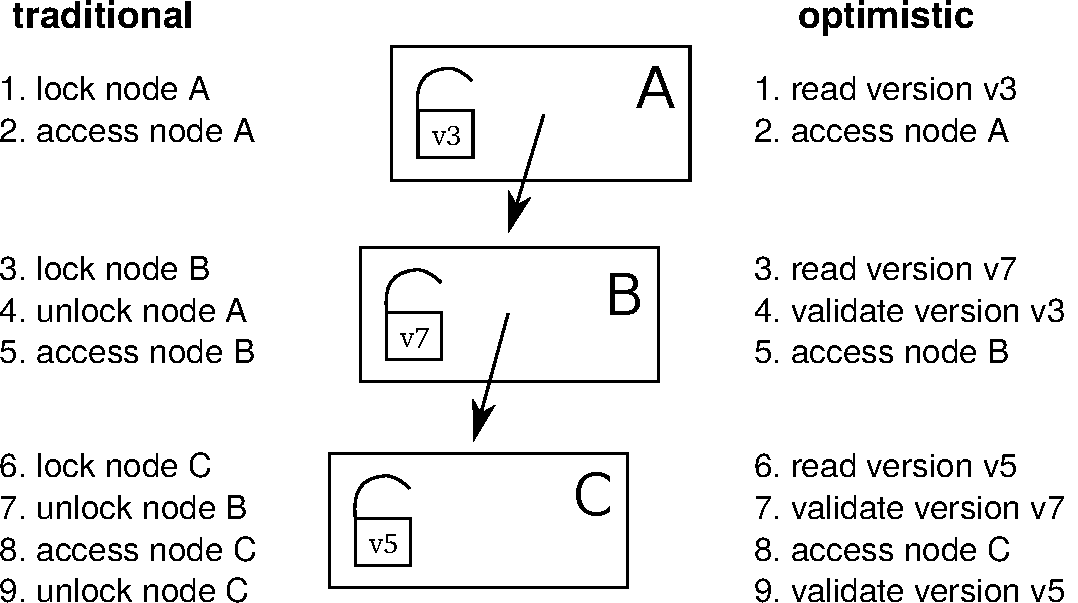
\includegraphics[width=0.65\linewidth]{olcall.pdf}
  \vspace{0.2cm}
  \caption{Comparison of a lookup operation in a 3-level tree using traditional lock coupling (left-hand side) vs.~optimistic lock coupling (right-hand side).}
  \label{fig:olc}
\end{figure}

The traditional and most common lock-based synchronization protocol for B-trees is lock coupling, which interleaves lock acquisitions while holding at most two locks at a time.
If, as we observed earlier, optimistic locks have similar semantics as traditional locks, it is natural to ask whether lock coupling can be combined with optimistic locks.
And indeed the answer is yes: One can almost mechanically translate traditional lock coupling code to optimistic lock coupling code.
This is illustrated in Figure~\ref{fig:olc}, which compares the traversal in a tree of height 3 using traditional and optimistic locks.
As the figure shows, the main difference is that locking is translated to reading the version and that unlocking becomes validation of the previously read version.
This simple change provides efficient lock-free tree traversal without the need to design a complex synchronization protocol.

It is important to emphasize the conceptual simplicity of OLC in comparison to data structures that use custom protocols like the Bw-tree~\cite{DBLP:conf/icde/LevandoskiLS13a}.
To implement lock-free access, the Bw-tree requires an indirection table, delta nodes, complex splitting and merging logic, retry logic, etc.
OLC, on the other hand, can directly be applied to B-trees mostly by adding the appropriate optimistic locking code and without modifying the node layout itself.
Therefore, OpenBw-Tree, an open source implementation of the Bw-tree, requires an order of magnitude more code than a B-tree based on OLC\footnote{Both implementations are available on GitHub: \url{https://github.com/wangziqi2016/index-microbench}}.
Given how difficult it is to develop, validate, and debug lock-free code, simplicity is obviously a major advantage.

\subsection{Correctness Aspects}

\begin{figure}
  % \centering
  %[basicstyle=\normalsize\ttfamily,showstringspaces=false,columns=fullflexible,breaklines=false,breakatwhitespace=true,numbers=none,numberstyle=\small,style=C,keepspaces=true]
\begin{lstlisting}[basicstyle=\ttfamily,language=C++,numbers=left,numberstyle=\small]
std::atomic<BTreeNode*> root;

// search for key in B+tree, returns payload in resultOut
bool lookup(Key key, Value& resultOut) {
   BTreeNode* node = root.load();
   uint64_t nodeVersion = node->readLockOrRestart();
   if (node != root.load()) // make sure the root is still the root
      restart();

   BTreeInner<Key>* parent = nullptr;
   uint64_t parentVersion = 0;

   while (node->isInner()) {
      auto inner = (BTreeInner*)node;

      // unlock parent and make current node the parent
      if (parent)
         parent->readUnlockOrRestart(parentVersion);
      parent = inner;
      parentVersion = nodeVersion;

      // search for next node
      node = inner->findChild(key);
      // validate 'inner' to ensure that 'node' pointer is valid
      inner->checkOrRestart(nodeVersion);
      // now it safe to dereference 'node' pointer (read its version)
      nodeVersion = node->readLockOrRestart();
   }

   // search in leaf and retrieve payload
   auto leaf = (BTreeLeaf*)node;
   bool success = leaf->findValue(key, resultOut);

   // unlock everything
   if (parent)
      parent->readUnlockOrRestart(parentVersion);
   node->readUnlockOrRestart(nodeVersion);

   return success;
}
\end{lstlisting}
  \vspace{0.2cm}
  \caption{B-tree lookup code using OLC. For simplicity, the restart logic is not shown.}
  \label{fig:lookup}
\end{figure}

So far, we have introduced the high-level ideas behind OLC and have stressed its similarity to traditional lock coupling.
Let us now discuss some cases where the close similarity between lock coupling and OLC breaks down.
To make this more concrete, we show the B-tree lookup code in Figure~\ref{fig:lookup}.
In the code, \texttt{readLockOrRestart} reads the lock version and \texttt{readUnlockOrRestart} validates that the read was correct.

One issue with OLC is that any pointer speculatively read from a node may point to invalid memory (if that node is modified concurrently).
Dereferencing such a pointer (e.g., to read its optimistic lock), may cause a segmentation fault or undefined behavior.
In the code shown in Figure~\ref{fig:lookup}, this problem is prevented by the extra check in line 25, which ensures that the read from the node containing the pointer was correct.
Without this additional validation, the code would in line 27 dereference the pointer speculatively read in line 23.
Note that the implementation of \texttt{checkOrRestart} is actually identical to \texttt{readUnlockOrRestart}.
We chose to give it a different name to highlight the fact that this extra check would not be necessary with read/write locks.

Another potential issue with optimistic locks is code that does not terminate.
Code that speculatively accesses a node, like an intra-node binary search, should be written in a way such that it always terminates---even in the presence of concurrent writes.
Otherwise, the validation code that detects the concurrent write will never run.
The binary search of a B-tree, for example, needs to be written in such a way that each comparison makes progress.
For some data structures that do not require loops in the traversal code (like ART) termination is trivially true.

\subsection{Implementation Details}

% implementation, efficiency
To implement an optimistic lock, one can combine the lock and the version counter into a single 64-bit\footnote{Even after subtracting one bit for the lock status, a back-of-the-envelope calculation can show that 63 bits are large enough to never overflow in practice.} word~\cite{artsync}.
A typical read operation will therefore merely consist of reading this version counter atomically.
In C++11 this can be implemented using the \texttt{std::atomic} type.

On x86, atomic reads are cheap because of x86's strong memory order guarantees.
No memory fences are required for sequentially-consistent loads, which are translated (by both GCC and clang) into standard \texttt{MOV} instructions.
Hence, the only effect of \texttt{std::atomic} for loads is preventing instruction re-ordering.
This makes version access and validation cheap.
Acquiring and releasing an optimistic lock in exclusive mode has comparable cost to a traditional lock:
A fairly expensive sequentially-consistent store is needed for acquiring a lock, while a standard \texttt{MOV} suffices for releasing it.
A simple sinlock-based implementation of optimistic locks can be found in the appendix of an earlier paper~\cite{artsync}.

OLC code must be able to handle restarts since validation or lock upgrade can fail due to concurrent writers.
Restarts can easily be implemented by wrapping the data structure operation in a loop (for simplicity not shown in Figure~\ref{fig:lookup}).
Such a loop also enables limiting the number of optimistic retry operations and falling back to pessimistic locking in cases of very heavy contention.
The ability to fall back to traditional locking is a major advantage of OLC in terms of robustness over lock-free approaches, which do not have this option.

In addition to the optimistic shared mode and the exclusive mode, optimistic locks also support a ``shared pessimistic'' mode, which physically acquires the lock in shared mode (allowing multiple concurrent readers but no writers).
This mode is useful for table (or range) scans that touch many tuples on a leaf page (which would otherwise easily abort).
Finally, let us mention that large range scans and table scans, should be broken up into several per-node traversals as is done in the LeanStore~\cite{leanstore} system.

Like all lock-free data structures, but unlike traditional locking and Hardware Transactional Memory~\cite{DBLP:conf/hpca/KarnagelDRLLSL14,DBLP:journals/pvldb/MakreshanskiLS15,htmtkde}, OLC requires care when deleting (and reusing) nodes.
The reason is that a deleting thread can never be sure that a node can be reclaimed because other threads might still be optimistically reading from that node.
Therefore, standard solutions like epoch-based reclamation~\cite{DBLP:conf/sosp/TuZKLM13}, hazard pointers~\cite{DBLP:journals/tpds/Michael04}, or optimized hazard pointers~\cite{DBLP:conf/spaa/BalmauGHZ16} need to be used.
These memory reclamation techniques are, however, largely orthogonal to the synchronization protocol itself.

%-lock-free is not a strong guarantee

\newpage
\section{Evaluation}\label{sec:evaluation}

Let us now experimentally evaluate the overhead and scalability of OLC.
For the experiments, we use an in-memory B+tree implemented in C++11 using templates, which is configured to use nodes of 4096 bytes, random 8 byte keys, and 8 byte payloads.
Based on this B-tree, we compare the following synchronization approaches:
\begin{itemize}
\item an OLC implementation\footnote{An almost identical OLC implementation is available on github: \url{https://github.com/wangziqi2016/index-microbench/tree/master/BTreeOLC}}
\item a variant based on traditional lock coupling and read/write locks
\item the unsynchronized B-tree, which obviously is only correct for read-only workloads but allows measuring the overhead of synchronization
\end{itemize}
Note that earlier work has compared the OLC implementation with a Bw-tree implementation~\cite{buzzword} and other state-of-the-art in-memory index structures.

We use a Haswell EP system with an Intel Xeon E5-2687W v3 CPU, which has 10 cores (20 ``Hyper-Threads'') and 25~MB of L3 cache.
The system is running Ubuntu 18.10 and we use GCC 8.2.0 to compile our code.
The CPU counters are obtained using the Linux perf API\footnote{We use the following convenience wrapper: \url{https://github.com/viktorleis/perfevent}}.

\begin{table}
  \caption{Performance and CPU counters for lookup and insert operations in a B-tree with 100M keys. We perform 100M operations and normalize the CPU counters by that number.}
  \label{tab:overhead}
  \centering
  \begin{tabular}{lrrrrrrr}\toprule
                    &         &        &        & instruc-  & L1     & L3     & branch \\
                    & threads & M op/s & cycles & tions & misses & misses & misses \\\midrule
lookup (no sync.)   & 1       & 1.72   & 2028   & 283     & 39.1   & 14.9   & 16.1   \\
lookup (OLC)        & 1       & 1.65   & 2107   & 370     & 43.9   & 15.1   & 16.7   \\
lookup (lock coup.) & 1       & 1.72   & 2078   & 365     & 42.3   & 16.9   & 15.7   \\\midrule
insert (no sync.)   & 1       & 1.51   & 2286   & 530     & 59.8   & 31.1   & 17.3   \\
insert (OLC)        & 1       & 1.50   & 2303   & 629     & 61.2   & 31.1   & 16.5   \\
insert (lock coup.) & 1       & 1.41   & 2473   & 644     & 61.0   & 31.0   & 17.2   \\\midrule
lookup (no sync.)   & 10      & 15.48  & 2058   & 283     & 38.6   & 15.5   & 16.0   \\
lookup (OLC)        & 10      & 14.60  & 2187   & 370     & 43.8   & 15.8   & 16.8   \\
lookup (lock coup.) & 10      & 5.71   & 5591   & 379     & 54.2   & 17.0   & 14.8   \\\midrule
insert (no sync.)   & 10      & -      & -      & -       & -      & -      & -      \\
insert (OLC)        & 10      & 10.46  & 2940   & 656     & 62.0   & 32.5   & 16.8   \\
insert (lock coup.) & 10      & 7.55   & 4161   & 667     & 75.0   & 28.6   & 16.2   \\
    \bottomrule
\end{tabular}
\end{table}

Table~\ref{tab:overhead} compares the performance and CPU counters for lookup and insert operations in a B-tree with 100M keys.
With {\em single-threaded} execution, we observe that all three approaches have very similar performance.
Adding traditional or optimistic locks to unsynchronized B-tree code results in up to 30\% of additional instructions without affecting single-threaded performance much.

\begin{figure}
  \centering
  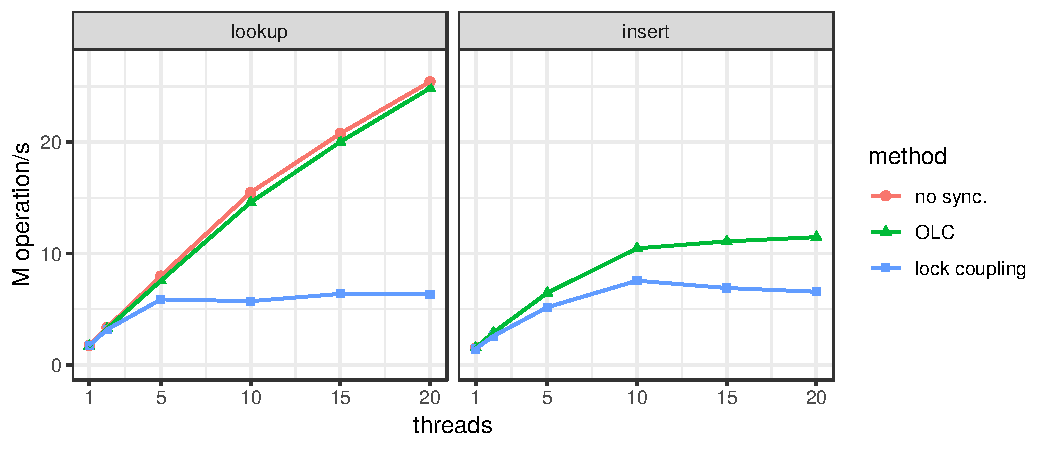
\includegraphics[width=\linewidth]{scale.pdf}
  \vspace{0.2cm}
  \caption{Scalability on 10-core system for B-tree operations (100M values).}
  \label{fig:scale}
\end{figure}

As Figure~\ref{fig:scale} shows, the results change dramatically once we use multiple threads.
For lookup, the scalability of OLC is near-linear up to 20 threads, even though the system has only 10 ``real cores''.
The OLC scalability for insert is also respectable (though not quite as linear because multi-threaded insertion approaches the memory bandwidth of our processor).
The figure also shows that the results of traditional lock coupling with read/write locks are significantly worse than OLC.
With 20 threads, lookup with OLC is 3.9$\times$ faster than traditional lock coupling.

\section{Summary}\label{sec:conc}

Optimistic Lock Coupling (OLC) is an effective synchronization method that combines the simplicity of traditional lock coupling with the superior scalability of lock-free approaches.
OLC is widely applicable and has already been successfully used to synchronize several data structures, including B-trees, binary search trees, and different trie variants.
These features make it highly attractive for modern database systems as well as performance-critical systems software in general.

\begin{thebibliography}{10}

\bibitem{DBLP:conf/spaa/BalmauGHZ16}
O.~Balmau, R.~Guerraoui, M.~Herlihy, and I.~Zablotchi.
\newblock Fast and robust memory reclamation for concurrent data structures.
\newblock In {\em SPAA}, 2016.

\bibitem{DBLP:journals/acta/BayerS77}
R.~Bayer and M.~Schkolnick.
\newblock Concurrency of operations on {B}-trees.
\newblock {\em Acta Informatica}, 9, 1977.

\bibitem{hot}
R.~Binna, E.~Zangerle, M.~Pichl, G.~Specht, and V.~Leis.
\newblock {HOT}: A height optimized trie index for main-memory database
  systems.
\newblock In {\em SIGMOD}, 2018.

\bibitem{DBLP:conf/ppopp/BronsonCCO10}
N.~G. Bronson, J.~Casper, H.~Chafi, and K.~Olukotun.
\newblock A practical concurrent binary search tree.
\newblock In {\em PPOPP}, 2010.

\bibitem{DBLP:conf/vldb/ChaHKK01}
S.~K. Cha, S.~Hwang, K.~Kim, and K.~Kwon.
\newblock Cache-conscious concurrency control of main-memory indexes on
  shared-memory multiprocessor systems.
\newblock In {\em VLDB}, 2001.

\bibitem{intel}
I.~Cutress.
\newblock {Intel} goes for 48-cores: {Cascade-AP} with multi-chip package
  coming soon.
\newblock
  \url{https://www.anandtech.com/show/13535/intel-goes-for-48cores-cascade-ap},
  2018 (accessed January, 2019).

\bibitem{DBLP:conf/cidr/FaleiroA17}
J.~M. Faleiro and D.~J. Abadi.
\newblock Latch-free synchronization in database systems: Silver bullet or
  fool's gold?
\newblock In {\em CIDR}, 2017.

\bibitem{DBLP:journals/ftdb/Graefe11}
G.~Graefe.
\newblock Modern {B}-tree techniques.
\newblock {\em Foundations and Trends in Databases}, 3(4), 2011.

\bibitem{DBLP:conf/hpca/KarnagelDRLLSL14}
T.~Karnagel, R.~Dementiev, R.~Rajwar, K.~Lai, T.~Legler, B.~Schlegel, and
  W.~Lehner.
\newblock Improving in-memory database index performance with
  {Intel}\({}^{\mbox{{\textregistered}}}\) transactional synchronization
  extensions.
\newblock In {\em HPCA}, 2014.

\bibitem{DBLP:journals/tods/LehmanY81}
P.~L. Lehman and S.~B. Yao.
\newblock Efficient locking for concurrent operations on {B}-trees.
\newblock {\em {ACM} Trans. Database Syst.}, 6(4), 1981.

\bibitem{leanstore}
V.~Leis, M.~Haubenschild, A.~Kemper, and T.~Neumann.
\newblock Leanstore: In-memory data management beyond main memory.
\newblock In {\em ICDE}, 2018.

\bibitem{art}
V.~Leis, A.~Kemper, and T.~Neumann.
\newblock The adaptive radix tree: {ARTful} indexing for main-memory databases.
\newblock In {\em ICDE}, 2013.

\bibitem{htmtkde}
V.~Leis, A.~Kemper, and T.~Neumann.
\newblock Scaling {HTM}-supported database transactions to many cores.
\newblock {\em {IEEE} Trans. Knowl. Data Eng.}, 28(2), 2016.

\bibitem{artsync}
V.~Leis, F.~Scheibner, A.~Kemper, and T.~Neumann.
\newblock The {ART} of practical synchronization.
\newblock In {\em DaMoN}, 2016.

\bibitem{DBLP:conf/icde/LevandoskiLS13a}
J.~J. Levandoski, D.~B. Lomet, and S.~Sengupta.
\newblock The {Bw}-tree: A {B}-tree for new hardware platforms.
\newblock In {\em ICDE}, 2013.

\bibitem{DBLP:journals/pvldb/MakreshanskiLS15}
D.~Makreshanski, J.~J. Levandoski, and R.~Stutsman.
\newblock To lock, swap, or elide: On the interplay of hardware transactional
  memory and lock-free indexing.
\newblock {\em {PVLDB}}, 8(11), 2015.

\bibitem{DBLP:dblp_conf/eurosys/MaoKM12}
Y.~Mao, E.~Kohler, and R.~T. Morris.
\newblock Cache craftiness for fast multicore key-value storage.
\newblock In {\em EuroSys}, 2012.

\bibitem{DBLP:journals/tpds/Michael04}
M.~M. Michael.
\newblock Hazard pointers: Safe memory reclamation for lock-free objects.
\newblock {\em {IEEE} Trans. Parallel Distrib. Syst.}, 15(6), 2004.

\bibitem{DBLP:journals/jacm/ShalevS06}
O.~Shalev and N.~Shavit.
\newblock Split-ordered lists: Lock-free extensible hash tables.
\newblock {\em J. {ACM}}, 53(3), 2006.

\bibitem{amd}
A.~Shilov.
\newblock {AMD} previews {EPYC} ‘{Rome}’ processor: Up to 64 {Zen} 2 cores.
\newblock
  \url{https://www.anandtech.com/show/13561/amd-previews-epyc-rome-processor-up-to-64-zen-2-cores},
  2018 (accessed January, 2019).

\bibitem{DBLP:conf/sosp/TuZKLM13}
S.~Tu, W.~Zheng, E.~Kohler, B.~Liskov, and S.~Madden.
\newblock Speedy transactions in multicore in-memory databases.
\newblock In {\em SOSP}, 2013.

\bibitem{buzzword}
Z.~Wang, A.~Pavlo, H.~Lim, V.~Leis, H.~Zhang, M.~Kaminsky, and D.~Andersen.
\newblock Building a {Bw}-tree takes more than just buzz words.
\newblock In {\em SIGMOD}, 2018.

\end{thebibliography}


%\bibliographystyle{abbrv}
%\bibliography{main}

\end{document}

\end{article}

\begin{article}
{Navigating Compliance with Data Transfers in Federated Data Processing}
{Kaustubh Beedkar, Jorge Quian\'e, Volker Markl}
\graphicspath{{submissions/navigating-compliance-with-data-transfers-in-federated-data-processing/}}
\pdfminorversion=5
\documentclass[11pt]{article}
\usepackage{deauthor,times,graphicx,caption,microtype}
\usepackage{hyperref}
\usepackage{listings}
\usepackage{booktabs}

\begin{document}

\title{Optimistic Lock Coupling: A Scalable and Efficient General-Purpose Synchronization Method}

\author{Viktor Leis, Michael Haubenschild\raisebox{0.9ex}{$\ast$}, Thomas Neumann\\ Technische Universit{\"a}t M{\"u}nchen \hspace{0.7cm} Tableau Software\raisebox{0.9ex}{$\ast$} \\ {\{leis,neumann\}{@}in.tum.de} \hspace{0.7cm} {mhaubenschild{@}tableau.com\raisebox{0.9ex}{$\ast$}}}

\maketitle

\begin{abstract}
As the number of cores on commodity processors continues to increase, scalability becomes more and more crucial for overall performance.
Scalable and efficient concurrent data structures are particularly important, as these are often the building blocks of parallel algorithms.
Unfortunately, traditional synchronization techniques based on fine-grained locking have been shown to be unscalable on modern multi-core CPUs.
Lock-free data structures, on the other hand, are extremely difficult to design and often incur significant overhead.

In this work, we make the case for Optimistic Lock Coupling as a practical alternative to both traditional locking and the lock-free approach.
We show that Optimistic Lock Coupling is highly scalable and almost as simple to implement as traditional lock coupling.
Another important advantage is that it is easily applicable to most tree-like data structures.
We therefore argue that Optimistic Lock Coupling, rather than a complex and error-prone custom synchronization protocol, should be the default choice for performance-critical data structures.
\end{abstract}

\section{Introduction}

% more and more cores
Today, Intel's commodity server processors have up to 28 cores and its upcoming microarchitecture will have up to 48 cores per socket~\cite{intel}.
Similarly, AMD currently stands at 32 cores and this number is expected to double in the next generation~\cite{amd}.
Since both platforms support simultaneous multithreading (also known as hyperthreading), affordable commodity servers (with up to two sockets) will soon routinely have between 100 and 200 hardware threads.

% data structure scalability is important
With such a high degree of hardware parallelism, efficient data processing crucially depends on how well concurrent data structures scale.
Internally, database systems use a plethora of data structures like table heaps, internal work queues, and, most importantly, index structures.
Any of these can easily become a scalability (and therefore overall performance) bottleneck on many-core CPUs.

% traditional synchronization: fine-grained locks, slow, cache invalidation
Traditionally, database systems synchronize internal data structures using fine-grained reader/writer locks\footnote{In this work, we focus on data structure synchronization rather than high-level transaction semantics and therefore use the term {\em lock} for what would typically be called {\em latch} in the database literature. We thus follow common computer science (rather than database) terminology.}.
Unfortunately, while fine-grained locking makes lock contention unlikely, it still results in bad scalability because lock acquisition and release require writing to shared memory.
Due to the way cache coherency is implemented on modern multi-core CPUs, these writes cause additional cache misses\footnote{The cache coherency protocol ensures that all copies of a cache line on other cores are invalidated before the write can proceed.} and the cache line containing the lock's internal data becomes a point of physical contention.
As a result, any frequently-accessed lock (e.g., the lock of the root node of a B-tree) severely limits scalability.

% lock-free bw-tree: no more latches, but indirections, extremely complex
Lock-free data structures like the Bw-tree~\cite{DBLP:conf/icde/LevandoskiLS13a} (a lock-free B-tree variant) or the Split-Ordered List~\cite{DBLP:journals/jacm/ShalevS06} (a lock-free hash table) do not acquire any locks and therefore generally scale much better than locking-based approaches (in particular for read-mostly workloads).
However, lock-free synchronization has other downsides:
First, it is very difficult and results in extremely complex and error-prone code (when compared to locking).
Second, because the functionality of atomic primitives provided by the hardware (e.g., atomically compare-and-swap 8 bytes) is limited, complex operations require additional indirections within the data structure.
For example, the Bw-tree requires an indirection table and the Split-Ordered List requires ``dummy nodes'', resulting in overhead due to additional cache misses.

% OLC for the win
In this paper we make the case for {\em Optimistic Lock Coupling (OLC)}, a synchronization method that combines some of the best properties of lock-based and lock-free synchronization.
OLC utilizes a special lock type that can be used in two modes:
The first mode is similar to a traditional mutex and excludes other threads by physically acquiring the underlying lock.
In the second mode, reads can proceed optimistically by validating a version counter that is embedded in the lock (similar to optimistic concurrency control).
The first mode is typically used by writers and the second mode by readers.
Besides this special lock type, OLC is based on the observation that optimistic lock validations can be interleaved/coupled---similar to the pair-wise interleaved lock acquisition of traditional lock coupling.
Hence, the name Optimistic Lock Coupling.

OLC has a number of desirable features:
\begin{itemize}
\item By reducing the number of writes to shared memory locations and thereby avoiding cache invalidations, it {\bf scales well} for most workloads.
\item In comparison to unsynchronized code, it requires few additional CPU instructions making it {\bf efficient}.
\item OLC is {\bf widely applicable} to different data structures. It has already been successfully used for synchronizing binary search trees~\cite{DBLP:conf/ppopp/BronsonCCO10}, tries~\cite{artsync}, trie/B-tree hybrids~\cite{DBLP:dblp_conf/eurosys/MaoKM12}, and B-trees~\cite{buzzword}.
\item In comparison to the lock-free paradigm, it is also {\bf easy to use} and requires few modifications to existing, single-threaded data structures.
\end{itemize}
Despite these positive features and its simplicity, OLC is not yet widely known.
The goal of this paper is therefore to popularize this simple idea and to make a case for it.
We argue that OLC deserves to be widely known.
It is a good default synchronization paradigm---more complex, data structure-specific protocols are seldom beneficial.

The rest of the paper is organized as follows.
Section~\ref{sec:related} discusses related work, tracing the history of OLC and its underlying ideas in the literature.
The core of the paper is Section~\ref{sec:olc}, which describes the ideas behind OLC and how it can be used to synchronize complex data structures.
In Section~\ref{sec:evaluation} we experimentally show that OLC has low overhead and scales well when used to synchronize an in-memory B-tree.
We summarize the paper in Section~\ref{sec:conc}.

\newpage
\section{Related Work}\label{sec:related}

Lock coupling has been proposed as a method for allowing concurrent operations on B-trees in 1977~\cite{DBLP:journals/acta/BayerS77}.
This traditional and still widely-used method, described in detail in Graefe's B-tree survey~\cite{DBLP:journals/ftdb/Graefe11}, is also called ``latch coupling'', ``hand-over-hand locking'', and ``crabbing''.
Because at most two locks are held at-a-time during tree traversal, this technique seemingly allows for a high degree of parallelism---in particular if read/write locks are used to enable inner nodes to be locked in shared mode.
However, as we show in Section~\ref{sec:evaluation}, on modern hardware lock acquisition (even in shared mode) results in suboptimal scalability.

An early alternative from 1981 is a B-tree variant called B-link tree~\cite{DBLP:journals/tods/LehmanY81}, which only holds a single lock at a time.
It is based on the observation that between the release of the parent lock and the acquisition of the child lock, the only ``dangerous'' thing that could have happened is the split of a child node (assuming one does not implement merge operations).
Thus, when a split happens, the key being searched might end up on a neighboring node to the right of the current child node.
A B-link tree traversal therefore detects this condition and, if needed, transparently proceeds to the neighboring node.
Releasing the parent lock early is highly beneficial when the child node needs to be fetched from disk.
For in-memory workloads, however, the B-link tree has the same scalability issues as lock coupling (it acquires just as many locks).

The next major advance, Optimistic Latch-Free Index Traversal (OLFIT)~\cite{DBLP:conf/vldb/ChaHKK01}, was proposed in 2001.
OLFIT introduced the idea of a combined lock/update counter, which we call {\em optimistic lock}. % , for lack of a better name,
Based on these per-node optimistic locks and the synchronization protocol of the B-link tree, OLFIT finally achieves good scalability on parallel processors.
The OLFIT protocol is fairly complex, as it requires both the non-trivial B-link protocol and optimistic locks.
Furthermore, like the B-link tree protocol, it does not support merging nodes, and is specific to B-trees (cannot easily be applied to other data structures).

In the following two decades, the growth of main-memory capacity led to much research into other data structures besides the venerable B-tree.
Particularly relevant for our discussion is Bronson et al.'s~\cite{DBLP:conf/ppopp/BronsonCCO10} concurrent binary search tree, which is based on optimistic version validation and has a sophisticated, data structure-specific synchronization protocol.
To the best of our knowledge, this 2010 paper is the first that, as part of its protocol, interleaves version validation across nodes---rather than validating each node separately like OLFIT.
In that paper, this idea is called ``hand-over-hand, optimistic validation'', while we prefer the term Optimistic Lock Coupling to highlight the close resemblance to traditional lock coupling.
Similarly, Mao et al.'s~\cite{DBLP:dblp_conf/eurosys/MaoKM12} Masstree (a concurrent hybrid trie/B-tree) is also based on the same ideas, but again uses them as part of a more complex protocol.

The Adaptive Radix Tree (ART)~\cite{art} is another recent in-memory data structure, which we proposed in 2013.
In contrast to the two data structures just mentioned, it was originally designed with single-threaded performance in mind without supporting concurrency.
To add support for concurrency, we initially started designing a custom protocol called Read-Optimized Write Exclusion (ROWEX)~\cite{artsync}, which turned out to be non-trivial and requires modifications of the underlying data structure\footnote{Note that ROWEX is already easier to apply to existing data structures than the lock-free approach. The difficulty depends on the data structure. Applying ROWEX is hard for B-trees with sorted keys and fairly easy for copy-on-write data structures like the Height Optimized Trie~\cite{hot}---with ART being somewhere in the middle.}.
However, fairly late in the project, we also realized, that OLC {\em alone} (rather than as part of a more complex protocol) is sufficient to synchronize ART.
No other changes to the data structure were necessary.
Both approaches were published and experimentally evaluated in a followup paper~\cite{artsync}, which shows that, despite its simplicity, OLC is efficient, scalable, and generally outperforms ROWEX.

Similar results were recently published regarding B-trees~\cite{buzzword}.
In this experimental study a simple OLC-based synchronization outperformed the Bw-tree~\cite{DBLP:conf/icde/LevandoskiLS13a}, a complex lock-free synchronization approach.
Another recent paper shows that for write-intensive workloads, locking often performs better than lock-free synchronization~\cite{DBLP:conf/cidr/FaleiroA17}.
These experiences indicate that OLC is a general-purpose synchronization paradigm and motivate the current paper.

%foster b-tree\cite{DBLP:journals/tods/GraefeKK12}
%Shasha theory~\cite{DBLP:journals/tods/ShashaG88}

\section{Optimistic Lock Coupling}\label{sec:olc}

% locks suck
The standard technique for inter-thread synchronization is mutual exclusion using fine-grained locks.
In a B-tree, for example, every node usually has its own associated lock, which is acquired before accessing that node.
The problem of locking on modern multi- and many-core processors is that lock acquisition and release require writing to the shared memory location that implements the lock.
This write causes exclusive ownership of the underlying cache line and invalidates copies of it on all other processor cores.
For hierarchical, tree-like data structures, the lock of the root node becomes a point of physical contention---even in read-only workloads and even when read/write locks are used.
Depending on the specific data structure, number of cores, cache coherency protocol implementation, cache topology, whether Non-Uniform Memory Access (NUMA) is used, locking can even result in multi-threaded performance that is worse than single-threaded execution.

% in b-trees this happens very much
The inherent pessimism of locking is particularly unfortunate for B-trees:
Despite the fact that logical modifications of the root node are very infrequent, every B-tree operation must lock the root node during tree traversal\footnote{To a lesser extent this obviously applies to all inner nodes, not just the root.}.
Even the vast majority of update operations (with the exception of splits and merges), only modify a single leaf node.
These observations indicate that a more optimistic approach, which does not require locking inner nodes, would be very beneficial for B-trees.

\subsection{Optimistic Locks}

% optimism to the rescue
As the name indicates, optimistic locks try to solve the scalability issues of traditional locks using an optimistic approach.
Instead of always physically acquiring locks, even for nodes that are unlikely to be modified simultaneously, after-the-fact validation is used to detect conflicts.
This is done by augmenting each lock with a version/update counter that is incremented on every modification.
Using this version counter, readers can optimistically proceed before validating that the version did not change to ensure that the read was safe.
If validation fails, the operation is restarted.

% details on opt locks
Using optimistic locks, a read-only node access (i.e., the majority of all operations in a B-tree) does not acquire the lock and does not increment the version counter.
Instead, it performs the following steps:
\begin{enumerate}
\item read lock version (restart if lock is not free)
\item access node
\item read the version again and validate that it has not changed in the meantime
\end{enumerate}
If the last step (the validation) fails, the operation has to be restarted.
Write operations, on the other hand, are more similar to traditional locking:
\begin{enumerate}
\item acquire lock (wait if necessary)
\item access/write to node
\item increment version and unlock node
\end{enumerate}
Writes can therefore protect a node from other writes.

% similar to locks
As we observed in an earlier paper~\cite{artsync}, because of similar semantics, optimistic locks can be hidden behind an API very similar to traditional read/write locks.
Both approaches have an exclusive lock mode, and acquiring a traditional lock in shared mode is analogous to optimistic version validation.
Furthermore, like with some implementations of traditional read/write locks, optimistic locks allow upgrading a shared lock to an exclusive lock.
Lock upgrades are, for example, used to avoid most B-tree update operations from having to lock inner nodes.
In our experience, the close resemblance of optimistic and traditional locks simplifies the reasoning about optimistic locks;
one can apply similar thinking as in traditional lock-based protocols.

\subsection{Lock Coupling with Optimistic Locks}

\begin{figure}
  \centering
  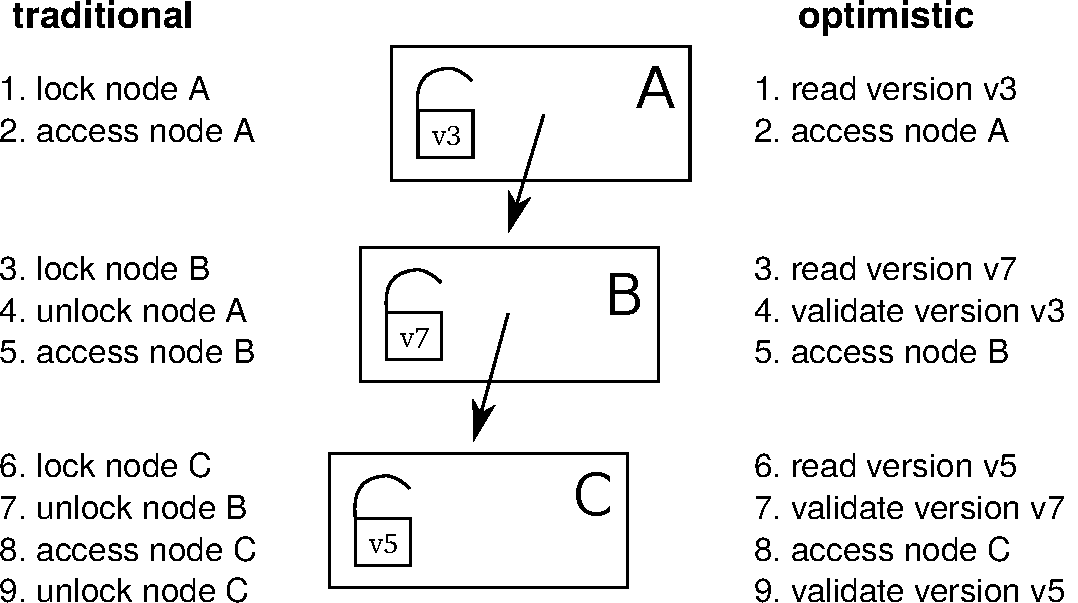
\includegraphics[width=0.65\linewidth]{olcall.pdf}
  \vspace{0.2cm}
  \caption{Comparison of a lookup operation in a 3-level tree using traditional lock coupling (left-hand side) vs.~optimistic lock coupling (right-hand side).}
  \label{fig:olc}
\end{figure}

The traditional and most common lock-based synchronization protocol for B-trees is lock coupling, which interleaves lock acquisitions while holding at most two locks at a time.
If, as we observed earlier, optimistic locks have similar semantics as traditional locks, it is natural to ask whether lock coupling can be combined with optimistic locks.
And indeed the answer is yes: One can almost mechanically translate traditional lock coupling code to optimistic lock coupling code.
This is illustrated in Figure~\ref{fig:olc}, which compares the traversal in a tree of height 3 using traditional and optimistic locks.
As the figure shows, the main difference is that locking is translated to reading the version and that unlocking becomes validation of the previously read version.
This simple change provides efficient lock-free tree traversal without the need to design a complex synchronization protocol.

It is important to emphasize the conceptual simplicity of OLC in comparison to data structures that use custom protocols like the Bw-tree~\cite{DBLP:conf/icde/LevandoskiLS13a}.
To implement lock-free access, the Bw-tree requires an indirection table, delta nodes, complex splitting and merging logic, retry logic, etc.
OLC, on the other hand, can directly be applied to B-trees mostly by adding the appropriate optimistic locking code and without modifying the node layout itself.
Therefore, OpenBw-Tree, an open source implementation of the Bw-tree, requires an order of magnitude more code than a B-tree based on OLC\footnote{Both implementations are available on GitHub: \url{https://github.com/wangziqi2016/index-microbench}}.
Given how difficult it is to develop, validate, and debug lock-free code, simplicity is obviously a major advantage.

\subsection{Correctness Aspects}

\begin{figure}
  % \centering
  %[basicstyle=\normalsize\ttfamily,showstringspaces=false,columns=fullflexible,breaklines=false,breakatwhitespace=true,numbers=none,numberstyle=\small,style=C,keepspaces=true]
\begin{lstlisting}[basicstyle=\ttfamily,language=C++,numbers=left,numberstyle=\small]
std::atomic<BTreeNode*> root;

// search for key in B+tree, returns payload in resultOut
bool lookup(Key key, Value& resultOut) {
   BTreeNode* node = root.load();
   uint64_t nodeVersion = node->readLockOrRestart();
   if (node != root.load()) // make sure the root is still the root
      restart();

   BTreeInner<Key>* parent = nullptr;
   uint64_t parentVersion = 0;

   while (node->isInner()) {
      auto inner = (BTreeInner*)node;

      // unlock parent and make current node the parent
      if (parent)
         parent->readUnlockOrRestart(parentVersion);
      parent = inner;
      parentVersion = nodeVersion;

      // search for next node
      node = inner->findChild(key);
      // validate 'inner' to ensure that 'node' pointer is valid
      inner->checkOrRestart(nodeVersion);
      // now it safe to dereference 'node' pointer (read its version)
      nodeVersion = node->readLockOrRestart();
   }

   // search in leaf and retrieve payload
   auto leaf = (BTreeLeaf*)node;
   bool success = leaf->findValue(key, resultOut);

   // unlock everything
   if (parent)
      parent->readUnlockOrRestart(parentVersion);
   node->readUnlockOrRestart(nodeVersion);

   return success;
}
\end{lstlisting}
  \vspace{0.2cm}
  \caption{B-tree lookup code using OLC. For simplicity, the restart logic is not shown.}
  \label{fig:lookup}
\end{figure}

So far, we have introduced the high-level ideas behind OLC and have stressed its similarity to traditional lock coupling.
Let us now discuss some cases where the close similarity between lock coupling and OLC breaks down.
To make this more concrete, we show the B-tree lookup code in Figure~\ref{fig:lookup}.
In the code, \texttt{readLockOrRestart} reads the lock version and \texttt{readUnlockOrRestart} validates that the read was correct.

One issue with OLC is that any pointer speculatively read from a node may point to invalid memory (if that node is modified concurrently).
Dereferencing such a pointer (e.g., to read its optimistic lock), may cause a segmentation fault or undefined behavior.
In the code shown in Figure~\ref{fig:lookup}, this problem is prevented by the extra check in line 25, which ensures that the read from the node containing the pointer was correct.
Without this additional validation, the code would in line 27 dereference the pointer speculatively read in line 23.
Note that the implementation of \texttt{checkOrRestart} is actually identical to \texttt{readUnlockOrRestart}.
We chose to give it a different name to highlight the fact that this extra check would not be necessary with read/write locks.

Another potential issue with optimistic locks is code that does not terminate.
Code that speculatively accesses a node, like an intra-node binary search, should be written in a way such that it always terminates---even in the presence of concurrent writes.
Otherwise, the validation code that detects the concurrent write will never run.
The binary search of a B-tree, for example, needs to be written in such a way that each comparison makes progress.
For some data structures that do not require loops in the traversal code (like ART) termination is trivially true.

\subsection{Implementation Details}

% implementation, efficiency
To implement an optimistic lock, one can combine the lock and the version counter into a single 64-bit\footnote{Even after subtracting one bit for the lock status, a back-of-the-envelope calculation can show that 63 bits are large enough to never overflow in practice.} word~\cite{artsync}.
A typical read operation will therefore merely consist of reading this version counter atomically.
In C++11 this can be implemented using the \texttt{std::atomic} type.

On x86, atomic reads are cheap because of x86's strong memory order guarantees.
No memory fences are required for sequentially-consistent loads, which are translated (by both GCC and clang) into standard \texttt{MOV} instructions.
Hence, the only effect of \texttt{std::atomic} for loads is preventing instruction re-ordering.
This makes version access and validation cheap.
Acquiring and releasing an optimistic lock in exclusive mode has comparable cost to a traditional lock:
A fairly expensive sequentially-consistent store is needed for acquiring a lock, while a standard \texttt{MOV} suffices for releasing it.
A simple sinlock-based implementation of optimistic locks can be found in the appendix of an earlier paper~\cite{artsync}.

OLC code must be able to handle restarts since validation or lock upgrade can fail due to concurrent writers.
Restarts can easily be implemented by wrapping the data structure operation in a loop (for simplicity not shown in Figure~\ref{fig:lookup}).
Such a loop also enables limiting the number of optimistic retry operations and falling back to pessimistic locking in cases of very heavy contention.
The ability to fall back to traditional locking is a major advantage of OLC in terms of robustness over lock-free approaches, which do not have this option.

In addition to the optimistic shared mode and the exclusive mode, optimistic locks also support a ``shared pessimistic'' mode, which physically acquires the lock in shared mode (allowing multiple concurrent readers but no writers).
This mode is useful for table (or range) scans that touch many tuples on a leaf page (which would otherwise easily abort).
Finally, let us mention that large range scans and table scans, should be broken up into several per-node traversals as is done in the LeanStore~\cite{leanstore} system.

Like all lock-free data structures, but unlike traditional locking and Hardware Transactional Memory~\cite{DBLP:conf/hpca/KarnagelDRLLSL14,DBLP:journals/pvldb/MakreshanskiLS15,htmtkde}, OLC requires care when deleting (and reusing) nodes.
The reason is that a deleting thread can never be sure that a node can be reclaimed because other threads might still be optimistically reading from that node.
Therefore, standard solutions like epoch-based reclamation~\cite{DBLP:conf/sosp/TuZKLM13}, hazard pointers~\cite{DBLP:journals/tpds/Michael04}, or optimized hazard pointers~\cite{DBLP:conf/spaa/BalmauGHZ16} need to be used.
These memory reclamation techniques are, however, largely orthogonal to the synchronization protocol itself.

%-lock-free is not a strong guarantee

\newpage
\section{Evaluation}\label{sec:evaluation}

Let us now experimentally evaluate the overhead and scalability of OLC.
For the experiments, we use an in-memory B+tree implemented in C++11 using templates, which is configured to use nodes of 4096 bytes, random 8 byte keys, and 8 byte payloads.
Based on this B-tree, we compare the following synchronization approaches:
\begin{itemize}
\item an OLC implementation\footnote{An almost identical OLC implementation is available on github: \url{https://github.com/wangziqi2016/index-microbench/tree/master/BTreeOLC}}
\item a variant based on traditional lock coupling and read/write locks
\item the unsynchronized B-tree, which obviously is only correct for read-only workloads but allows measuring the overhead of synchronization
\end{itemize}
Note that earlier work has compared the OLC implementation with a Bw-tree implementation~\cite{buzzword} and other state-of-the-art in-memory index structures.

We use a Haswell EP system with an Intel Xeon E5-2687W v3 CPU, which has 10 cores (20 ``Hyper-Threads'') and 25~MB of L3 cache.
The system is running Ubuntu 18.10 and we use GCC 8.2.0 to compile our code.
The CPU counters are obtained using the Linux perf API\footnote{We use the following convenience wrapper: \url{https://github.com/viktorleis/perfevent}}.

\begin{table}
  \caption{Performance and CPU counters for lookup and insert operations in a B-tree with 100M keys. We perform 100M operations and normalize the CPU counters by that number.}
  \label{tab:overhead}
  \centering
  \begin{tabular}{lrrrrrrr}\toprule
                    &         &        &        & instruc-  & L1     & L3     & branch \\
                    & threads & M op/s & cycles & tions & misses & misses & misses \\\midrule
lookup (no sync.)   & 1       & 1.72   & 2028   & 283     & 39.1   & 14.9   & 16.1   \\
lookup (OLC)        & 1       & 1.65   & 2107   & 370     & 43.9   & 15.1   & 16.7   \\
lookup (lock coup.) & 1       & 1.72   & 2078   & 365     & 42.3   & 16.9   & 15.7   \\\midrule
insert (no sync.)   & 1       & 1.51   & 2286   & 530     & 59.8   & 31.1   & 17.3   \\
insert (OLC)        & 1       & 1.50   & 2303   & 629     & 61.2   & 31.1   & 16.5   \\
insert (lock coup.) & 1       & 1.41   & 2473   & 644     & 61.0   & 31.0   & 17.2   \\\midrule
lookup (no sync.)   & 10      & 15.48  & 2058   & 283     & 38.6   & 15.5   & 16.0   \\
lookup (OLC)        & 10      & 14.60  & 2187   & 370     & 43.8   & 15.8   & 16.8   \\
lookup (lock coup.) & 10      & 5.71   & 5591   & 379     & 54.2   & 17.0   & 14.8   \\\midrule
insert (no sync.)   & 10      & -      & -      & -       & -      & -      & -      \\
insert (OLC)        & 10      & 10.46  & 2940   & 656     & 62.0   & 32.5   & 16.8   \\
insert (lock coup.) & 10      & 7.55   & 4161   & 667     & 75.0   & 28.6   & 16.2   \\
    \bottomrule
\end{tabular}
\end{table}

Table~\ref{tab:overhead} compares the performance and CPU counters for lookup and insert operations in a B-tree with 100M keys.
With {\em single-threaded} execution, we observe that all three approaches have very similar performance.
Adding traditional or optimistic locks to unsynchronized B-tree code results in up to 30\% of additional instructions without affecting single-threaded performance much.

\begin{figure}
  \centering
  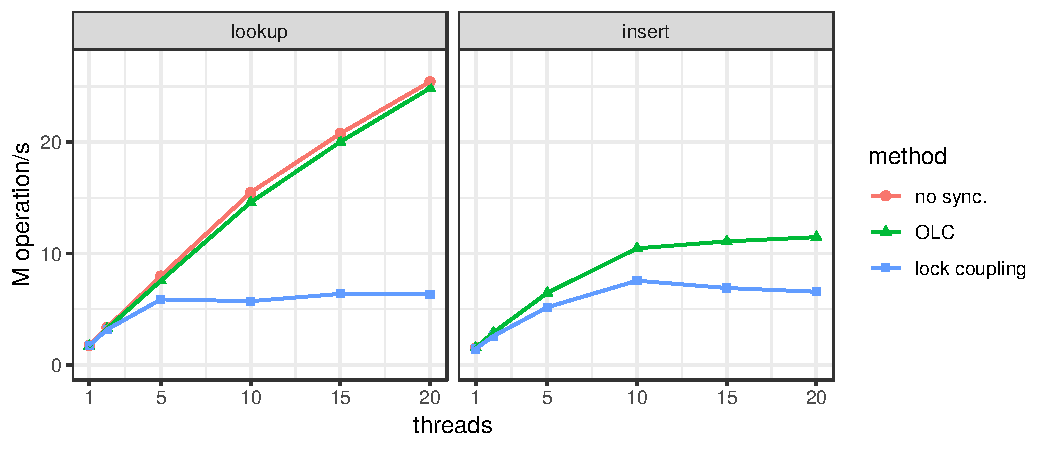
\includegraphics[width=\linewidth]{scale.pdf}
  \vspace{0.2cm}
  \caption{Scalability on 10-core system for B-tree operations (100M values).}
  \label{fig:scale}
\end{figure}

As Figure~\ref{fig:scale} shows, the results change dramatically once we use multiple threads.
For lookup, the scalability of OLC is near-linear up to 20 threads, even though the system has only 10 ``real cores''.
The OLC scalability for insert is also respectable (though not quite as linear because multi-threaded insertion approaches the memory bandwidth of our processor).
The figure also shows that the results of traditional lock coupling with read/write locks are significantly worse than OLC.
With 20 threads, lookup with OLC is 3.9$\times$ faster than traditional lock coupling.

\section{Summary}\label{sec:conc}

Optimistic Lock Coupling (OLC) is an effective synchronization method that combines the simplicity of traditional lock coupling with the superior scalability of lock-free approaches.
OLC is widely applicable and has already been successfully used to synchronize several data structures, including B-trees, binary search trees, and different trie variants.
These features make it highly attractive for modern database systems as well as performance-critical systems software in general.

\begin{thebibliography}{10}

\bibitem{DBLP:conf/spaa/BalmauGHZ16}
O.~Balmau, R.~Guerraoui, M.~Herlihy, and I.~Zablotchi.
\newblock Fast and robust memory reclamation for concurrent data structures.
\newblock In {\em SPAA}, 2016.

\bibitem{DBLP:journals/acta/BayerS77}
R.~Bayer and M.~Schkolnick.
\newblock Concurrency of operations on {B}-trees.
\newblock {\em Acta Informatica}, 9, 1977.

\bibitem{hot}
R.~Binna, E.~Zangerle, M.~Pichl, G.~Specht, and V.~Leis.
\newblock {HOT}: A height optimized trie index for main-memory database
  systems.
\newblock In {\em SIGMOD}, 2018.

\bibitem{DBLP:conf/ppopp/BronsonCCO10}
N.~G. Bronson, J.~Casper, H.~Chafi, and K.~Olukotun.
\newblock A practical concurrent binary search tree.
\newblock In {\em PPOPP}, 2010.

\bibitem{DBLP:conf/vldb/ChaHKK01}
S.~K. Cha, S.~Hwang, K.~Kim, and K.~Kwon.
\newblock Cache-conscious concurrency control of main-memory indexes on
  shared-memory multiprocessor systems.
\newblock In {\em VLDB}, 2001.

\bibitem{intel}
I.~Cutress.
\newblock {Intel} goes for 48-cores: {Cascade-AP} with multi-chip package
  coming soon.
\newblock
  \url{https://www.anandtech.com/show/13535/intel-goes-for-48cores-cascade-ap},
  2018 (accessed January, 2019).

\bibitem{DBLP:conf/cidr/FaleiroA17}
J.~M. Faleiro and D.~J. Abadi.
\newblock Latch-free synchronization in database systems: Silver bullet or
  fool's gold?
\newblock In {\em CIDR}, 2017.

\bibitem{DBLP:journals/ftdb/Graefe11}
G.~Graefe.
\newblock Modern {B}-tree techniques.
\newblock {\em Foundations and Trends in Databases}, 3(4), 2011.

\bibitem{DBLP:conf/hpca/KarnagelDRLLSL14}
T.~Karnagel, R.~Dementiev, R.~Rajwar, K.~Lai, T.~Legler, B.~Schlegel, and
  W.~Lehner.
\newblock Improving in-memory database index performance with
  {Intel}\({}^{\mbox{{\textregistered}}}\) transactional synchronization
  extensions.
\newblock In {\em HPCA}, 2014.

\bibitem{DBLP:journals/tods/LehmanY81}
P.~L. Lehman and S.~B. Yao.
\newblock Efficient locking for concurrent operations on {B}-trees.
\newblock {\em {ACM} Trans. Database Syst.}, 6(4), 1981.

\bibitem{leanstore}
V.~Leis, M.~Haubenschild, A.~Kemper, and T.~Neumann.
\newblock Leanstore: In-memory data management beyond main memory.
\newblock In {\em ICDE}, 2018.

\bibitem{art}
V.~Leis, A.~Kemper, and T.~Neumann.
\newblock The adaptive radix tree: {ARTful} indexing for main-memory databases.
\newblock In {\em ICDE}, 2013.

\bibitem{htmtkde}
V.~Leis, A.~Kemper, and T.~Neumann.
\newblock Scaling {HTM}-supported database transactions to many cores.
\newblock {\em {IEEE} Trans. Knowl. Data Eng.}, 28(2), 2016.

\bibitem{artsync}
V.~Leis, F.~Scheibner, A.~Kemper, and T.~Neumann.
\newblock The {ART} of practical synchronization.
\newblock In {\em DaMoN}, 2016.

\bibitem{DBLP:conf/icde/LevandoskiLS13a}
J.~J. Levandoski, D.~B. Lomet, and S.~Sengupta.
\newblock The {Bw}-tree: A {B}-tree for new hardware platforms.
\newblock In {\em ICDE}, 2013.

\bibitem{DBLP:journals/pvldb/MakreshanskiLS15}
D.~Makreshanski, J.~J. Levandoski, and R.~Stutsman.
\newblock To lock, swap, or elide: On the interplay of hardware transactional
  memory and lock-free indexing.
\newblock {\em {PVLDB}}, 8(11), 2015.

\bibitem{DBLP:dblp_conf/eurosys/MaoKM12}
Y.~Mao, E.~Kohler, and R.~T. Morris.
\newblock Cache craftiness for fast multicore key-value storage.
\newblock In {\em EuroSys}, 2012.

\bibitem{DBLP:journals/tpds/Michael04}
M.~M. Michael.
\newblock Hazard pointers: Safe memory reclamation for lock-free objects.
\newblock {\em {IEEE} Trans. Parallel Distrib. Syst.}, 15(6), 2004.

\bibitem{DBLP:journals/jacm/ShalevS06}
O.~Shalev and N.~Shavit.
\newblock Split-ordered lists: Lock-free extensible hash tables.
\newblock {\em J. {ACM}}, 53(3), 2006.

\bibitem{amd}
A.~Shilov.
\newblock {AMD} previews {EPYC} ‘{Rome}’ processor: Up to 64 {Zen} 2 cores.
\newblock
  \url{https://www.anandtech.com/show/13561/amd-previews-epyc-rome-processor-up-to-64-zen-2-cores},
  2018 (accessed January, 2019).

\bibitem{DBLP:conf/sosp/TuZKLM13}
S.~Tu, W.~Zheng, E.~Kohler, B.~Liskov, and S.~Madden.
\newblock Speedy transactions in multicore in-memory databases.
\newblock In {\em SOSP}, 2013.

\bibitem{buzzword}
Z.~Wang, A.~Pavlo, H.~Lim, V.~Leis, H.~Zhang, M.~Kaminsky, and D.~Andersen.
\newblock Building a {Bw}-tree takes more than just buzz words.
\newblock In {\em SIGMOD}, 2018.

\end{thebibliography}


%\bibliographystyle{abbrv}
%\bibliography{main}

\end{document}

\end{article}

\begin{article}
{Towards Privacy by Design for Data with \MakeUppercase{strm} privacy}
{Bart van Deenen, Pim Nauts, Robin Trietsch, Bart Voorn}
\graphicspath{{submissions/towards-privacy-by-design-for-data-with-strm-privacy/}}
\pdfminorversion=5
\documentclass[11pt]{article}
\usepackage{deauthor,times,graphicx,caption,microtype}
\usepackage{hyperref}
\usepackage{listings}
\usepackage{booktabs}

\begin{document}

\title{Optimistic Lock Coupling: A Scalable and Efficient General-Purpose Synchronization Method}

\author{Viktor Leis, Michael Haubenschild\raisebox{0.9ex}{$\ast$}, Thomas Neumann\\ Technische Universit{\"a}t M{\"u}nchen \hspace{0.7cm} Tableau Software\raisebox{0.9ex}{$\ast$} \\ {\{leis,neumann\}{@}in.tum.de} \hspace{0.7cm} {mhaubenschild{@}tableau.com\raisebox{0.9ex}{$\ast$}}}

\maketitle

\begin{abstract}
As the number of cores on commodity processors continues to increase, scalability becomes more and more crucial for overall performance.
Scalable and efficient concurrent data structures are particularly important, as these are often the building blocks of parallel algorithms.
Unfortunately, traditional synchronization techniques based on fine-grained locking have been shown to be unscalable on modern multi-core CPUs.
Lock-free data structures, on the other hand, are extremely difficult to design and often incur significant overhead.

In this work, we make the case for Optimistic Lock Coupling as a practical alternative to both traditional locking and the lock-free approach.
We show that Optimistic Lock Coupling is highly scalable and almost as simple to implement as traditional lock coupling.
Another important advantage is that it is easily applicable to most tree-like data structures.
We therefore argue that Optimistic Lock Coupling, rather than a complex and error-prone custom synchronization protocol, should be the default choice for performance-critical data structures.
\end{abstract}

\section{Introduction}

% more and more cores
Today, Intel's commodity server processors have up to 28 cores and its upcoming microarchitecture will have up to 48 cores per socket~\cite{intel}.
Similarly, AMD currently stands at 32 cores and this number is expected to double in the next generation~\cite{amd}.
Since both platforms support simultaneous multithreading (also known as hyperthreading), affordable commodity servers (with up to two sockets) will soon routinely have between 100 and 200 hardware threads.

% data structure scalability is important
With such a high degree of hardware parallelism, efficient data processing crucially depends on how well concurrent data structures scale.
Internally, database systems use a plethora of data structures like table heaps, internal work queues, and, most importantly, index structures.
Any of these can easily become a scalability (and therefore overall performance) bottleneck on many-core CPUs.

% traditional synchronization: fine-grained locks, slow, cache invalidation
Traditionally, database systems synchronize internal data structures using fine-grained reader/writer locks\footnote{In this work, we focus on data structure synchronization rather than high-level transaction semantics and therefore use the term {\em lock} for what would typically be called {\em latch} in the database literature. We thus follow common computer science (rather than database) terminology.}.
Unfortunately, while fine-grained locking makes lock contention unlikely, it still results in bad scalability because lock acquisition and release require writing to shared memory.
Due to the way cache coherency is implemented on modern multi-core CPUs, these writes cause additional cache misses\footnote{The cache coherency protocol ensures that all copies of a cache line on other cores are invalidated before the write can proceed.} and the cache line containing the lock's internal data becomes a point of physical contention.
As a result, any frequently-accessed lock (e.g., the lock of the root node of a B-tree) severely limits scalability.

% lock-free bw-tree: no more latches, but indirections, extremely complex
Lock-free data structures like the Bw-tree~\cite{DBLP:conf/icde/LevandoskiLS13a} (a lock-free B-tree variant) or the Split-Ordered List~\cite{DBLP:journals/jacm/ShalevS06} (a lock-free hash table) do not acquire any locks and therefore generally scale much better than locking-based approaches (in particular for read-mostly workloads).
However, lock-free synchronization has other downsides:
First, it is very difficult and results in extremely complex and error-prone code (when compared to locking).
Second, because the functionality of atomic primitives provided by the hardware (e.g., atomically compare-and-swap 8 bytes) is limited, complex operations require additional indirections within the data structure.
For example, the Bw-tree requires an indirection table and the Split-Ordered List requires ``dummy nodes'', resulting in overhead due to additional cache misses.

% OLC for the win
In this paper we make the case for {\em Optimistic Lock Coupling (OLC)}, a synchronization method that combines some of the best properties of lock-based and lock-free synchronization.
OLC utilizes a special lock type that can be used in two modes:
The first mode is similar to a traditional mutex and excludes other threads by physically acquiring the underlying lock.
In the second mode, reads can proceed optimistically by validating a version counter that is embedded in the lock (similar to optimistic concurrency control).
The first mode is typically used by writers and the second mode by readers.
Besides this special lock type, OLC is based on the observation that optimistic lock validations can be interleaved/coupled---similar to the pair-wise interleaved lock acquisition of traditional lock coupling.
Hence, the name Optimistic Lock Coupling.

OLC has a number of desirable features:
\begin{itemize}
\item By reducing the number of writes to shared memory locations and thereby avoiding cache invalidations, it {\bf scales well} for most workloads.
\item In comparison to unsynchronized code, it requires few additional CPU instructions making it {\bf efficient}.
\item OLC is {\bf widely applicable} to different data structures. It has already been successfully used for synchronizing binary search trees~\cite{DBLP:conf/ppopp/BronsonCCO10}, tries~\cite{artsync}, trie/B-tree hybrids~\cite{DBLP:dblp_conf/eurosys/MaoKM12}, and B-trees~\cite{buzzword}.
\item In comparison to the lock-free paradigm, it is also {\bf easy to use} and requires few modifications to existing, single-threaded data structures.
\end{itemize}
Despite these positive features and its simplicity, OLC is not yet widely known.
The goal of this paper is therefore to popularize this simple idea and to make a case for it.
We argue that OLC deserves to be widely known.
It is a good default synchronization paradigm---more complex, data structure-specific protocols are seldom beneficial.

The rest of the paper is organized as follows.
Section~\ref{sec:related} discusses related work, tracing the history of OLC and its underlying ideas in the literature.
The core of the paper is Section~\ref{sec:olc}, which describes the ideas behind OLC and how it can be used to synchronize complex data structures.
In Section~\ref{sec:evaluation} we experimentally show that OLC has low overhead and scales well when used to synchronize an in-memory B-tree.
We summarize the paper in Section~\ref{sec:conc}.

\newpage
\section{Related Work}\label{sec:related}

Lock coupling has been proposed as a method for allowing concurrent operations on B-trees in 1977~\cite{DBLP:journals/acta/BayerS77}.
This traditional and still widely-used method, described in detail in Graefe's B-tree survey~\cite{DBLP:journals/ftdb/Graefe11}, is also called ``latch coupling'', ``hand-over-hand locking'', and ``crabbing''.
Because at most two locks are held at-a-time during tree traversal, this technique seemingly allows for a high degree of parallelism---in particular if read/write locks are used to enable inner nodes to be locked in shared mode.
However, as we show in Section~\ref{sec:evaluation}, on modern hardware lock acquisition (even in shared mode) results in suboptimal scalability.

An early alternative from 1981 is a B-tree variant called B-link tree~\cite{DBLP:journals/tods/LehmanY81}, which only holds a single lock at a time.
It is based on the observation that between the release of the parent lock and the acquisition of the child lock, the only ``dangerous'' thing that could have happened is the split of a child node (assuming one does not implement merge operations).
Thus, when a split happens, the key being searched might end up on a neighboring node to the right of the current child node.
A B-link tree traversal therefore detects this condition and, if needed, transparently proceeds to the neighboring node.
Releasing the parent lock early is highly beneficial when the child node needs to be fetched from disk.
For in-memory workloads, however, the B-link tree has the same scalability issues as lock coupling (it acquires just as many locks).

The next major advance, Optimistic Latch-Free Index Traversal (OLFIT)~\cite{DBLP:conf/vldb/ChaHKK01}, was proposed in 2001.
OLFIT introduced the idea of a combined lock/update counter, which we call {\em optimistic lock}. % , for lack of a better name,
Based on these per-node optimistic locks and the synchronization protocol of the B-link tree, OLFIT finally achieves good scalability on parallel processors.
The OLFIT protocol is fairly complex, as it requires both the non-trivial B-link protocol and optimistic locks.
Furthermore, like the B-link tree protocol, it does not support merging nodes, and is specific to B-trees (cannot easily be applied to other data structures).

In the following two decades, the growth of main-memory capacity led to much research into other data structures besides the venerable B-tree.
Particularly relevant for our discussion is Bronson et al.'s~\cite{DBLP:conf/ppopp/BronsonCCO10} concurrent binary search tree, which is based on optimistic version validation and has a sophisticated, data structure-specific synchronization protocol.
To the best of our knowledge, this 2010 paper is the first that, as part of its protocol, interleaves version validation across nodes---rather than validating each node separately like OLFIT.
In that paper, this idea is called ``hand-over-hand, optimistic validation'', while we prefer the term Optimistic Lock Coupling to highlight the close resemblance to traditional lock coupling.
Similarly, Mao et al.'s~\cite{DBLP:dblp_conf/eurosys/MaoKM12} Masstree (a concurrent hybrid trie/B-tree) is also based on the same ideas, but again uses them as part of a more complex protocol.

The Adaptive Radix Tree (ART)~\cite{art} is another recent in-memory data structure, which we proposed in 2013.
In contrast to the two data structures just mentioned, it was originally designed with single-threaded performance in mind without supporting concurrency.
To add support for concurrency, we initially started designing a custom protocol called Read-Optimized Write Exclusion (ROWEX)~\cite{artsync}, which turned out to be non-trivial and requires modifications of the underlying data structure\footnote{Note that ROWEX is already easier to apply to existing data structures than the lock-free approach. The difficulty depends on the data structure. Applying ROWEX is hard for B-trees with sorted keys and fairly easy for copy-on-write data structures like the Height Optimized Trie~\cite{hot}---with ART being somewhere in the middle.}.
However, fairly late in the project, we also realized, that OLC {\em alone} (rather than as part of a more complex protocol) is sufficient to synchronize ART.
No other changes to the data structure were necessary.
Both approaches were published and experimentally evaluated in a followup paper~\cite{artsync}, which shows that, despite its simplicity, OLC is efficient, scalable, and generally outperforms ROWEX.

Similar results were recently published regarding B-trees~\cite{buzzword}.
In this experimental study a simple OLC-based synchronization outperformed the Bw-tree~\cite{DBLP:conf/icde/LevandoskiLS13a}, a complex lock-free synchronization approach.
Another recent paper shows that for write-intensive workloads, locking often performs better than lock-free synchronization~\cite{DBLP:conf/cidr/FaleiroA17}.
These experiences indicate that OLC is a general-purpose synchronization paradigm and motivate the current paper.

%foster b-tree\cite{DBLP:journals/tods/GraefeKK12}
%Shasha theory~\cite{DBLP:journals/tods/ShashaG88}

\section{Optimistic Lock Coupling}\label{sec:olc}

% locks suck
The standard technique for inter-thread synchronization is mutual exclusion using fine-grained locks.
In a B-tree, for example, every node usually has its own associated lock, which is acquired before accessing that node.
The problem of locking on modern multi- and many-core processors is that lock acquisition and release require writing to the shared memory location that implements the lock.
This write causes exclusive ownership of the underlying cache line and invalidates copies of it on all other processor cores.
For hierarchical, tree-like data structures, the lock of the root node becomes a point of physical contention---even in read-only workloads and even when read/write locks are used.
Depending on the specific data structure, number of cores, cache coherency protocol implementation, cache topology, whether Non-Uniform Memory Access (NUMA) is used, locking can even result in multi-threaded performance that is worse than single-threaded execution.

% in b-trees this happens very much
The inherent pessimism of locking is particularly unfortunate for B-trees:
Despite the fact that logical modifications of the root node are very infrequent, every B-tree operation must lock the root node during tree traversal\footnote{To a lesser extent this obviously applies to all inner nodes, not just the root.}.
Even the vast majority of update operations (with the exception of splits and merges), only modify a single leaf node.
These observations indicate that a more optimistic approach, which does not require locking inner nodes, would be very beneficial for B-trees.

\subsection{Optimistic Locks}

% optimism to the rescue
As the name indicates, optimistic locks try to solve the scalability issues of traditional locks using an optimistic approach.
Instead of always physically acquiring locks, even for nodes that are unlikely to be modified simultaneously, after-the-fact validation is used to detect conflicts.
This is done by augmenting each lock with a version/update counter that is incremented on every modification.
Using this version counter, readers can optimistically proceed before validating that the version did not change to ensure that the read was safe.
If validation fails, the operation is restarted.

% details on opt locks
Using optimistic locks, a read-only node access (i.e., the majority of all operations in a B-tree) does not acquire the lock and does not increment the version counter.
Instead, it performs the following steps:
\begin{enumerate}
\item read lock version (restart if lock is not free)
\item access node
\item read the version again and validate that it has not changed in the meantime
\end{enumerate}
If the last step (the validation) fails, the operation has to be restarted.
Write operations, on the other hand, are more similar to traditional locking:
\begin{enumerate}
\item acquire lock (wait if necessary)
\item access/write to node
\item increment version and unlock node
\end{enumerate}
Writes can therefore protect a node from other writes.

% similar to locks
As we observed in an earlier paper~\cite{artsync}, because of similar semantics, optimistic locks can be hidden behind an API very similar to traditional read/write locks.
Both approaches have an exclusive lock mode, and acquiring a traditional lock in shared mode is analogous to optimistic version validation.
Furthermore, like with some implementations of traditional read/write locks, optimistic locks allow upgrading a shared lock to an exclusive lock.
Lock upgrades are, for example, used to avoid most B-tree update operations from having to lock inner nodes.
In our experience, the close resemblance of optimistic and traditional locks simplifies the reasoning about optimistic locks;
one can apply similar thinking as in traditional lock-based protocols.

\subsection{Lock Coupling with Optimistic Locks}

\begin{figure}
  \centering
  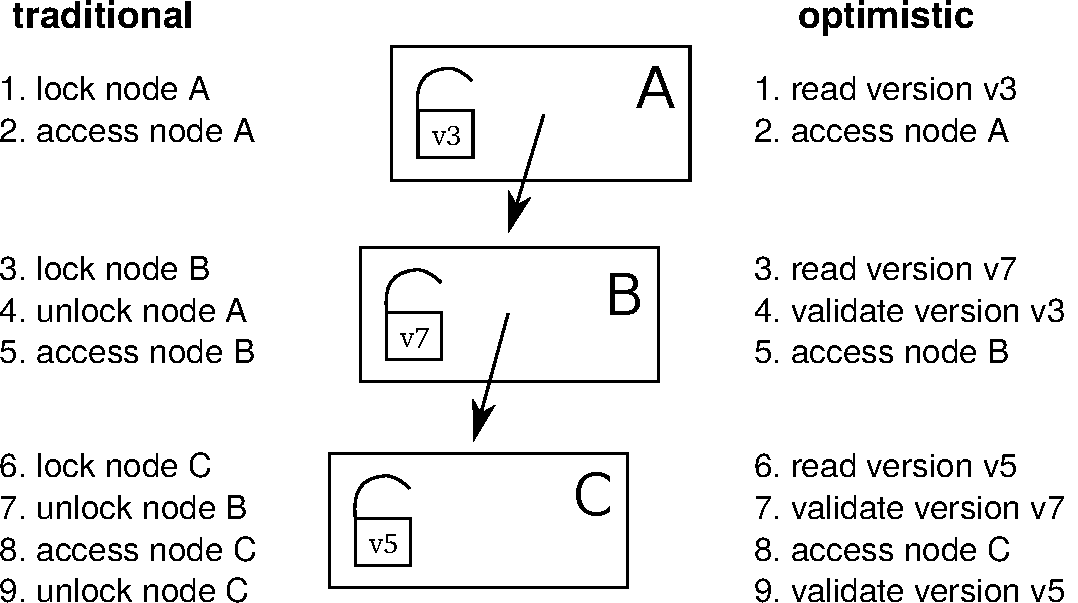
\includegraphics[width=0.65\linewidth]{olcall.pdf}
  \vspace{0.2cm}
  \caption{Comparison of a lookup operation in a 3-level tree using traditional lock coupling (left-hand side) vs.~optimistic lock coupling (right-hand side).}
  \label{fig:olc}
\end{figure}

The traditional and most common lock-based synchronization protocol for B-trees is lock coupling, which interleaves lock acquisitions while holding at most two locks at a time.
If, as we observed earlier, optimistic locks have similar semantics as traditional locks, it is natural to ask whether lock coupling can be combined with optimistic locks.
And indeed the answer is yes: One can almost mechanically translate traditional lock coupling code to optimistic lock coupling code.
This is illustrated in Figure~\ref{fig:olc}, which compares the traversal in a tree of height 3 using traditional and optimistic locks.
As the figure shows, the main difference is that locking is translated to reading the version and that unlocking becomes validation of the previously read version.
This simple change provides efficient lock-free tree traversal without the need to design a complex synchronization protocol.

It is important to emphasize the conceptual simplicity of OLC in comparison to data structures that use custom protocols like the Bw-tree~\cite{DBLP:conf/icde/LevandoskiLS13a}.
To implement lock-free access, the Bw-tree requires an indirection table, delta nodes, complex splitting and merging logic, retry logic, etc.
OLC, on the other hand, can directly be applied to B-trees mostly by adding the appropriate optimistic locking code and without modifying the node layout itself.
Therefore, OpenBw-Tree, an open source implementation of the Bw-tree, requires an order of magnitude more code than a B-tree based on OLC\footnote{Both implementations are available on GitHub: \url{https://github.com/wangziqi2016/index-microbench}}.
Given how difficult it is to develop, validate, and debug lock-free code, simplicity is obviously a major advantage.

\subsection{Correctness Aspects}

\begin{figure}
  % \centering
  %[basicstyle=\normalsize\ttfamily,showstringspaces=false,columns=fullflexible,breaklines=false,breakatwhitespace=true,numbers=none,numberstyle=\small,style=C,keepspaces=true]
\begin{lstlisting}[basicstyle=\ttfamily,language=C++,numbers=left,numberstyle=\small]
std::atomic<BTreeNode*> root;

// search for key in B+tree, returns payload in resultOut
bool lookup(Key key, Value& resultOut) {
   BTreeNode* node = root.load();
   uint64_t nodeVersion = node->readLockOrRestart();
   if (node != root.load()) // make sure the root is still the root
      restart();

   BTreeInner<Key>* parent = nullptr;
   uint64_t parentVersion = 0;

   while (node->isInner()) {
      auto inner = (BTreeInner*)node;

      // unlock parent and make current node the parent
      if (parent)
         parent->readUnlockOrRestart(parentVersion);
      parent = inner;
      parentVersion = nodeVersion;

      // search for next node
      node = inner->findChild(key);
      // validate 'inner' to ensure that 'node' pointer is valid
      inner->checkOrRestart(nodeVersion);
      // now it safe to dereference 'node' pointer (read its version)
      nodeVersion = node->readLockOrRestart();
   }

   // search in leaf and retrieve payload
   auto leaf = (BTreeLeaf*)node;
   bool success = leaf->findValue(key, resultOut);

   // unlock everything
   if (parent)
      parent->readUnlockOrRestart(parentVersion);
   node->readUnlockOrRestart(nodeVersion);

   return success;
}
\end{lstlisting}
  \vspace{0.2cm}
  \caption{B-tree lookup code using OLC. For simplicity, the restart logic is not shown.}
  \label{fig:lookup}
\end{figure}

So far, we have introduced the high-level ideas behind OLC and have stressed its similarity to traditional lock coupling.
Let us now discuss some cases where the close similarity between lock coupling and OLC breaks down.
To make this more concrete, we show the B-tree lookup code in Figure~\ref{fig:lookup}.
In the code, \texttt{readLockOrRestart} reads the lock version and \texttt{readUnlockOrRestart} validates that the read was correct.

One issue with OLC is that any pointer speculatively read from a node may point to invalid memory (if that node is modified concurrently).
Dereferencing such a pointer (e.g., to read its optimistic lock), may cause a segmentation fault or undefined behavior.
In the code shown in Figure~\ref{fig:lookup}, this problem is prevented by the extra check in line 25, which ensures that the read from the node containing the pointer was correct.
Without this additional validation, the code would in line 27 dereference the pointer speculatively read in line 23.
Note that the implementation of \texttt{checkOrRestart} is actually identical to \texttt{readUnlockOrRestart}.
We chose to give it a different name to highlight the fact that this extra check would not be necessary with read/write locks.

Another potential issue with optimistic locks is code that does not terminate.
Code that speculatively accesses a node, like an intra-node binary search, should be written in a way such that it always terminates---even in the presence of concurrent writes.
Otherwise, the validation code that detects the concurrent write will never run.
The binary search of a B-tree, for example, needs to be written in such a way that each comparison makes progress.
For some data structures that do not require loops in the traversal code (like ART) termination is trivially true.

\subsection{Implementation Details}

% implementation, efficiency
To implement an optimistic lock, one can combine the lock and the version counter into a single 64-bit\footnote{Even after subtracting one bit for the lock status, a back-of-the-envelope calculation can show that 63 bits are large enough to never overflow in practice.} word~\cite{artsync}.
A typical read operation will therefore merely consist of reading this version counter atomically.
In C++11 this can be implemented using the \texttt{std::atomic} type.

On x86, atomic reads are cheap because of x86's strong memory order guarantees.
No memory fences are required for sequentially-consistent loads, which are translated (by both GCC and clang) into standard \texttt{MOV} instructions.
Hence, the only effect of \texttt{std::atomic} for loads is preventing instruction re-ordering.
This makes version access and validation cheap.
Acquiring and releasing an optimistic lock in exclusive mode has comparable cost to a traditional lock:
A fairly expensive sequentially-consistent store is needed for acquiring a lock, while a standard \texttt{MOV} suffices for releasing it.
A simple sinlock-based implementation of optimistic locks can be found in the appendix of an earlier paper~\cite{artsync}.

OLC code must be able to handle restarts since validation or lock upgrade can fail due to concurrent writers.
Restarts can easily be implemented by wrapping the data structure operation in a loop (for simplicity not shown in Figure~\ref{fig:lookup}).
Such a loop also enables limiting the number of optimistic retry operations and falling back to pessimistic locking in cases of very heavy contention.
The ability to fall back to traditional locking is a major advantage of OLC in terms of robustness over lock-free approaches, which do not have this option.

In addition to the optimistic shared mode and the exclusive mode, optimistic locks also support a ``shared pessimistic'' mode, which physically acquires the lock in shared mode (allowing multiple concurrent readers but no writers).
This mode is useful for table (or range) scans that touch many tuples on a leaf page (which would otherwise easily abort).
Finally, let us mention that large range scans and table scans, should be broken up into several per-node traversals as is done in the LeanStore~\cite{leanstore} system.

Like all lock-free data structures, but unlike traditional locking and Hardware Transactional Memory~\cite{DBLP:conf/hpca/KarnagelDRLLSL14,DBLP:journals/pvldb/MakreshanskiLS15,htmtkde}, OLC requires care when deleting (and reusing) nodes.
The reason is that a deleting thread can never be sure that a node can be reclaimed because other threads might still be optimistically reading from that node.
Therefore, standard solutions like epoch-based reclamation~\cite{DBLP:conf/sosp/TuZKLM13}, hazard pointers~\cite{DBLP:journals/tpds/Michael04}, or optimized hazard pointers~\cite{DBLP:conf/spaa/BalmauGHZ16} need to be used.
These memory reclamation techniques are, however, largely orthogonal to the synchronization protocol itself.

%-lock-free is not a strong guarantee

\newpage
\section{Evaluation}\label{sec:evaluation}

Let us now experimentally evaluate the overhead and scalability of OLC.
For the experiments, we use an in-memory B+tree implemented in C++11 using templates, which is configured to use nodes of 4096 bytes, random 8 byte keys, and 8 byte payloads.
Based on this B-tree, we compare the following synchronization approaches:
\begin{itemize}
\item an OLC implementation\footnote{An almost identical OLC implementation is available on github: \url{https://github.com/wangziqi2016/index-microbench/tree/master/BTreeOLC}}
\item a variant based on traditional lock coupling and read/write locks
\item the unsynchronized B-tree, which obviously is only correct for read-only workloads but allows measuring the overhead of synchronization
\end{itemize}
Note that earlier work has compared the OLC implementation with a Bw-tree implementation~\cite{buzzword} and other state-of-the-art in-memory index structures.

We use a Haswell EP system with an Intel Xeon E5-2687W v3 CPU, which has 10 cores (20 ``Hyper-Threads'') and 25~MB of L3 cache.
The system is running Ubuntu 18.10 and we use GCC 8.2.0 to compile our code.
The CPU counters are obtained using the Linux perf API\footnote{We use the following convenience wrapper: \url{https://github.com/viktorleis/perfevent}}.

\begin{table}
  \caption{Performance and CPU counters for lookup and insert operations in a B-tree with 100M keys. We perform 100M operations and normalize the CPU counters by that number.}
  \label{tab:overhead}
  \centering
  \begin{tabular}{lrrrrrrr}\toprule
                    &         &        &        & instruc-  & L1     & L3     & branch \\
                    & threads & M op/s & cycles & tions & misses & misses & misses \\\midrule
lookup (no sync.)   & 1       & 1.72   & 2028   & 283     & 39.1   & 14.9   & 16.1   \\
lookup (OLC)        & 1       & 1.65   & 2107   & 370     & 43.9   & 15.1   & 16.7   \\
lookup (lock coup.) & 1       & 1.72   & 2078   & 365     & 42.3   & 16.9   & 15.7   \\\midrule
insert (no sync.)   & 1       & 1.51   & 2286   & 530     & 59.8   & 31.1   & 17.3   \\
insert (OLC)        & 1       & 1.50   & 2303   & 629     & 61.2   & 31.1   & 16.5   \\
insert (lock coup.) & 1       & 1.41   & 2473   & 644     & 61.0   & 31.0   & 17.2   \\\midrule
lookup (no sync.)   & 10      & 15.48  & 2058   & 283     & 38.6   & 15.5   & 16.0   \\
lookup (OLC)        & 10      & 14.60  & 2187   & 370     & 43.8   & 15.8   & 16.8   \\
lookup (lock coup.) & 10      & 5.71   & 5591   & 379     & 54.2   & 17.0   & 14.8   \\\midrule
insert (no sync.)   & 10      & -      & -      & -       & -      & -      & -      \\
insert (OLC)        & 10      & 10.46  & 2940   & 656     & 62.0   & 32.5   & 16.8   \\
insert (lock coup.) & 10      & 7.55   & 4161   & 667     & 75.0   & 28.6   & 16.2   \\
    \bottomrule
\end{tabular}
\end{table}

Table~\ref{tab:overhead} compares the performance and CPU counters for lookup and insert operations in a B-tree with 100M keys.
With {\em single-threaded} execution, we observe that all three approaches have very similar performance.
Adding traditional or optimistic locks to unsynchronized B-tree code results in up to 30\% of additional instructions without affecting single-threaded performance much.

\begin{figure}
  \centering
  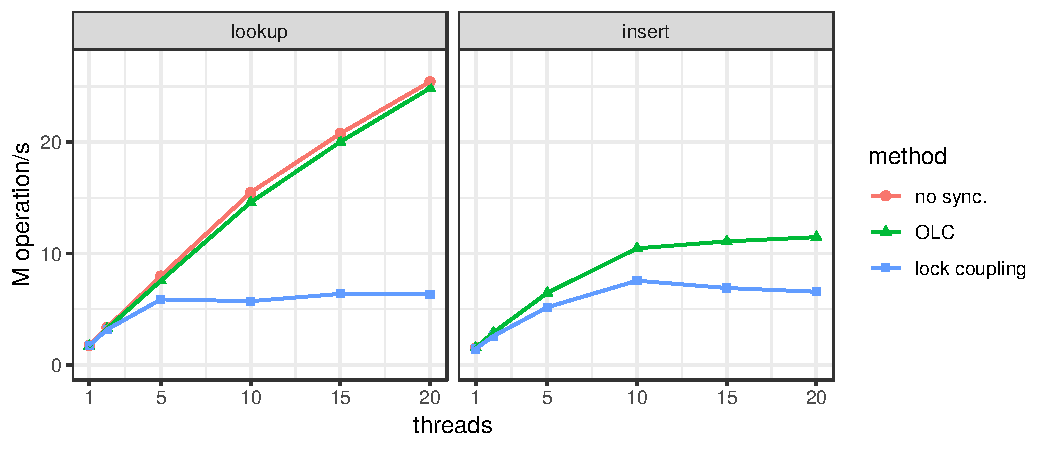
\includegraphics[width=\linewidth]{scale.pdf}
  \vspace{0.2cm}
  \caption{Scalability on 10-core system for B-tree operations (100M values).}
  \label{fig:scale}
\end{figure}

As Figure~\ref{fig:scale} shows, the results change dramatically once we use multiple threads.
For lookup, the scalability of OLC is near-linear up to 20 threads, even though the system has only 10 ``real cores''.
The OLC scalability for insert is also respectable (though not quite as linear because multi-threaded insertion approaches the memory bandwidth of our processor).
The figure also shows that the results of traditional lock coupling with read/write locks are significantly worse than OLC.
With 20 threads, lookup with OLC is 3.9$\times$ faster than traditional lock coupling.

\section{Summary}\label{sec:conc}

Optimistic Lock Coupling (OLC) is an effective synchronization method that combines the simplicity of traditional lock coupling with the superior scalability of lock-free approaches.
OLC is widely applicable and has already been successfully used to synchronize several data structures, including B-trees, binary search trees, and different trie variants.
These features make it highly attractive for modern database systems as well as performance-critical systems software in general.

\begin{thebibliography}{10}

\bibitem{DBLP:conf/spaa/BalmauGHZ16}
O.~Balmau, R.~Guerraoui, M.~Herlihy, and I.~Zablotchi.
\newblock Fast and robust memory reclamation for concurrent data structures.
\newblock In {\em SPAA}, 2016.

\bibitem{DBLP:journals/acta/BayerS77}
R.~Bayer and M.~Schkolnick.
\newblock Concurrency of operations on {B}-trees.
\newblock {\em Acta Informatica}, 9, 1977.

\bibitem{hot}
R.~Binna, E.~Zangerle, M.~Pichl, G.~Specht, and V.~Leis.
\newblock {HOT}: A height optimized trie index for main-memory database
  systems.
\newblock In {\em SIGMOD}, 2018.

\bibitem{DBLP:conf/ppopp/BronsonCCO10}
N.~G. Bronson, J.~Casper, H.~Chafi, and K.~Olukotun.
\newblock A practical concurrent binary search tree.
\newblock In {\em PPOPP}, 2010.

\bibitem{DBLP:conf/vldb/ChaHKK01}
S.~K. Cha, S.~Hwang, K.~Kim, and K.~Kwon.
\newblock Cache-conscious concurrency control of main-memory indexes on
  shared-memory multiprocessor systems.
\newblock In {\em VLDB}, 2001.

\bibitem{intel}
I.~Cutress.
\newblock {Intel} goes for 48-cores: {Cascade-AP} with multi-chip package
  coming soon.
\newblock
  \url{https://www.anandtech.com/show/13535/intel-goes-for-48cores-cascade-ap},
  2018 (accessed January, 2019).

\bibitem{DBLP:conf/cidr/FaleiroA17}
J.~M. Faleiro and D.~J. Abadi.
\newblock Latch-free synchronization in database systems: Silver bullet or
  fool's gold?
\newblock In {\em CIDR}, 2017.

\bibitem{DBLP:journals/ftdb/Graefe11}
G.~Graefe.
\newblock Modern {B}-tree techniques.
\newblock {\em Foundations and Trends in Databases}, 3(4), 2011.

\bibitem{DBLP:conf/hpca/KarnagelDRLLSL14}
T.~Karnagel, R.~Dementiev, R.~Rajwar, K.~Lai, T.~Legler, B.~Schlegel, and
  W.~Lehner.
\newblock Improving in-memory database index performance with
  {Intel}\({}^{\mbox{{\textregistered}}}\) transactional synchronization
  extensions.
\newblock In {\em HPCA}, 2014.

\bibitem{DBLP:journals/tods/LehmanY81}
P.~L. Lehman and S.~B. Yao.
\newblock Efficient locking for concurrent operations on {B}-trees.
\newblock {\em {ACM} Trans. Database Syst.}, 6(4), 1981.

\bibitem{leanstore}
V.~Leis, M.~Haubenschild, A.~Kemper, and T.~Neumann.
\newblock Leanstore: In-memory data management beyond main memory.
\newblock In {\em ICDE}, 2018.

\bibitem{art}
V.~Leis, A.~Kemper, and T.~Neumann.
\newblock The adaptive radix tree: {ARTful} indexing for main-memory databases.
\newblock In {\em ICDE}, 2013.

\bibitem{htmtkde}
V.~Leis, A.~Kemper, and T.~Neumann.
\newblock Scaling {HTM}-supported database transactions to many cores.
\newblock {\em {IEEE} Trans. Knowl. Data Eng.}, 28(2), 2016.

\bibitem{artsync}
V.~Leis, F.~Scheibner, A.~Kemper, and T.~Neumann.
\newblock The {ART} of practical synchronization.
\newblock In {\em DaMoN}, 2016.

\bibitem{DBLP:conf/icde/LevandoskiLS13a}
J.~J. Levandoski, D.~B. Lomet, and S.~Sengupta.
\newblock The {Bw}-tree: A {B}-tree for new hardware platforms.
\newblock In {\em ICDE}, 2013.

\bibitem{DBLP:journals/pvldb/MakreshanskiLS15}
D.~Makreshanski, J.~J. Levandoski, and R.~Stutsman.
\newblock To lock, swap, or elide: On the interplay of hardware transactional
  memory and lock-free indexing.
\newblock {\em {PVLDB}}, 8(11), 2015.

\bibitem{DBLP:dblp_conf/eurosys/MaoKM12}
Y.~Mao, E.~Kohler, and R.~T. Morris.
\newblock Cache craftiness for fast multicore key-value storage.
\newblock In {\em EuroSys}, 2012.

\bibitem{DBLP:journals/tpds/Michael04}
M.~M. Michael.
\newblock Hazard pointers: Safe memory reclamation for lock-free objects.
\newblock {\em {IEEE} Trans. Parallel Distrib. Syst.}, 15(6), 2004.

\bibitem{DBLP:journals/jacm/ShalevS06}
O.~Shalev and N.~Shavit.
\newblock Split-ordered lists: Lock-free extensible hash tables.
\newblock {\em J. {ACM}}, 53(3), 2006.

\bibitem{amd}
A.~Shilov.
\newblock {AMD} previews {EPYC} ‘{Rome}’ processor: Up to 64 {Zen} 2 cores.
\newblock
  \url{https://www.anandtech.com/show/13561/amd-previews-epyc-rome-processor-up-to-64-zen-2-cores},
  2018 (accessed January, 2019).

\bibitem{DBLP:conf/sosp/TuZKLM13}
S.~Tu, W.~Zheng, E.~Kohler, B.~Liskov, and S.~Madden.
\newblock Speedy transactions in multicore in-memory databases.
\newblock In {\em SOSP}, 2013.

\bibitem{buzzword}
Z.~Wang, A.~Pavlo, H.~Lim, V.~Leis, H.~Zhang, M.~Kaminsky, and D.~Andersen.
\newblock Building a {Bw}-tree takes more than just buzz words.
\newblock In {\em SIGMOD}, 2018.

\end{thebibliography}


%\bibliographystyle{abbrv}
%\bibliography{main}

\end{document}

\end{article}








\end{articlesection}

% put the news items below- there can be multiple news sections
% each with its own title
% news will usually have an author as well as a title, 
% e.g. TCDE elections
% news articles are in the same format as letters
% typically, news articles will be stored in a directory called "news"

%\begin{newssection}{News headline}

% insert news items here; news will typically have authors
% see the Sept. 2018 issue for an example

%\begin{news}{news item title}
%{author name}{author affiliation}
%\input{news/news-article.tex}
%\end{news}
%
%\newpage


%\end{newssection}

\begin{callsection}

%  This section will be empty for your version
%
%  Calls for papers section.  Use the callsection environment.
%  Each call for papers is contained in an call environment, where the single 
%  required options to \begin{call} is the name of the conference.
% typically calls are stored in a "calls" directory
%
%\begin{call}{name of conference}
%\centerline{\includegraphics[width=\textwidth, bb= 0 0 590 760]{calls/conference-name.pdf}}
%\end{call}
%\begin{call}{ICDE 2019 Conference}
%\centerline{
\includegraphics[width=\textwidth, bb= 0 0 610 790] {../Dec-2018/calls/icde19.pdf}} 
%\centerline{
\includegraphics[width=\textwidth, bb= 0 0 590 760] {calls/icde19.pdf}}
%\end{call}
\begin{call}{TCDE Membership Form}
%\centerline{\includegraphics[width=\textwidth, bb= 0 0 610 790]
%\centerline{
\includegraphics[width=\textwidth, bb= 0 0 590 760] {../Dec-2018/calls/tcde.pdf}}
\centerline{
\includegraphics[width=\textwidth, bb= 0 0 590 760] {../2020-09/calls/tcde.pdf}}
\end{call}

\end{callsection}

\end{bulletin}
\end{document}
